\section{Resultados}\label{sec:resultados}

\subsection{Valida\c{c}\~{a}o do Modelo BP SB-FET e Caracteriza\c{c}\~{a}o do Dispositivo}\label{sec:res_modelo}

A biblioteca comportamental nativa \texttt{bp\_ari\_ngspice.lib} (\texttt{v2}) reproduziu as superf\'{i}cies experimentais de transfer\^{e}ncia e sa\'{i}da em todo o plano operacional medido. A Tabela~\ref{tab:metricas_dispositivo} consolida os par\^{a}metros el\'{e}tricos extra\'{i}dos em $|V_{ds}| = 0{,}8\ \text{V}$, evidenciando erro m\'{e}dio relativo frente \`{a}s tabelas LUT de apenas $0{,}0621\%$ no modo \textit{n-FET} e $0{,}0032\%$ no modo \textit{p-FET}. Ressalta-se que os valores de inclina\c{c}\~{a}o de sublimiar ($106{,}59\text{--}148{,}08\ \text{mV/dec}$) e raz\~{a}o $I_{\mathrm{on}}/I_{\mathrm{off}}$ obtidos refletem estritamente a condi\c{c}\~{a}o de $|V_{ds}| = 0{,}8\ \text{V}$ na qual as tabelas compactas \texttt{BP\_ARI\_dataN/P.txt} foram registradas, diferenciando-se das condi\c{c}\~{o}es de baixa polariza\c{c}\~{a}o de dreno ($|V_{ds}| = 0{,}1\ \text{V}$, $SS = 72\text{--}75\ \text{mV/dec}$) e maior \textit{overdrive} reportadas em~\cite{wu2020reconfigurable}.

\begin{table}[htbp]
\centering
\caption{M\'{e}tricas el\'{e}tricas do dispositivo BP SB-FET extra\'{i}das no \texttt{ngspice-47} ($|V_{ds}|=0{,}8\ \text{V}$).}
\label{tab:metricas_dispositivo}
\resizebox{\textwidth}{!}{%
\begin{tabular}{l c c c c c}
\toprule
\textbf{Modo e Polariza\c{c}\~{a}o} & $I_{\mathrm{on}}$ ($\mu\text{A}/\mu\text{m}$) & $I_{\mathrm{off}}$ ($\text{nA}/\mu\text{m}$) & \textbf{Raz\~{a}o} $I_{\mathrm{on}}/I_{\mathrm{off}}$ & $SS_{\min}$ ($\text{mV/dec}$) & \textbf{Erro M\'{e}dio vs.\ LUT (\%)} \\
\midrule
\textit{n-FET} ($V_{g1}=1{,}1\ \text{V},\ V_{g2}=0{,}8\ \text{V}$) & $1{,}650$ & $0{,}596$ & $2{,}77 \times 10^3$ & $106{,}59$ & $0{,}0621\%$ \\
\textit{n-FET} ($V_{g1}=0{,}9\ \text{V},\ V_{g2}=0{,}8\ \text{V}$) & $1{,}110$ & $0{,}588$ & $1{,}89 \times 10^3$ & $108{,}48$ & $0{,}0621\%$ \\
\textit{p-FET} ($V_{g1}=-1{,}5\ \text{V},\ V_{g2}=-1{,}2\ \text{V}$) & $1{,}790$ & $2{,}811$ & $6{,}37 \times 10^2$ & $148{,}08$ & $0{,}0032\%$ \\
\bottomrule
\end{tabular}}
\end{table}

Na valida\c{c}\~{a}o cruzada direta contra os arquivos de refer\^{e}ncia \texttt{.printtr0} do Synopsys HSPICE (Tabela~\ref{tab:validacao_hspice}), o refinamento 4D (\texttt{v2}) demonstrou ganhos expressivos em rela\c{c}\~{a}o \`{a} aproxima\c{c}\~{a}o preliminar \texttt{v1} (1D + $\tanh$). Nos regimes de transfer\^{e}ncia, ambos os modelos alcan\c{c}aram $R^2 \ge 0{,}99994$ ($\text{RMSE} < 0{,}002\ \mu\text{A}/\mu\text{m}$). O ganho mais expressivo ocorreu no regime \texttt{P\_output} ($V_{g2} = -1{,}5\ \text{V}$): na \texttt{v1}, a escala emp\'{i}rica sobre $V_{g2}=-1{,}2\ \text{V}$ superestimava a corrente em at\'{e} $8{,}9\times$ ($R^2 = -7{,}6723$); ao incorporar a superf\'{i}cie experimental completa de $V_{g2}=-1{,}5\ \text{V}$, a \texttt{v2} reduziu o RMSE em $99{,}5\%$ (de $0{,}590087$ para $0{,}003013\ \mu\text{A}/\mu\text{m}$, melhoria de \textbf{196$\times$}) e elevou $R^2$ para $0{,}999774$. No regime \texttt{N\_output}, o RMSE caiu $33{,}6\%$ ($0{,}196416 \to 0{,}130430\ \mu\text{A}/\mu\text{m}$, $R^2 = 0{,}927855$), sendo o desvio residual atribu\'{i}do a uma descontinuidade de lote nos pr\'{o}prios dados de \texttt{BP\_ARI\_dataN.txt} entre a varredura de transfer\^{e}ncia em $V_{ds}=0{,}80\ \text{V}$ ($I_d = 1{,}650\ \mu\text{A}$) e a varredura de sa\'{i}da adjacente em $V_{ds}=0{,}79/0{,}81\ \text{V}$ ($1{,}465\text{--}1{,}470\ \mu\text{A}$). Adicionalmente, o travamento plano de \texttt{v2} suprimiu invers\~{o}es n\~{a}o f\'{i}sicas de sinal geradas pela extrapola\c{c}\~{a}o linear \texttt{"1LL"} do HSPICE fora dos limites da tabela.

\begin{table}[htbp]
\centering
\caption{Valida\c{c}\~{a}o cruzada quantitativa entre \texttt{ngspice-47} (\texttt{v1} e \texttt{v2}) e arquivos \texttt{.printtr0} do HSPICE.}
\label{tab:validacao_hspice}
\resizebox{\textwidth}{!}{%
\begin{tabular}{l c c c c c c c}
\toprule
\textbf{Regime (HSPICE)} & $\text{RMSE}_{\mathrm{v1}}$ ($\mu\text{A}$) & $\text{RMSE}_{\mathrm{v2}}$ ($\mu\text{A}$) & \textbf{Redu\c{c}\~{a}o RMSE} & $\text{MaxErr}_{\mathrm{v1}}$ ($\mu\text{A}$) & $\text{MaxErr}_{\mathrm{v2}}$ ($\mu\text{A}$) & $R^2_{\mathrm{v1}}$ & $R^2_{\mathrm{v2}}$ \\
\midrule
\texttt{N\_transfer} (7 curvas $V_{g1}$) & $0{,}001910$ & $0{,}001899$ & $-0{,}6\%$ & $0{,}01256$ & $0{,}01256$ & $0{,}999971$ & $0{,}999972$ \\
\texttt{P\_transfer} (4 curvas $V_{g1}$) & $0{,}000947$ & $0{,}000947$ & $0{,}0\%$ & $0{,}00661$ & $0{,}00661$ & $0{,}999944$ & $0{,}999944$ \\
\texttt{N\_output} (6 curvas $V_g$) & $0{,}196416$ & $0{,}130430$ & $-33{,}6\%$ & $0{,}48360$ & $0{,}20747$ & $0{,}836392$ & $0{,}927855$ \\
\texttt{P\_output} (3 curvas $V_{g2}=-1{,}5\ \text{V}$) & $0{,}590087$ & $0{,}003013$ & $-99{,}5\%$ ($196\times$) & $0{,}90445$ & $0{,}01403$ & $-7{,}6723$ & $0{,}999774$ \\
\bottomrule
\end{tabular}}
\end{table}

As Figuras~\ref{fig:m00_transfer}, \ref{fig:m00_output}, \ref{fig:m00_pg} e \ref{fig:m00_hspice} ilustram, respectivamente, as curvas de transfer\^{e}ncia lineares e logar\'{i}tmicas (incluindo o ramo ambipolar), as fam\'{i}lias de sa\'{i}da nos dois quadrantes, a modula\c{c}\~{a}o eletrost\'{a}tica da porta de polaridade $V_{g2}$ (evidenciando a queda de banda plana em $V_{g2}=-1{,}5\ \text{V}$) e o confronto visual direto entre \texttt{v1}, \texttt{v2} e HSPICE.

\begin{figure}[htbp]
\centering
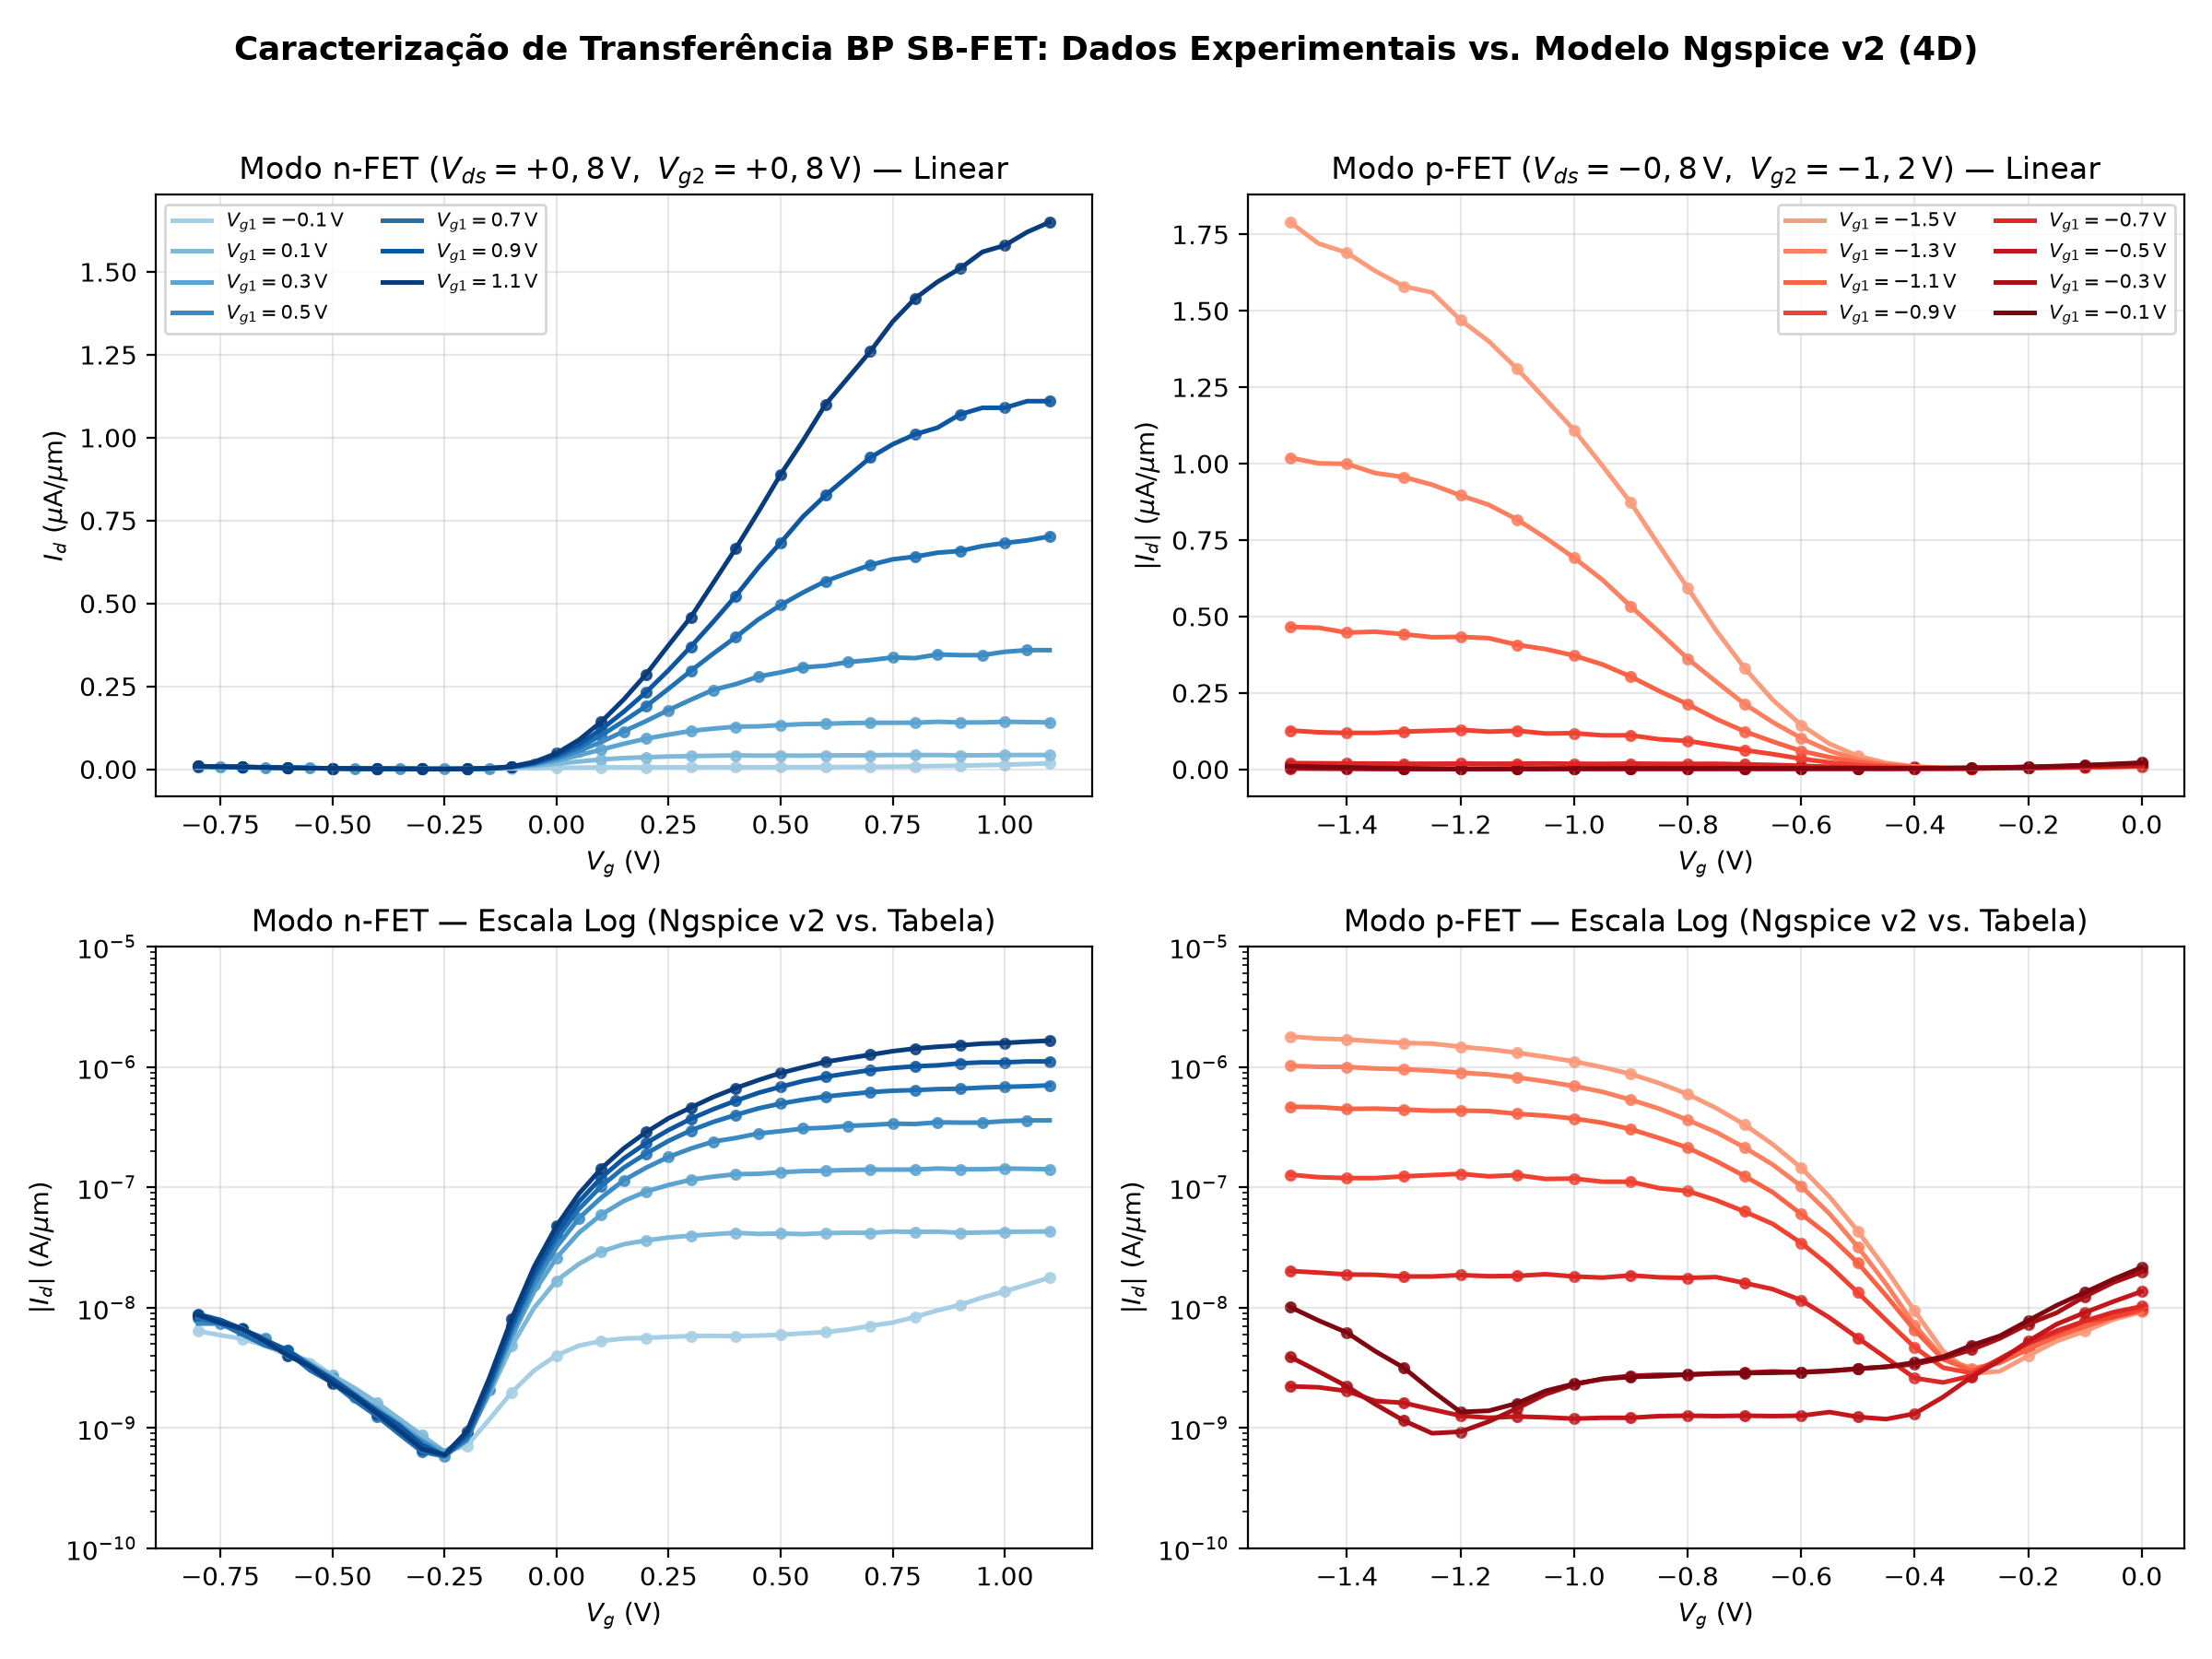
\includegraphics[width=0.92\textwidth]{m00_transfer_NP_log_lin.png}
\caption{Curvas de transfer\^{e}ncia ($I_d \times V_g$) em escalas linear e logar\'{i}tmica no \texttt{ngspice-47} comparadas aos pontos experimentais para os modos \textit{n-FET} e \textit{p-FET}.}
\label{fig:m00_transfer}
\end{figure}

\begin{figure}[htbp]
\centering
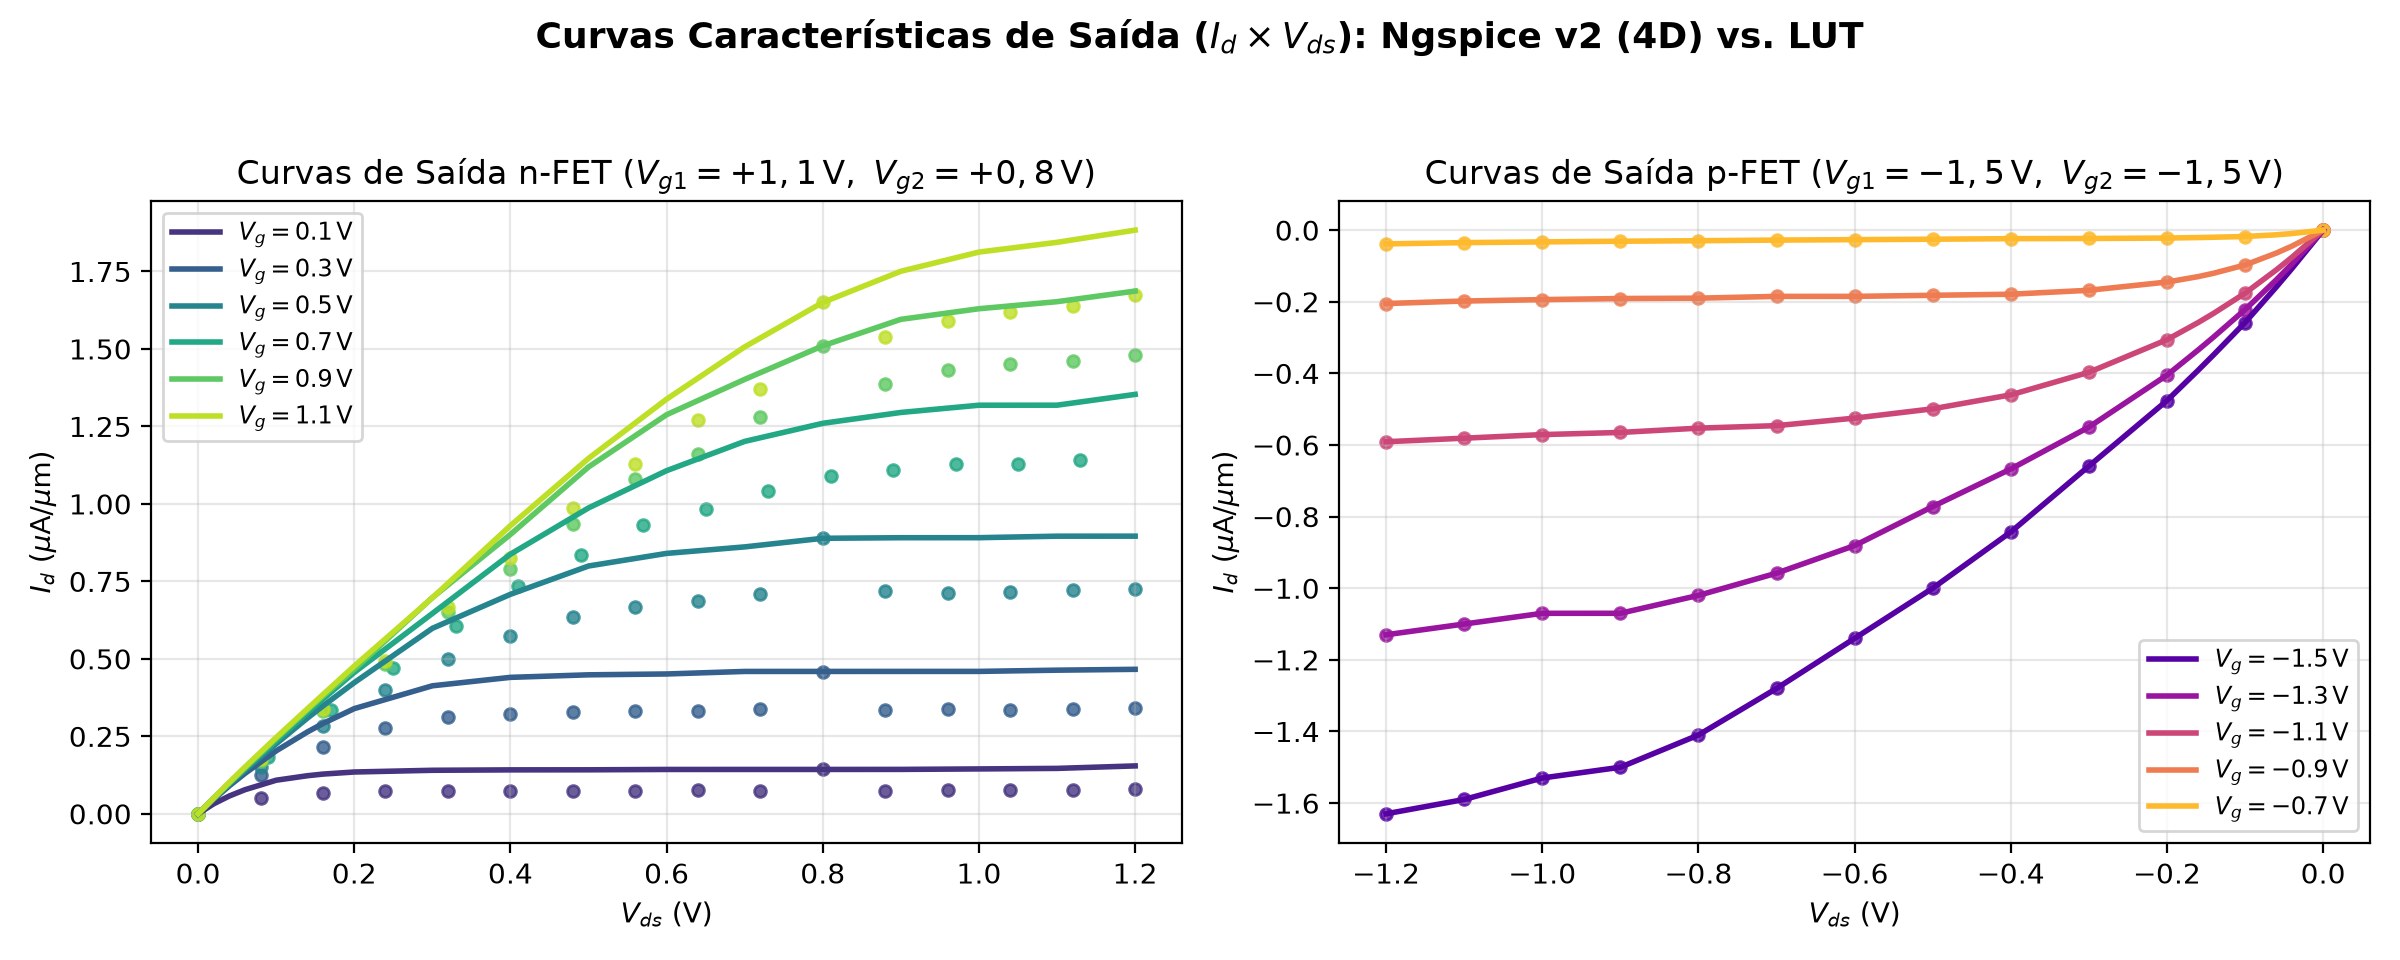
\includegraphics[width=0.92\textwidth]{m00_output_NP.png}
\caption{Fam\'{i}lias de curvas de sa\'{i}da ($I_d \times V_{ds}$) nos regimes \textit{n-FET} ($V_{ds}>0$) e \textit{p-FET} ($V_{ds}<0$, $V_{g2}=-1{,}5\ \text{V}$) reproduzindo a transi\c{c}\~{a}o tr\'{i}odo-satura\c{c}\~{a}o por porta.}
\label{fig:m00_output}
\end{figure}

\begin{figure}[htbp]
\centering
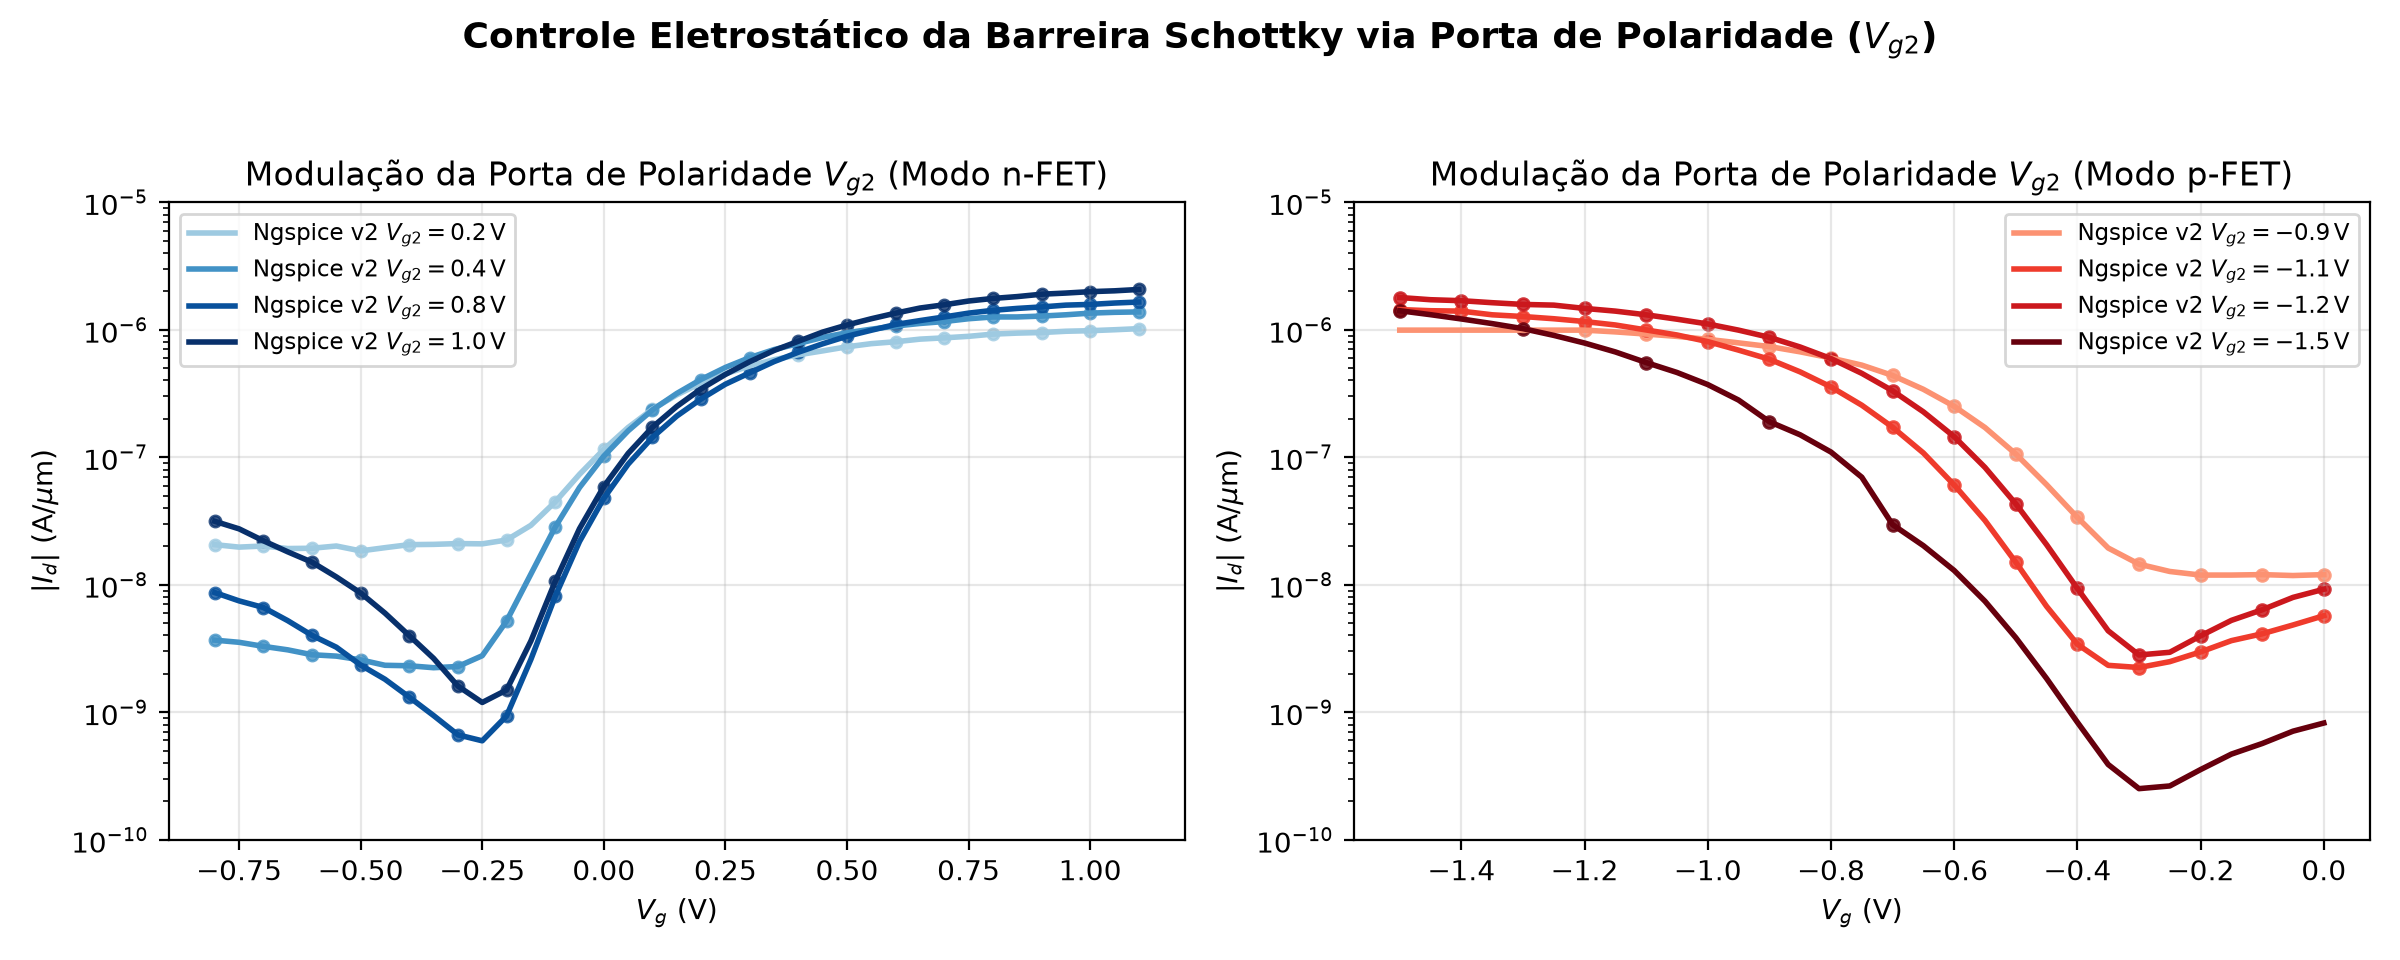
\includegraphics[width=0.92\textwidth]{m00_efeito_porta_polaridade.png}
\caption{Modula\c{c}\~{a}o eletrost\'{a}tica da porta de polaridade $V_{g2}$ sobre a corrente de canal no \textit{n-FET} e \textit{p-FET}, destacando o deslocamento de banda plana em $V_{g2}=-1{,}5\ \text{V}$.}
\label{fig:m00_pg}
\end{figure}

\begin{figure}[htbp]
\centering
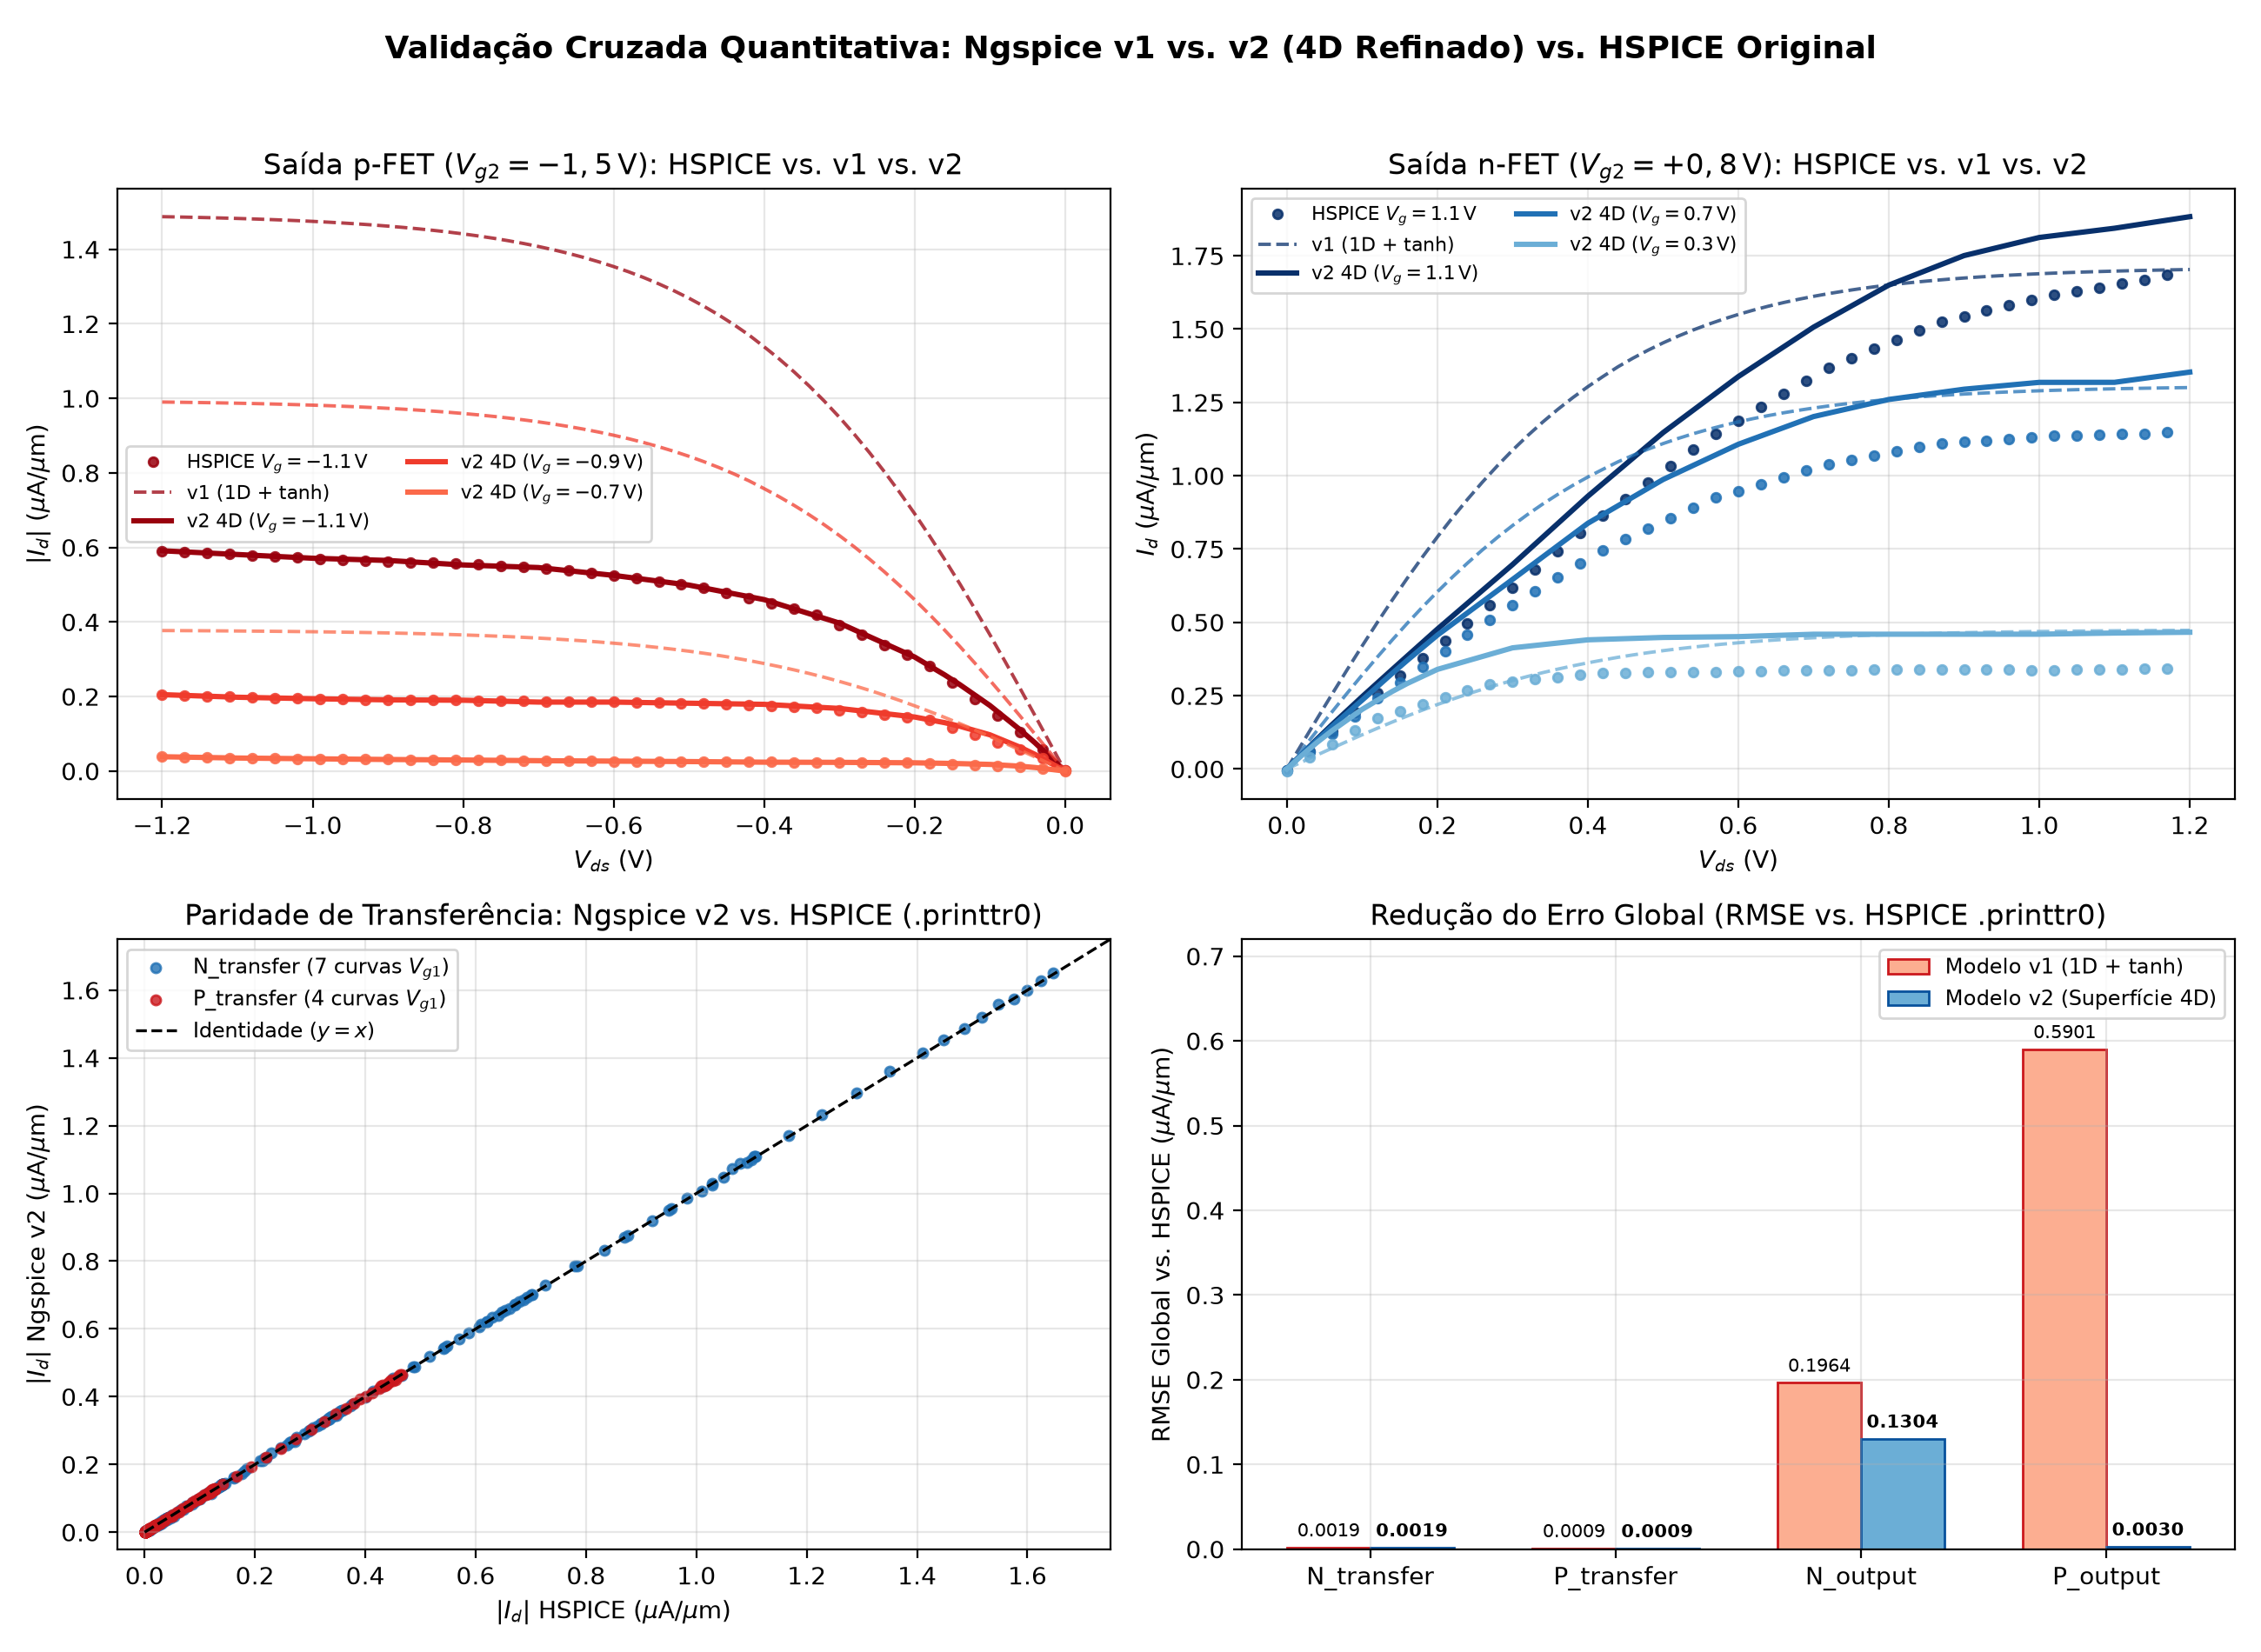
\includegraphics[width=0.92\textwidth]{m00_validacao_cruzada_hspice.png}
\caption{Valida\c{c}\~{a}o cruzada quantitativa entre o modelo preliminar (\texttt{v1}), o modelo 4D refinado (\texttt{v2}) no \texttt{ngspice-47} e as sa\'{i}das de refer\^{e}ncia \texttt{.printtr0} do Synopsys HSPICE.}
\label{fig:m00_hspice}
\end{figure}

\subsection{Inversor Complementar em Ultra-Baixa Tens\~{a}o}\label{sec:res_inversor}

Os resultados est\'{a}ticos do inversor complementar BP SB-FET entre $V_{DD} = 1{,}0\ \text{V}$ e $0{,}2\ \text{V}$ est\~{a}o compilados na Tabela~\ref{tab:inversor_vtc}. Sem compensa\c{c}\~{a}o de $V_{fb}$ (acoplamento direto), o desalinhamento entre os limiares dos ramos \textit{p-FET} e \textit{n-FET} desloca a tens\~{a}o de invers\~{a}o $V_M$ para pr\'{o}ximo de $0\ \text{V}$, colapsando completamente a fun\c{c}\~{a}o inversora em $V_{DD} \le 0{,}4\ \text{V}$ (excurs\~{a}o de $2{,}77\%$ e $|A_v|_{\max} = 0{,}37$ em $0{,}4\ \text{V}$; excurs\~{a}o de $1{,}27\%$ e ganho $0{,}06$ em $0{,}2\ \text{V}$).

\begin{table}[htbp]
\centering
\caption{M\'{e}tricas est\'{a}ticas do inversor complementar BP SB-FET sob escalonamento de $V_{DD}$ ($1{,}0\ \text{V}$ a $0{,}2\ \text{V}$).}
\label{tab:inversor_vtc}
\resizebox{\textwidth}{!}{%
\begin{tabular}{l c c c c c c c c}
\toprule
\textbf{Configura\c{c}\~{a}o} & $V_{DD}$ (V) & $V_{\mathrm{out}}(0)$ (V) & $V_{\mathrm{out}}(V_{DD})$ (V) & \textbf{Excurs\~{a}o (\%)} & $V_M$ (V) & $|A_v|_{\max}$ & $NM_L$ (V) & $NM_H$ (V) \\
\midrule
Direto (Sem comp.\ $V_{fb}$) & $1{,}0$ & $0{,}991$ & $0{,}004$ & $98{,}67\%$ & $0{,}278$ & $22{,}03$ & $0{,}096$ & $0{,}564$ \\
Direto (Sem comp.\ $V_{fb}$) & $0{,}8$ & $0{,}788$ & $0{,}004$ & $98{,}12\%$ & $0{,}162$ & $39{,}32$ & $0{,}034$ & $0{,}537$ \\
Direto (Sem comp.\ $V_{fb}$) & $0{,}6$ & $0{,}559$ & $0{,}003$ & $92{,}68\%$ & $0{,}066$ & $37{,}24$ & $0{,}000$ & $0{,}475$ \\
Direto (Sem comp.\ $V_{fb}$) & $0{,}4$ & $0{,}014$ & $0{,}003$ & $2{,}77\%$  & $0{,}010$ & $0{,}37$  & $0{,}000$ & $0{,}000$ \\
Direto (Sem comp.\ $V_{fb}$) & $0{,}2$ & $0{,}005$ & $0{,}003$ & $1{,}27\%$  & $0{,}006$ & $0{,}06$  & $0{,}000$ & $0{,}000$ \\
\midrule
Compensado ($V_{fb}$ alinhado) & $1{,}0$ & $0{,}999$ & $0{,}003$ & $99{,}63\%$ & $0{,}540$ & $54{,}69$ & $0{,}461$ & $0{,}373$ \\
Compensado ($V_{fb}$ alinhado) & $0{,}8$ & $0{,}800$ & $0{,}002$ & $99{,}75\%$ & $0{,}438$ & $50{,}84$ & $0{,}362$ & $0{,}278$ \\
Compensado ($V_{fb}$ alinhado) & $0{,}6$ & $0{,}600$ & $0{,}001$ & $99{,}80\%$ & $0{,}336$ & $38{,}18$ & $0{,}266$ & $0{,}178$ \\
Compensado ($V_{fb}$ alinhado) & $0{,}4$ & $0{,}400$ & $0{,}003$ & $99{,}29\%$ & $0{,}234$ & $12{,}71$ & $0{,}172$ & $0{,}076$ \\
Compensado ($V_{fb}$ alinhado) & $0{,}2$ & $0{,}198$ & $0{,}018$ & $89{,}75\%$ & $0{,}126$ & $2{,}71$  & $0{,}080$ & $0{,}000$ \\
\bottomrule
\end{tabular}}
\end{table}

Com o alinhamento eletrost\'{a}tico de $V_{fb}$, a tens\~{a}o de invers\~{a}o centraliza-se pr\'{o}ximo a $V_{DD}/2$ (Figura~\ref{fig:m01_vtc}), sustentando excurs\~{a}o superior a $99{,}2\%$ de $1{,}0\ \text{V}$ at\'{e} $0{,}4\ \text{V}$ e atingindo pico de ganho $|A_v|_{\max} = 54{,}69$ ($1{,}0\ \text{V}$) e $38{,}18$ ($0{,}6\ \text{V}$). Mesmo no regime extremo de ultra-baixa tens\~{a}o ($V_{DD} = 0{,}2\ \text{V}$), o inversor preserva excurs\~{a}o de $89{,}75\%$ e ganho diferencial de $2{,}71 > 1$, condição necess\'{a}ria para regenera\c{c}\~{a}o l\'{o}gica. Em regime transiente sob $C_{\mathrm{load}} = 0{,}5\ \text{fF}$ (Figura~\ref{fig:m01_tran}), as transi\c{c}\~{o}es ocorrem na escala de nanossegundos com corrente est\'{a}tica na ordem de nanoamperes e picos din\^{a}micos de $1{,}28\ \mu\text{A}$ em $1{,}0\ \text{V}$ e $0{,}73\ \mu\text{A}$ em $0{,}6\ \text{V}$.

\begin{figure}[htbp]
\centering
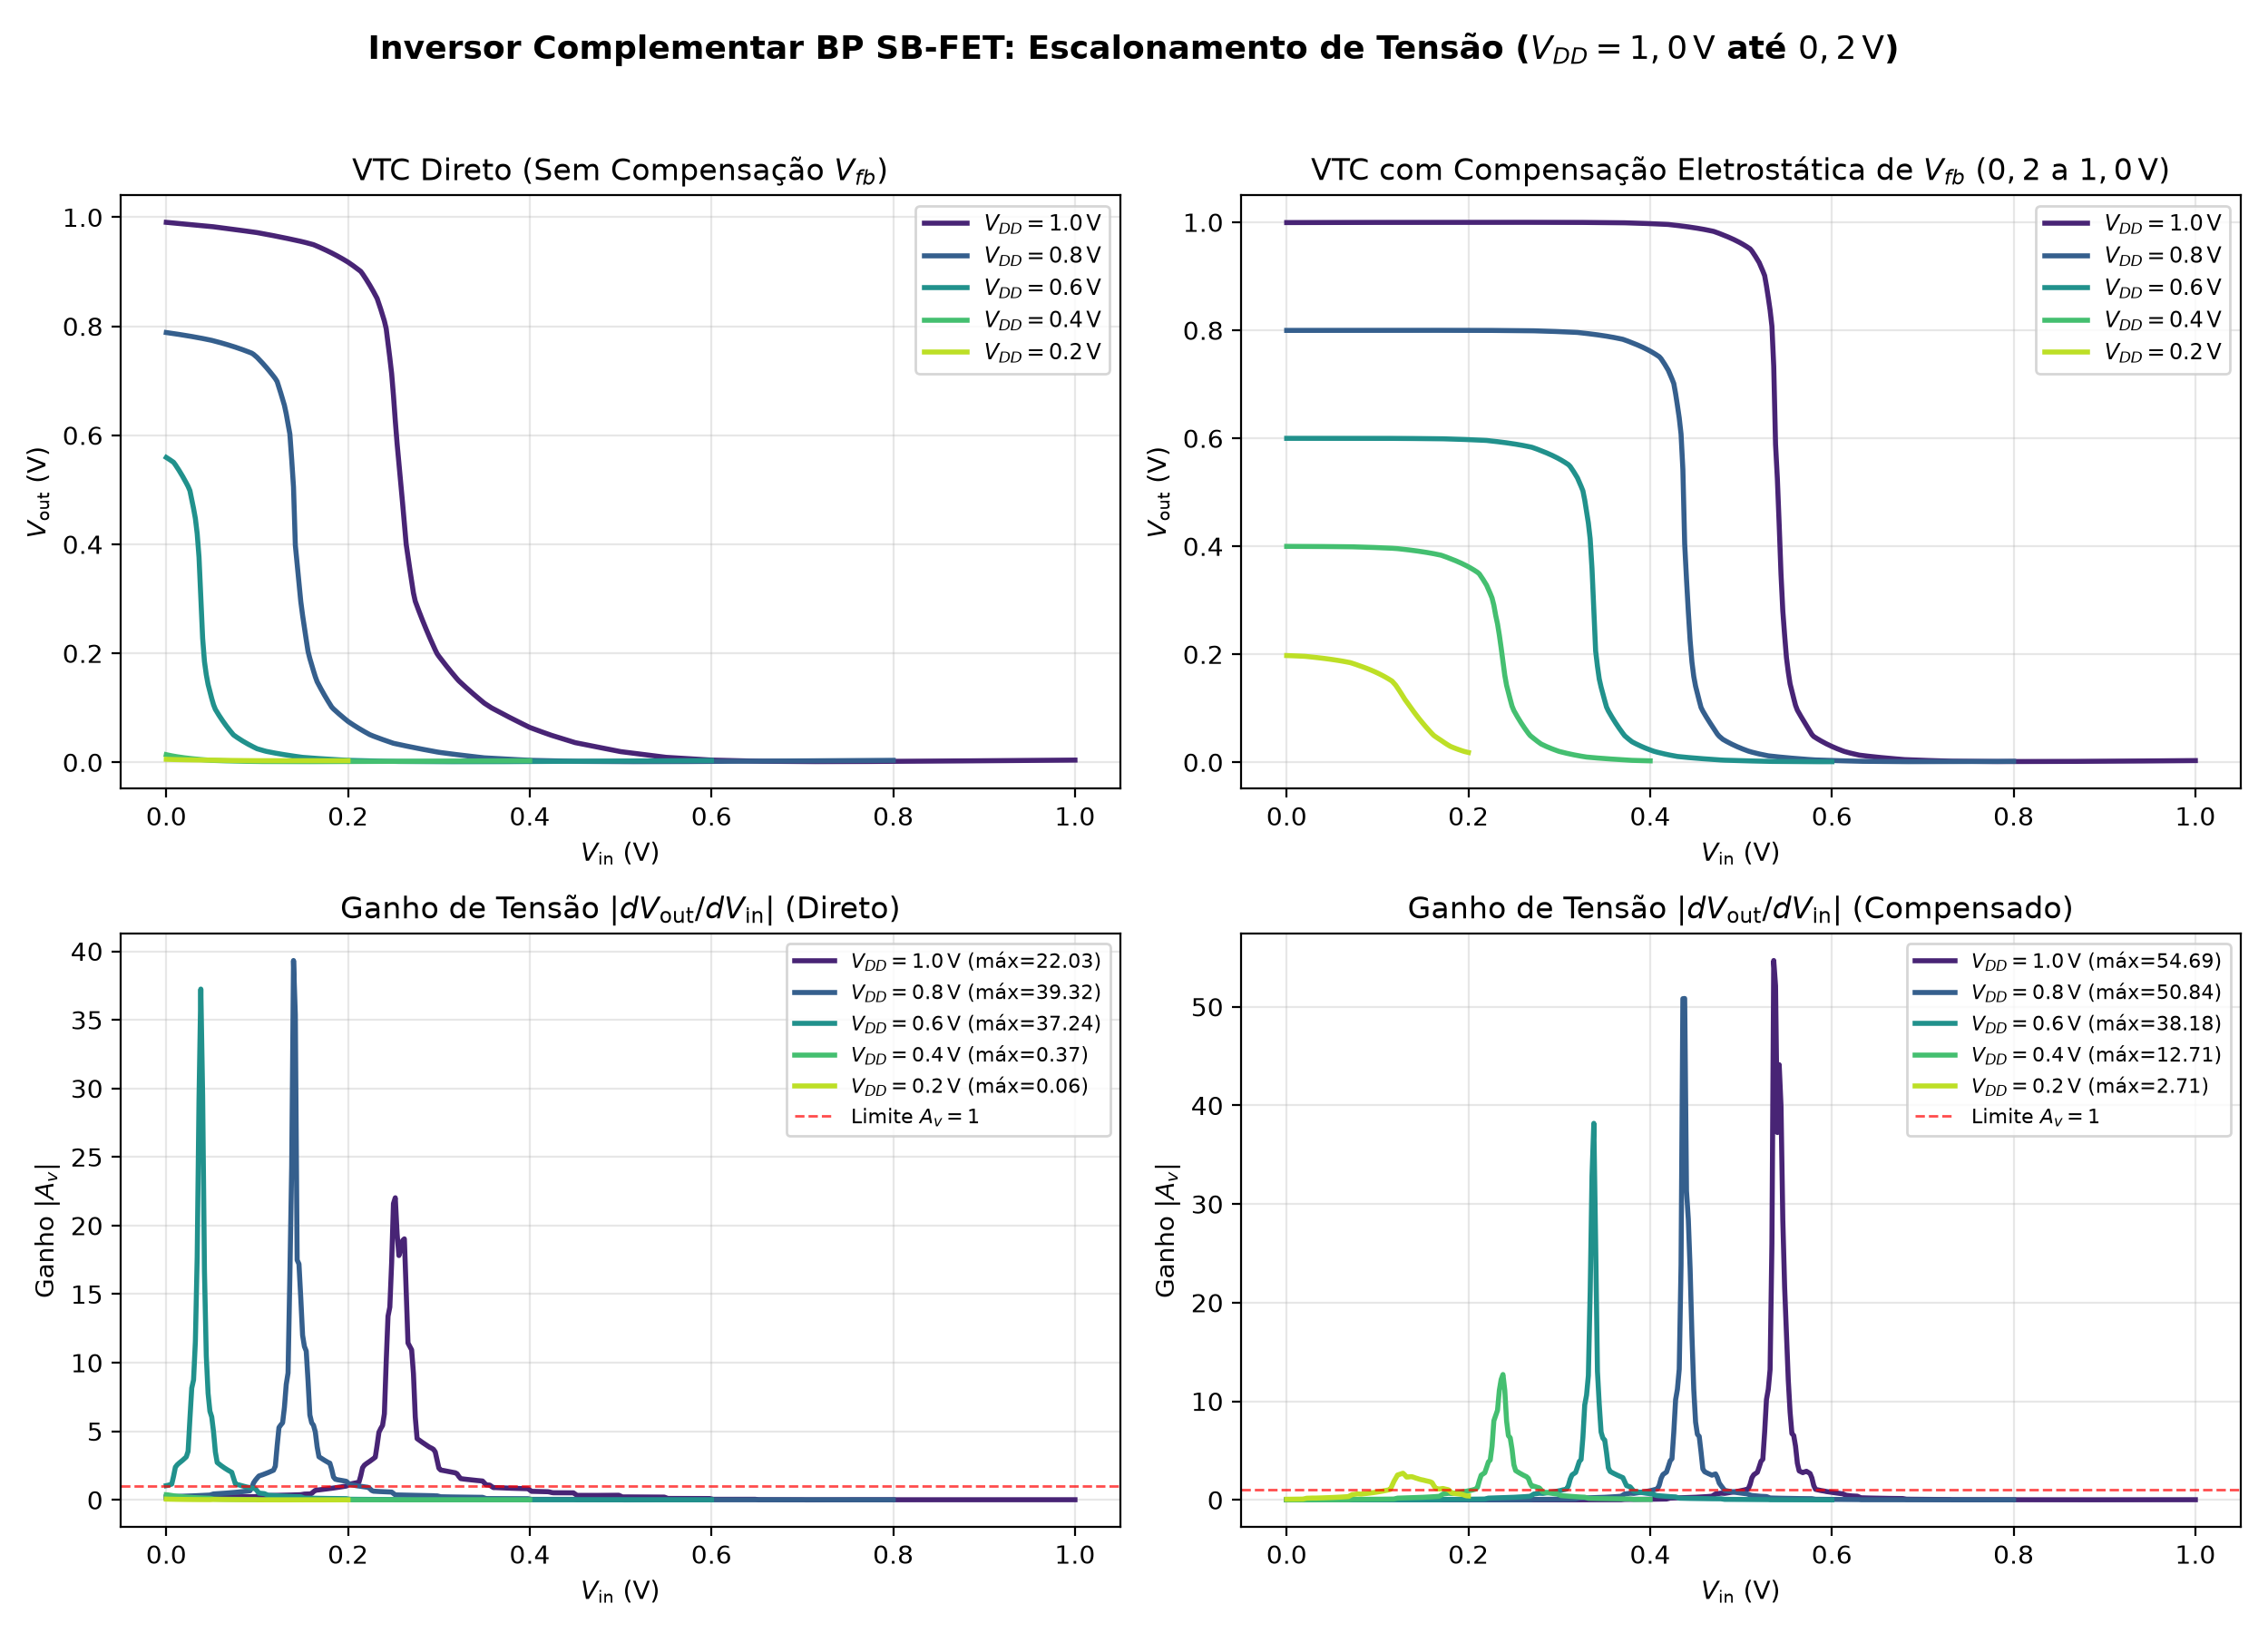
\includegraphics[width=0.92\textwidth]{m01_inversor_vtc_ganho.png}
\caption{Curvas de transfer\^{e}ncia de tens\~{a}o (VTC) e ganho diferencial $|dV_{\mathrm{out}}/dV_{\mathrm{in}}|$ do inversor BP SB-FET sem compensa\c{c}\~{a}o (esquerda) e com alinhamento de $V_{fb}$ (direita) de $1{,}0\ \text{V}$ a $0{,}2\ \text{V}$.}
\label{fig:m01_vtc}
\end{figure}

\begin{figure}[htbp]
\centering
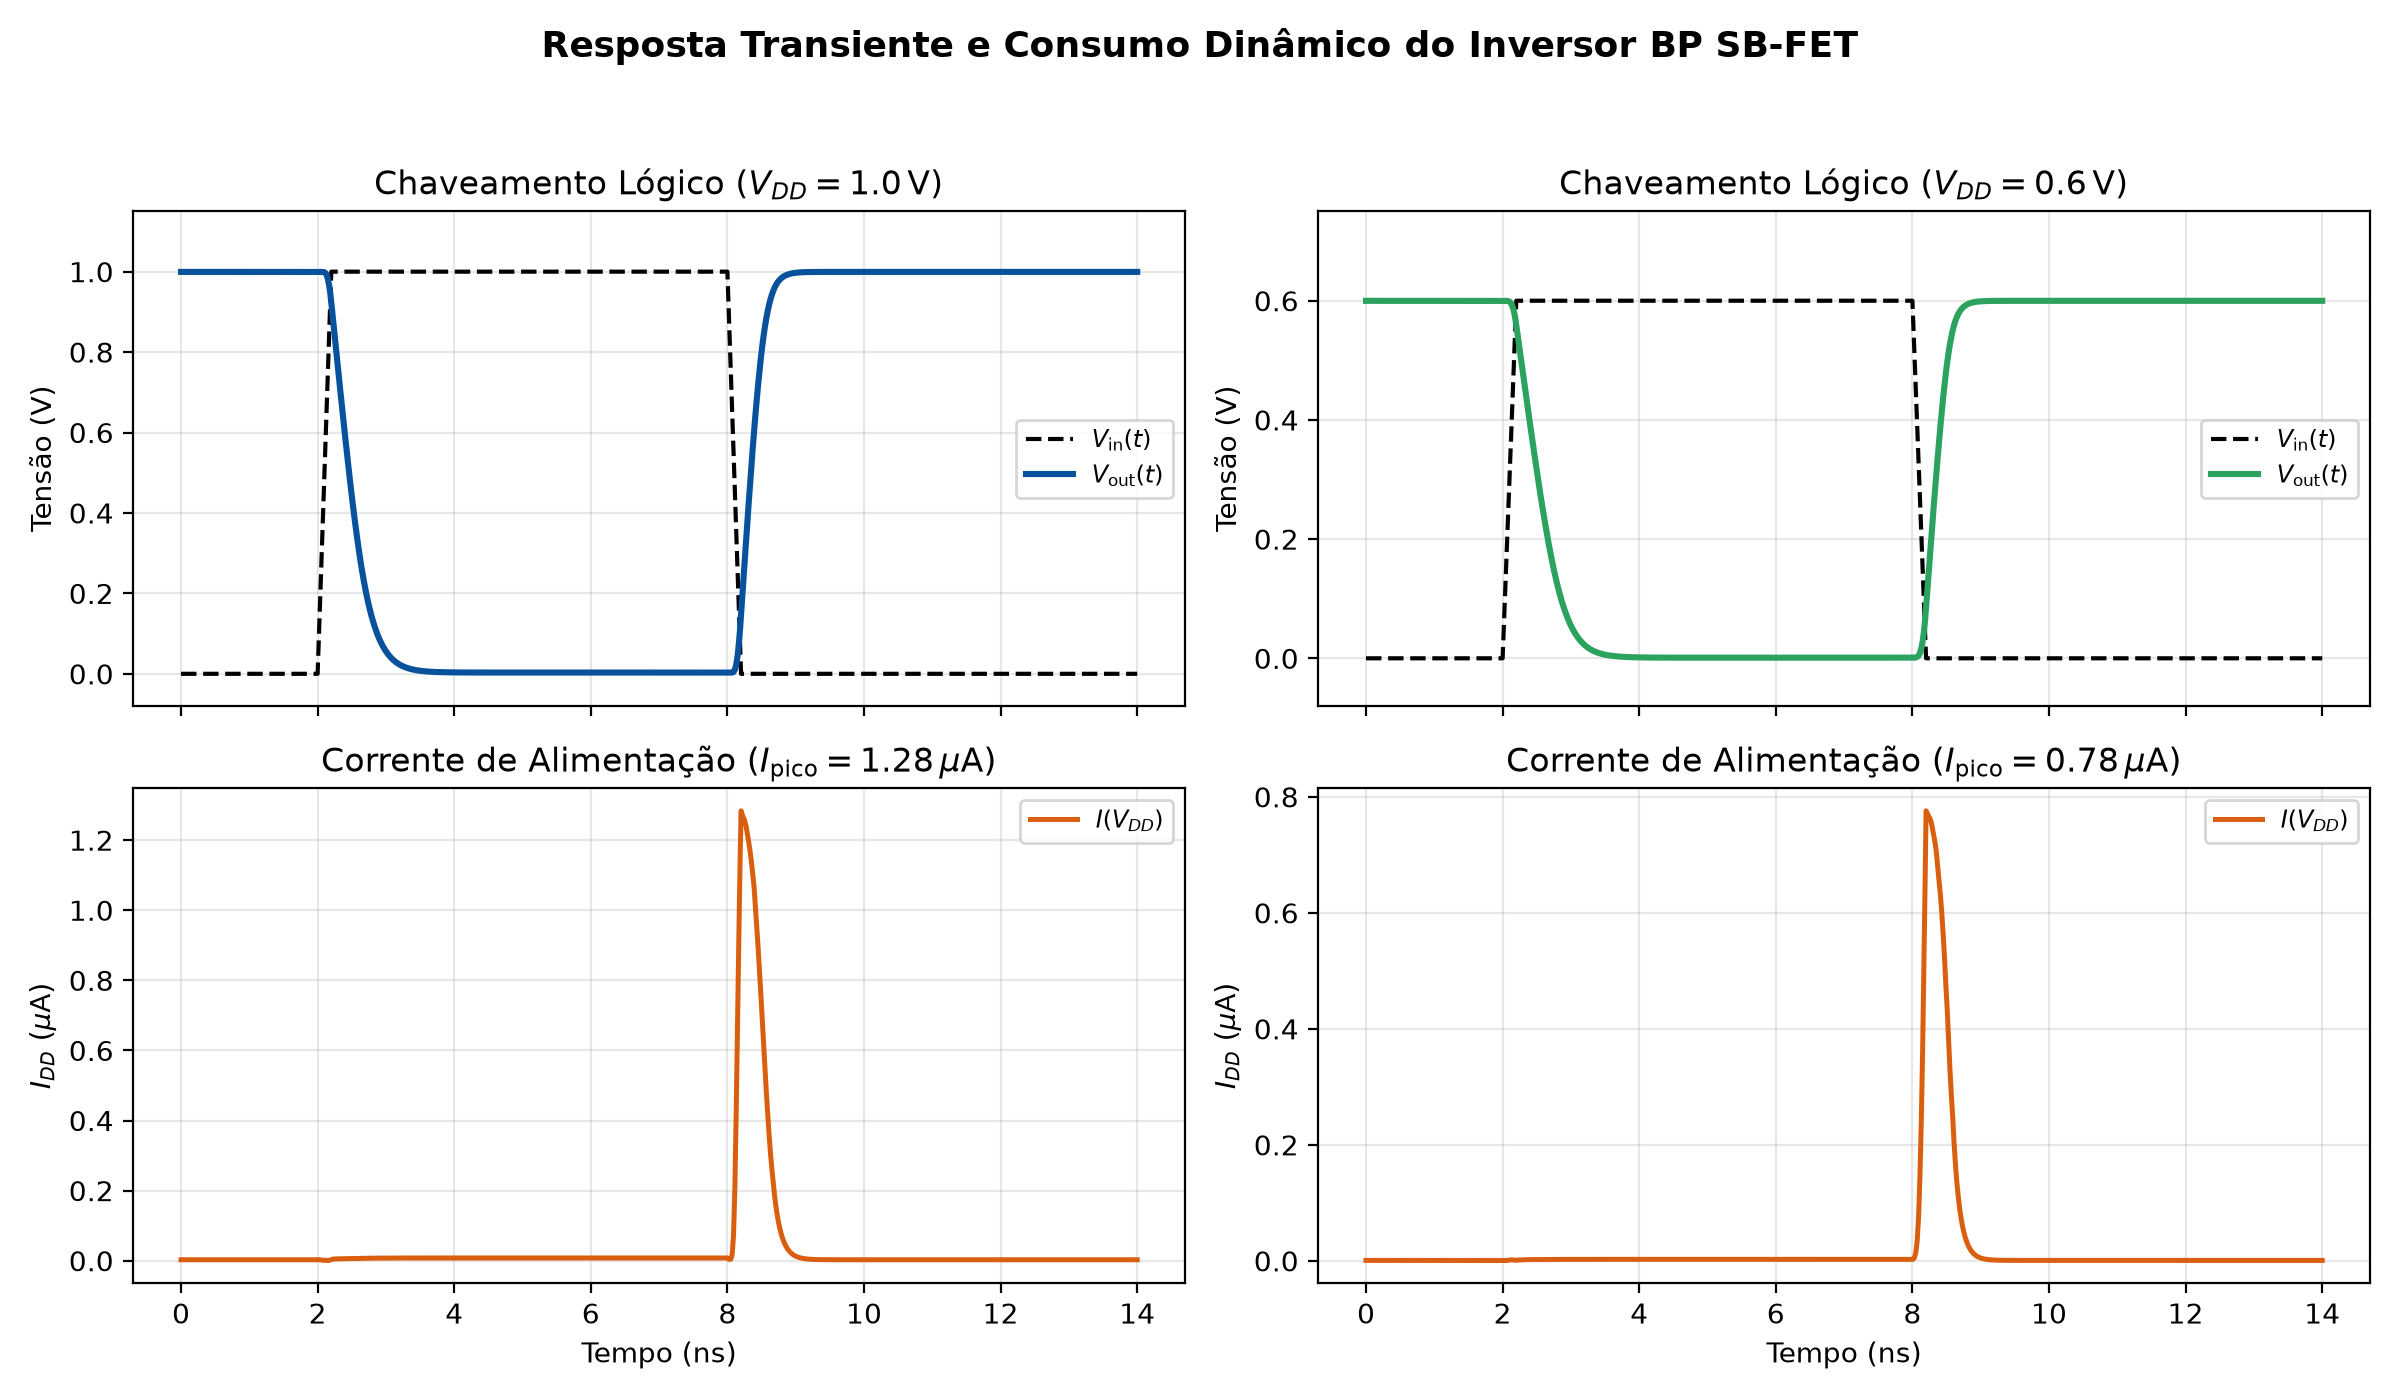
\includegraphics[width=0.90\textwidth]{m01_inversor_transiente.png}
\caption{Resposta transiente de chaveamento ($C_{\mathrm{load}} = 0{,}5\ \text{fF}$) e picos de corrente din\^{a}mica $I(V_{DD})$ do inversor compensado em $V_{DD} = 1{,}0\ \text{V}$ e $0{,}6\ \text{V}$.}
\label{fig:m01_tran}
\end{figure}

\subsection{Portas L\'{o}gicas Polim\'{o}rficas Din\^{a}micas (\texttt{NAND}/\texttt{NOR} e \texttt{XOR}/\texttt{XNOR})}\label{sec:res_poli}

As simula\c{c}\~{o}es transientes de $40\ \text{ns}$ comprovaram exatid\~{a}o booleana de $100\%$ ($16/16$ combina\c{c}\~{o}es de entrada e chave) em ambas as primitivas polim\'{o}rficas de 4 transistores sem sobrecarga de \'{a}rea, conforme detalhado na Tabela~\ref{tab:portas_polimorficas}. Na c\'{e}lula \texttt{NAND}/\texttt{NOR} ($V_{DD}=0{,}8\ \text{V}$), os n\'{i}veis l\'{o}gicos \texttt{'1'} situam-se entre $0{,}701\ \text{V}$ e $0{,}790\ \text{V}$, enquanto os n\'{i}veis \texttt{'0'} permanecem abaixo de $0{,}013\ \text{V}$. Na ponte \texttt{XOR}/\texttt{XNOR} ($V_{DD}=1{,}5\ \text{V}$, $V_{\mathrm{in}}=1{,}1\ \text{V}$), todos os estados \texttt{'1'} atingem exatamente $1{,}465\ \text{V}$ e todos os estados \texttt{'0'} estabilizam em $0{,}002\ \text{V}$.

\begin{table}[htbp]
\centering
\caption{Tabela-verdade el\'{e}trica e correntes de pico medidas no \texttt{ngspice-47} para as portas polim\'{o}rficas de 4T.}
\label{tab:portas_polimorficas}
\footnotesize
\begin{tabular}{l c c c c c c c}
\toprule
\textbf{Porta ($V_{DD}$)} & \textbf{Chave} & \textbf{Fun\c{c}\~{a}o} & $(A,B)$ & $V_{\mathrm{out}}$ (V) & \textbf{Bit Med.} & \textbf{Bit Esp.} & $I_{\mathrm{pico}}$ ($\mu\text{A}$) \\
\midrule
\texttt{NAND}/\texttt{NOR} ($0{,}8\ \text{V}$) & $\text{Key}=0$ & \texttt{NAND} & \texttt{00} & $0{,}790$ & \texttt{1} & \texttt{1} & $0{,}041$ \\
\texttt{NAND}/\texttt{NOR} ($0{,}8\ \text{V}$) & $\text{Key}=0$ & \texttt{NAND} & \texttt{01} & $0{,}762$ & \texttt{1} & \texttt{1} & $0{,}182$ \\
\texttt{NAND}/\texttt{NOR} ($0{,}8\ \text{V}$) & $\text{Key}=0$ & \texttt{NAND} & \texttt{10} & $0{,}769$ & \texttt{1} & \texttt{1} & $0{,}390$ \\
\texttt{NAND}/\texttt{NOR} ($0{,}8\ \text{V}$) & $\text{Key}=0$ & \texttt{NAND} & \texttt{11} & $0{,}013$ & \texttt{0} & \texttt{0} & $0{,}589$ \\
\texttt{NAND}/\texttt{NOR} ($0{,}8\ \text{V}$) & $\text{Key}=1$ & \texttt{NOR}  & \texttt{00} & $0{,}701$ & \texttt{1} & \texttt{1} & $0{,}213$ \\
\texttt{NAND}/\texttt{NOR} ($0{,}8\ \text{V}$) & $\text{Key}=1$ & \texttt{NOR}  & \texttt{01} & $0{,}001$ & \texttt{0} & \texttt{0} & $0{,}716$ \\
\texttt{NAND}/\texttt{NOR} ($0{,}8\ \text{V}$) & $\text{Key}=1$ & \texttt{NOR}  & \texttt{10} & $0{,}004$ & \texttt{0} & \texttt{0} & $0{,}092$ \\
\texttt{NAND}/\texttt{NOR} ($0{,}8\ \text{V}$) & $\text{Key}=1$ & \texttt{NOR}  & \texttt{11} & $0{,}001$ & \texttt{0} & \texttt{0} & $0{,}006$ \\
\midrule
\texttt{XOR}/\texttt{XNOR} ($1{,}5\ \text{V}$) & $\text{Key}=0$ & \texttt{XOR}  & \texttt{00} & $0{,}002$ & \texttt{0} & \texttt{0} & $0{,}004$ \\
\texttt{XOR}/\texttt{XNOR} ($1{,}5\ \text{V}$) & $\text{Key}=0$ & \texttt{XOR}  & \texttt{01} & $1{,}465$ & \texttt{1} & \texttt{1} & $1{,}691$ \\
\texttt{XOR}/\texttt{XNOR} ($1{,}5\ \text{V}$) & $\text{Key}=0$ & \texttt{XOR}  & \texttt{10} & $1{,}465$ & \texttt{1} & \texttt{1} & $0{,}366$ \\
\texttt{XOR}/\texttt{XNOR} ($1{,}5\ \text{V}$) & $\text{Key}=0$ & \texttt{XOR}  & \texttt{11} & $0{,}002$ & \texttt{0} & \texttt{0} & $1{,}903$ \\
\texttt{XOR}/\texttt{XNOR} ($1{,}5\ \text{V}$) & $\text{Key}=1$ & \texttt{XNOR} & \texttt{00} & $1{,}465$ & \texttt{1} & \texttt{1} & $1{,}699$ \\
\texttt{XOR}/\texttt{XNOR} ($1{,}5\ \text{V}$) & $\text{Key}=1$ & \texttt{XNOR} & \texttt{01} & $0{,}002$ & \texttt{0} & \texttt{0} & $1{,}908$ \\
\texttt{XOR}/\texttt{XNOR} ($1{,}5\ \text{V}$) & $\text{Key}=1$ & \texttt{XNOR} & \texttt{10} & $0{,}002$ & \texttt{0} & \texttt{0} & $0{,}032$ \\
\texttt{XOR}/\texttt{XNOR} ($1{,}5\ \text{V}$) & $\text{Key}=1$ & \texttt{XNOR} & \texttt{11} & $1{,}465$ & \texttt{1} & \texttt{1} & $1{,}691$ \\
\bottomrule
\end{tabular}
\end{table}

As Figuras~\ref{fig:m02_nand_nor} e \ref{fig:m02_xor_xnor} evidenciam a transmuta\c{c}\~{a}o instant\^{a}nea em $t = 20\ \text{ns}$ e exp\~{o}em uma diferen\c{c}a estrutural fundamental: enquanto \texttt{NAND}/\texttt{NOR} apresenta picos de corrente fortemente dependentes da rede s\'{e}rie ou paralela que realiza a transi\c{c}\~{a}o, a ponte \texttt{XOR}/\texttt{XNOR} exibe picos de carga ($\approx 1{,}69\ \mu\text{A}$) e descarga ($\approx 1{,}90\text{--}1{,}91\ \mu\text{A}$) praticamente espelhados entre os dois modos de chave.

\begin{figure}[htbp]
\centering
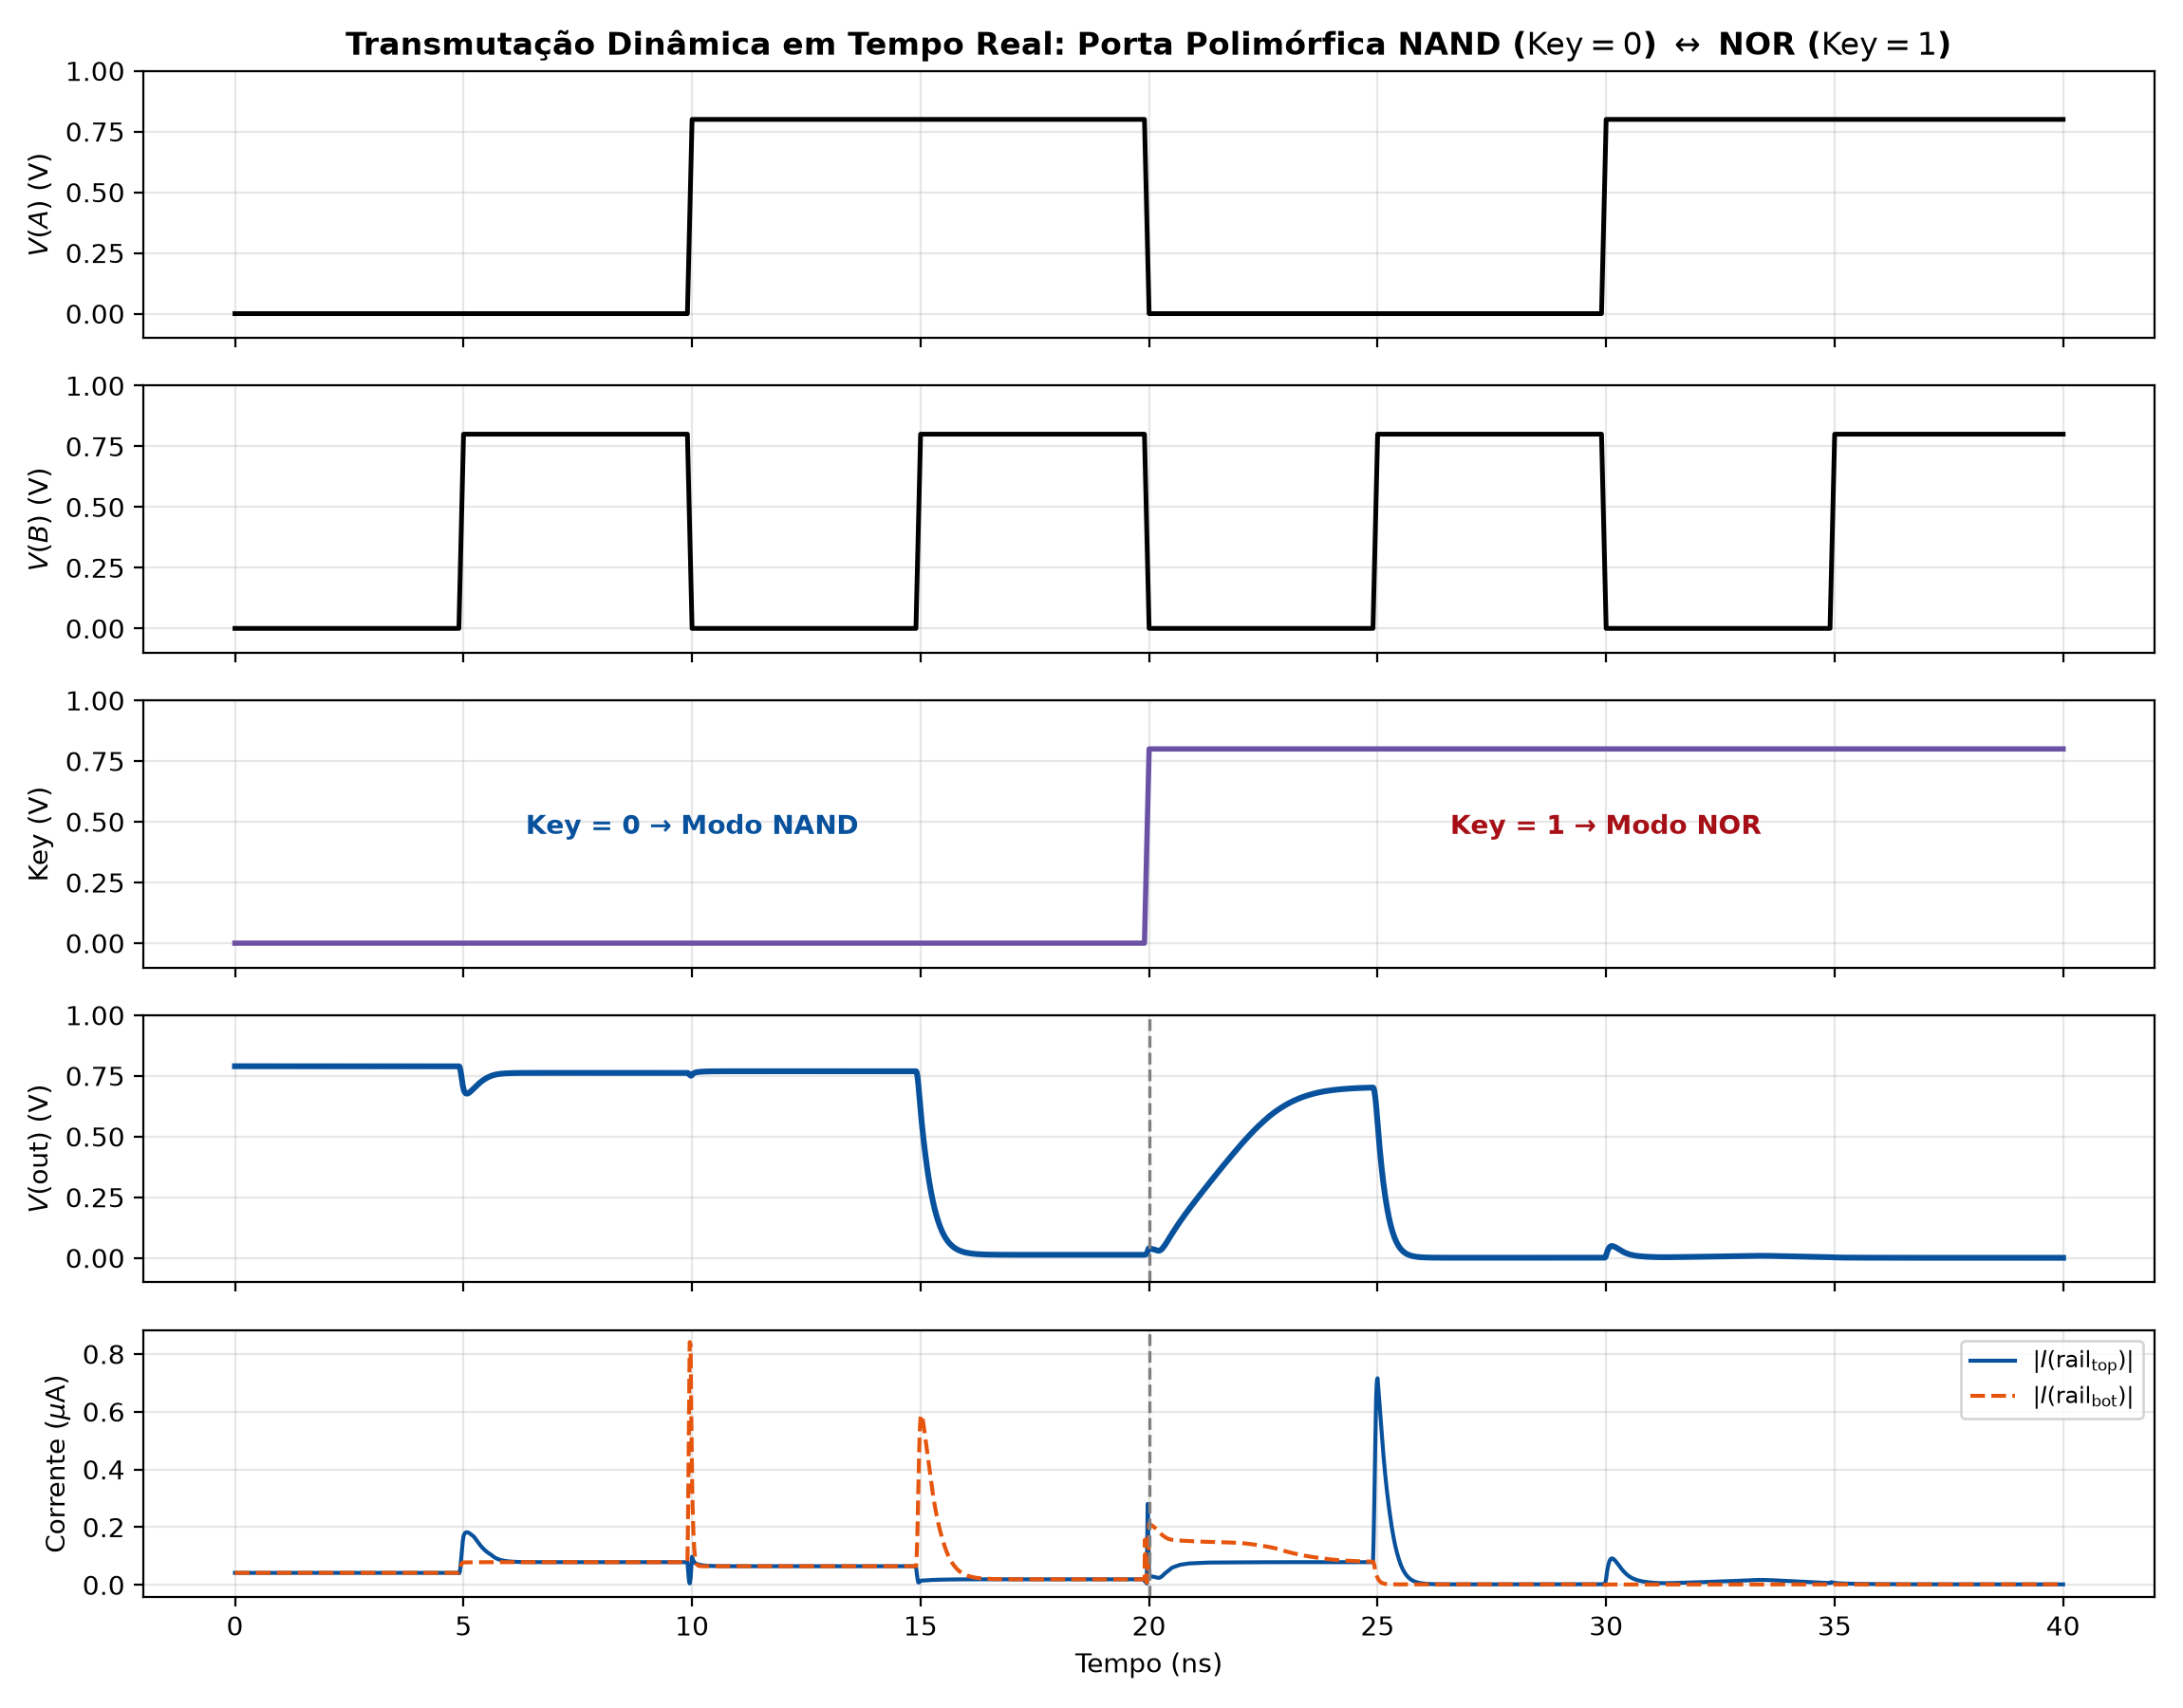
\includegraphics[width=0.90\textwidth]{m02_nand_nor_dinamico.png}
\caption{Comuta\c{c}\~{a}o din\^{a}mica \texttt{NAND} ($\text{Key}=0$) $\leftrightarrow$ \texttt{NOR} ($\text{Key}=1$) em $V_{DD} = 0{,}8\ \text{V}$ e perfil assim\'{e}trico da corrente de alimenta\c{c}\~{a}o.}
\label{fig:m02_nand_nor}
\end{figure}

\begin{figure}[htbp]
\centering
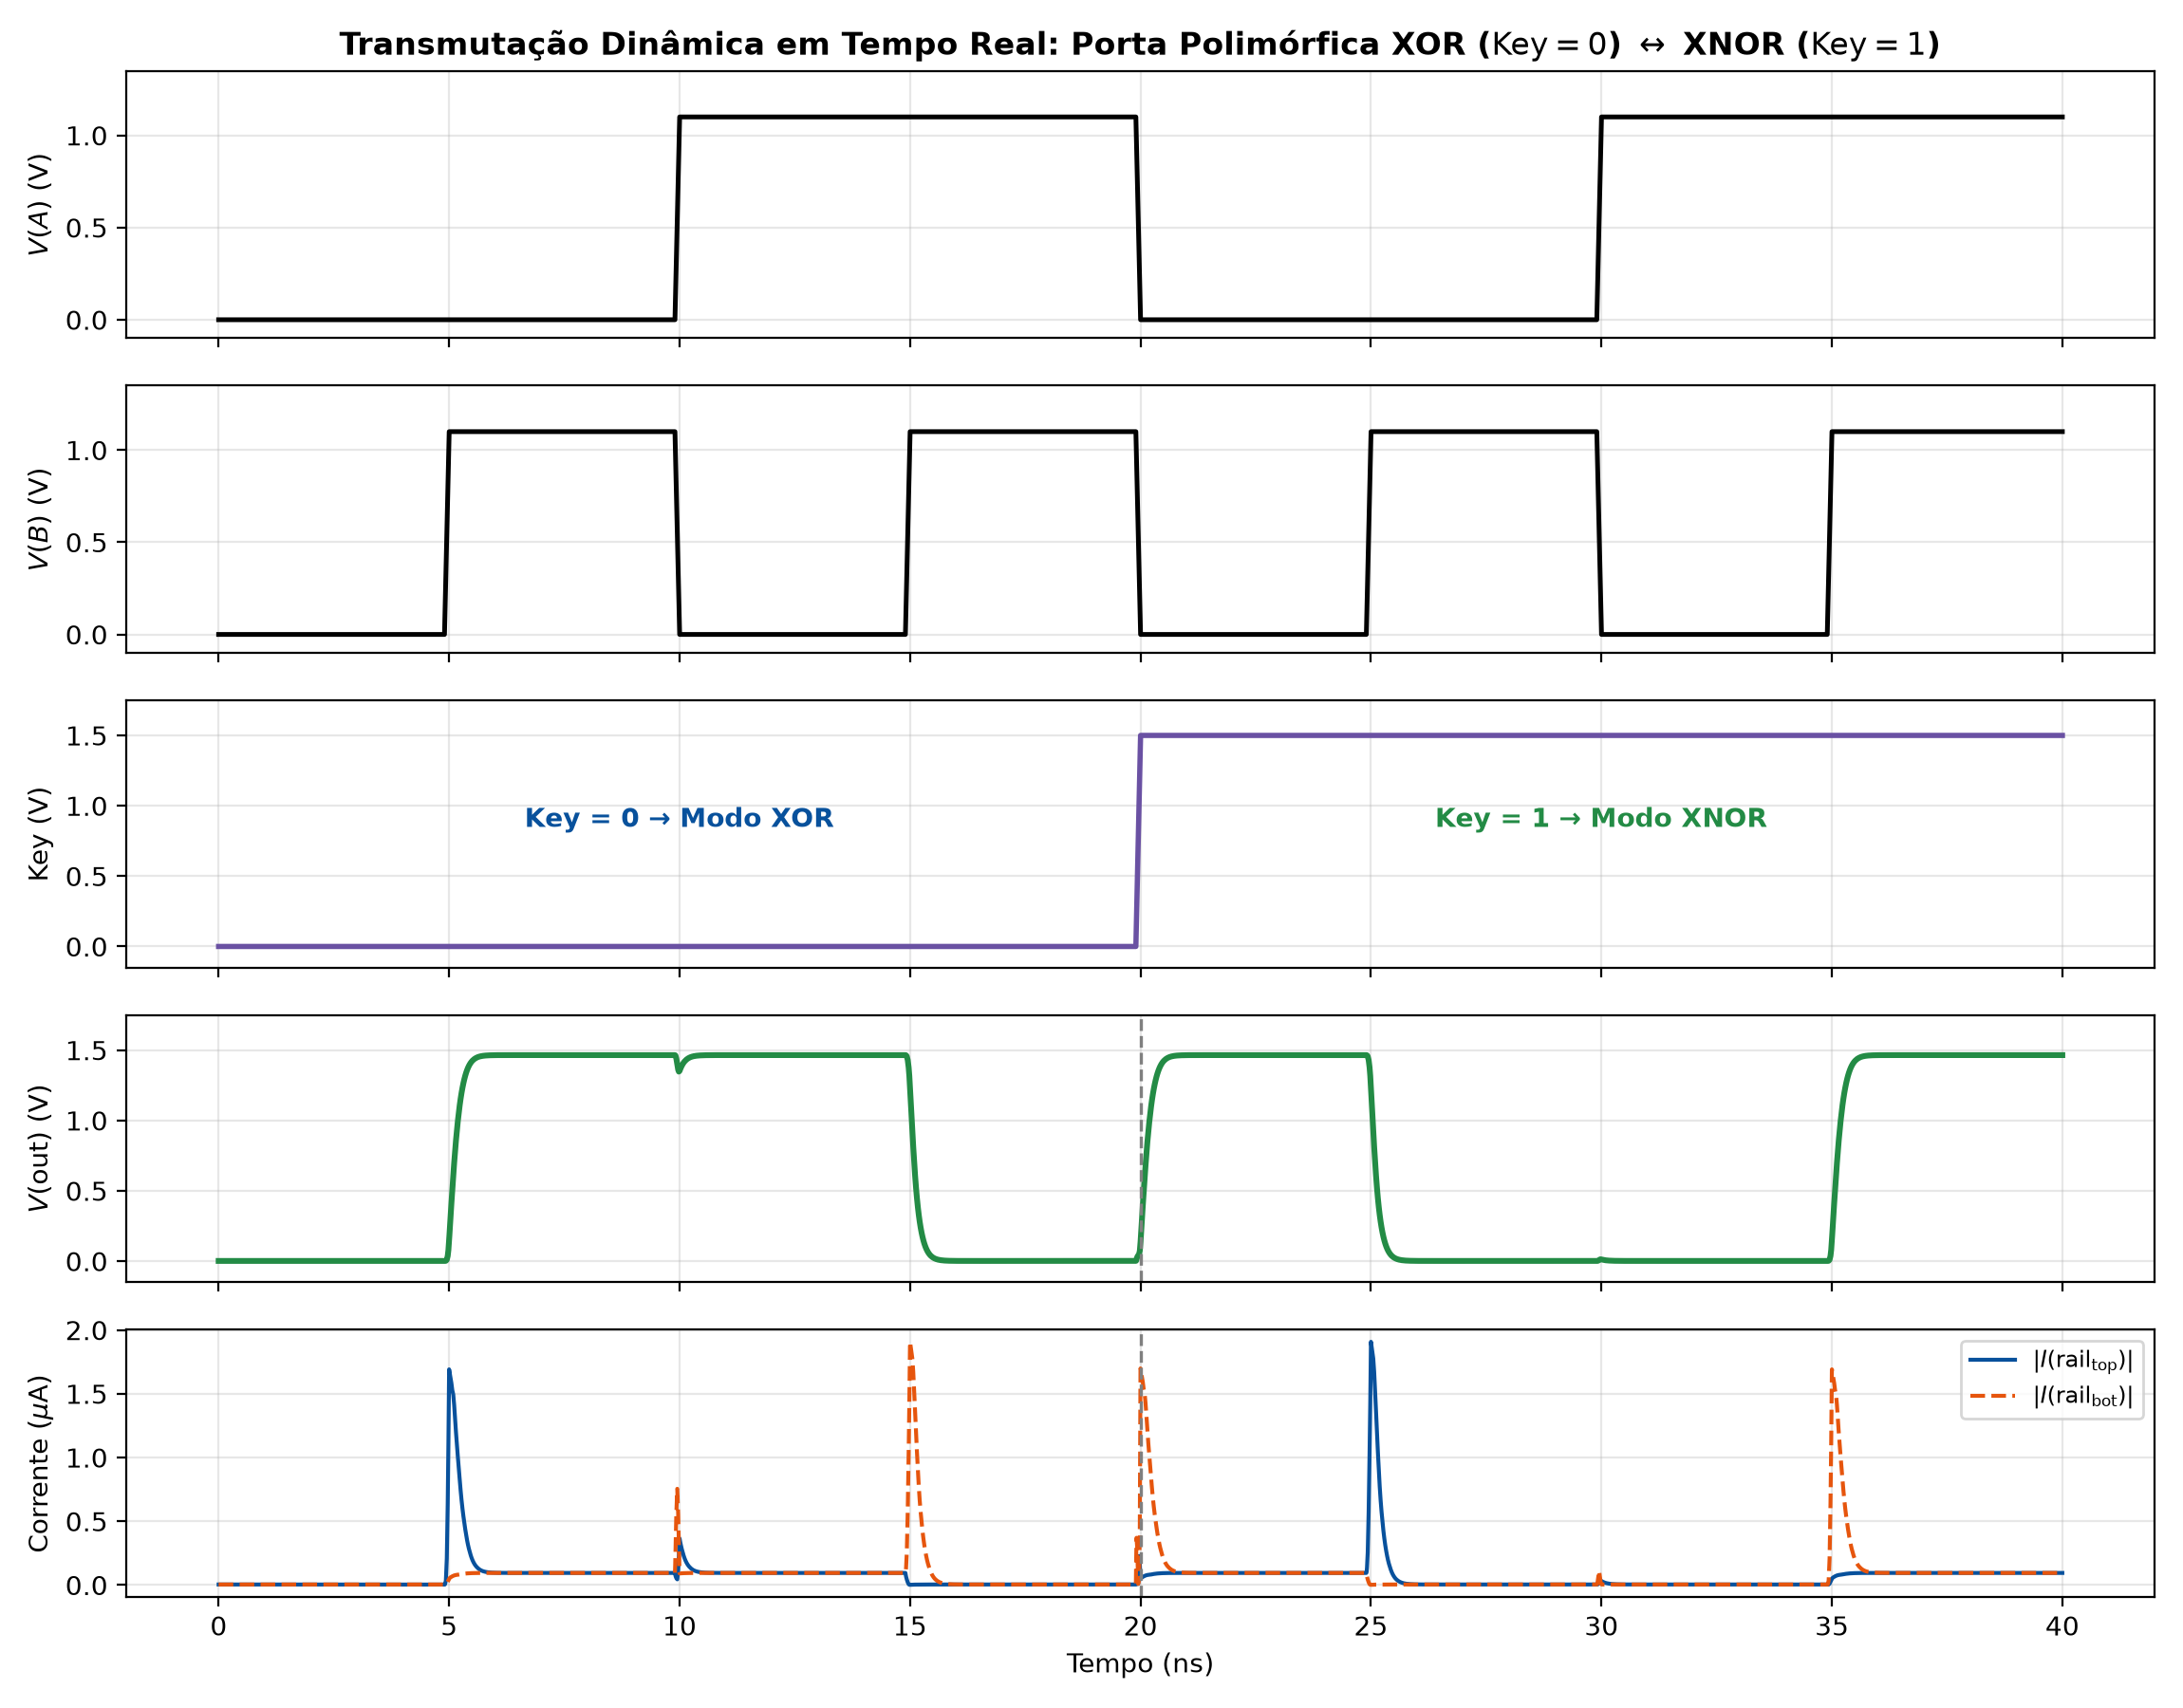
\includegraphics[width=0.90\textwidth]{m02_xor_xnor_dinamico.png}
\caption{Comuta\c{c}\~{a}o din\^{a}mica \texttt{XOR} ($\text{Key}=0$) $\leftrightarrow$ \texttt{XNOR} ($\text{Key}=1$) em $V_{DD} = 1{,}5\ \text{V}$ com simetria nos picos de chaveamento complementares.}
\label{fig:m02_xor_xnor}
\end{figure}

\subsection{Seguran\c{c}a contra Canal Lateral (DPA), Robustez 3D e Reten\c{c}\~{a}o Flutuante}\label{sec:res_dpa_mc}

A an\'{a}lise reproduzida em Python sobre as formas de onda experimentais de~\cite{wu2020reconfigurable} (Tabela~\ref{tab:dpa_mc_m03} e Figura~\ref{fig:m03_dpa}) confirma que a fam\'{i}lia \texttt{NAND}/\texttt{NOR} exibe uma discrep\^{a}ncia de $50{,}3\%$ nos picos de corrente ($2{,}15\ \mu\text{A}$ vs.\ $1{,}43\ \mu\text{A}$) e correla\c{c}\~{a}o temporal limitada ($r = 0{,}515$), enquanto a fam\'{i}lia \texttt{XOR}/\texttt{XNOR} reduz a diferen\c{c}a entre picos para apenas $0{,}56\%$ ($1{,}80\ \mu\text{A}$ vs.\ $1{,}79\ \mu\text{A}$), mascarando a identidade da chave sob monitoramento de canal lateral.

\begin{table}[htbp]
\centering
\caption{M\'{e}tricas de assinatura DPA e robustez estat\'{i}stica Monte Carlo ($N=250$ amostras/porta) do M\'{o}dulo \texttt{03}.}
\label{tab:dpa_mc_m03}
\begin{subtable}{\textwidth}
\centering
\caption{Compara\c{c}\~{a}o de assinaturas de corrente $|I(V_{DD})|$ entre modos (\texttt{metricas\_dpa.csv}).}
\footnotesize
\begin{tabular}{l c c c c c c}
\toprule
\textbf{Fam\'{i}lia} & $I_{\mathrm{pico},0}$ ($\mu\text{A}$) & $I_{\mathrm{pico},1}$ ($\mu\text{A}$) & \textbf{Dif.\ Pico (\%)} & $I_{\mathrm{m\acute{e}d},0}$ ($\mu\text{A}$) & $I_{\mathrm{m\acute{e}d},1}$ ($\mu\text{A}$) & \textbf{Correla\c{c}\~{a}o} $r$ \\
\midrule
\texttt{NAND}/\texttt{NOR} & $2{,}15$ & $1{,}43$ & $50{,}35\%$ & $0{,}212$ & $0{,}163$ & $+0{,}515$ \\
\texttt{XOR}/\texttt{XNOR} & $1{,}80$ & $1{,}79$ & $0{,}56\%$  & $0{,}267$ & $0{,}230$ & $-0{,}114$ \\
\bottomrule
\end{tabular}
\end{subtable}

\vspace{0.8em}

\begin{subtable}{\textwidth}
\centering
\caption{Estat\'{i}sticas de separa\c{c}\~{a}o l\'{o}gica sob ru\'{i}do simult\^{a}neo em $V_{DD}$ e $V_{SS}$ (\texttt{metricas\_seguranca\_robustez.csv}).}
\footnotesize
\begin{tabular}{l c c c c c c}
\toprule
\textbf{Porta} & \textbf{Amostras} & $\mu(V_{\text{`1'}})$ (V) & $\sigma(V_{\text{`1'}})$ (mV) & $\mu(V_{\text{`0'}})$ (V) & $\sigma(V_{\text{`0'}})$ (mV) & \textbf{Acerto L\'{o}gico} \\
\midrule
\texttt{NAND} & $250$ & $0{,}793$ & $126{,}55$ & $0{,}038$ & $106{,}50$ & $100{,}0\%$ \\
\texttt{NOR}  & $250$ & $0{,}770$ & $118{,}01$ & $0{,}015$ & $101{,}47$ & $100{,}0\%$ \\
\texttt{XOR}  & $250$ & $0{,}782$ & $122{,}80$ & $0{,}006$ & $89{,}23$  & $100{,}0\%$ \\
\texttt{XNOR} & $250$ & $0{,}782$ & $122{,}69$ & $0{,}006$ & $89{,}05$  & $100{,}0\%$ \\
\bottomrule
\end{tabular}
\end{subtable}
\end{table}

\begin{figure}[htbp]
\centering
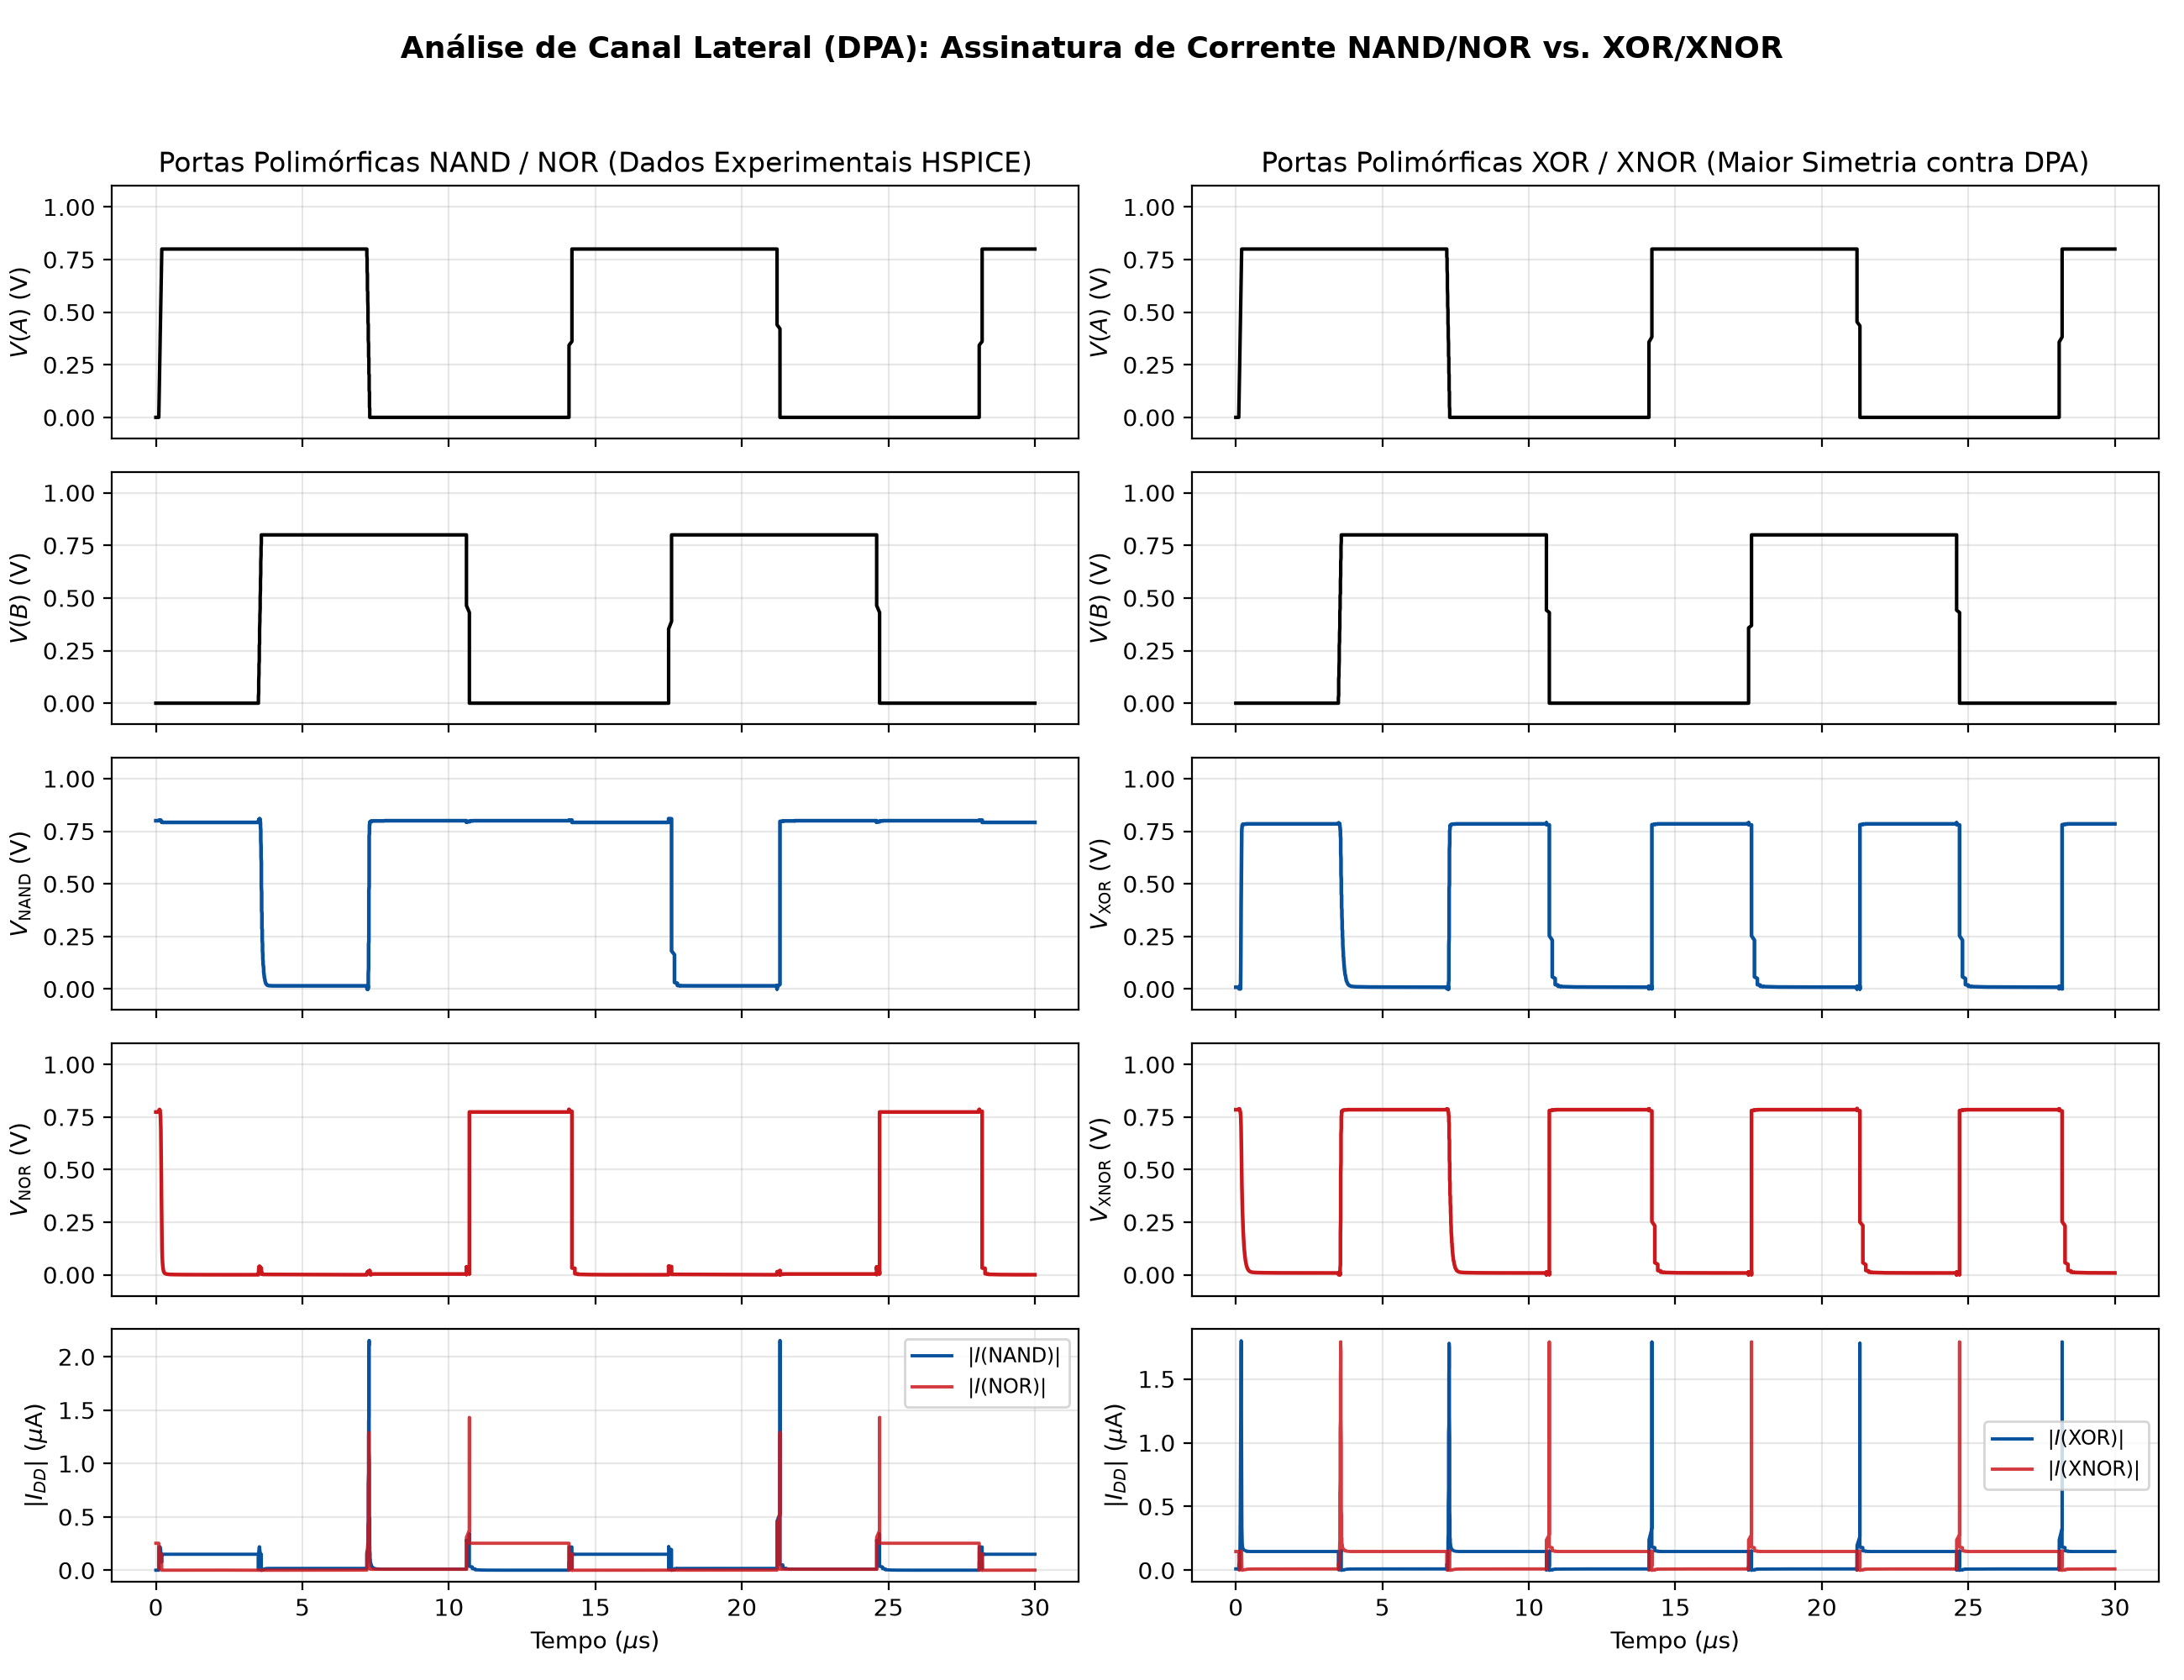
\includegraphics[width=0.92\textwidth]{m03_dpa_assinatura_corrente.png}
\caption{Comparativo de assinaturas de corrente $|I_{DD}|$ para ataque DPA entre \texttt{NAND}/\texttt{NOR} (esquerda) e \texttt{XOR}/\texttt{XNOR} (direita).}
\label{fig:m03_dpa}
\end{figure}

Nas 250 amostras de Monte Carlo (Figura~\ref{fig:m03_mc3d}), mesmo sob varia\c{c}\~{o}es severas nos trilhos ($V_{DD} \in [0{,}47;\ 1{,}15]\ \text{V}$), todas as quatro c\'{e}lulas atingiram $100{,}0\%$ de acerto l\'{o}gico sem sobreposi\c{c}\~{a}o entre os n\'{i}veis \texttt{'0'} e \texttt{'1'} em torno de $0{,}40\ \text{V}$. A valida\c{c}\~{a}o cruzada na grade $5 \times 5$ do \texttt{ngspice-47} (\texttt{ngspice\_supply\_sweep.csv}, Figura~\ref{fig:m03_hist_ret}) mostrou margem est\'{a}tica $(V_{00} - V_{11})$ entre $0{,}531\ \text{V}$ e $1{,}012\ \text{V}$ para $V_{DD} \ge 0{,}725\ \text{V}$ ou $V_{SS} \ge -0{,}05\ \text{V}$, degradando-se apenas no canto extremo ($V_{DD}=0{,}65\ \text{V},\ V_{SS}=-0{,}10\ \text{V}$), onde a margem cai para $0{,}153\ \text{V}$ ($V_{00} = 0{,}060\ \text{V}$ e $V_{11} = -0{,}093\ \text{V}$). Quanto \`{a} estabilidade temporal em n\'{o} flutuante (\texttt{bblc1}), ap\'{o}s os pulsos de excita\c{c}\~{a}o em $40$ e $80\ \mu\text{s}$, o potencial estabilizou em patamares distintos de $0{,}65\ \text{V}$ ($100\ \text{ns}$), $0{,}30\ \text{V}$ ($250\ \text{ns}$) e $0{,}20\ \text{V}$ ($500\ \text{ns}$) at\'{e} $111\ \mu\text{s}$.

\begin{figure}[htbp]
\centering
\begin{subfigure}{\textwidth}
  \centering
  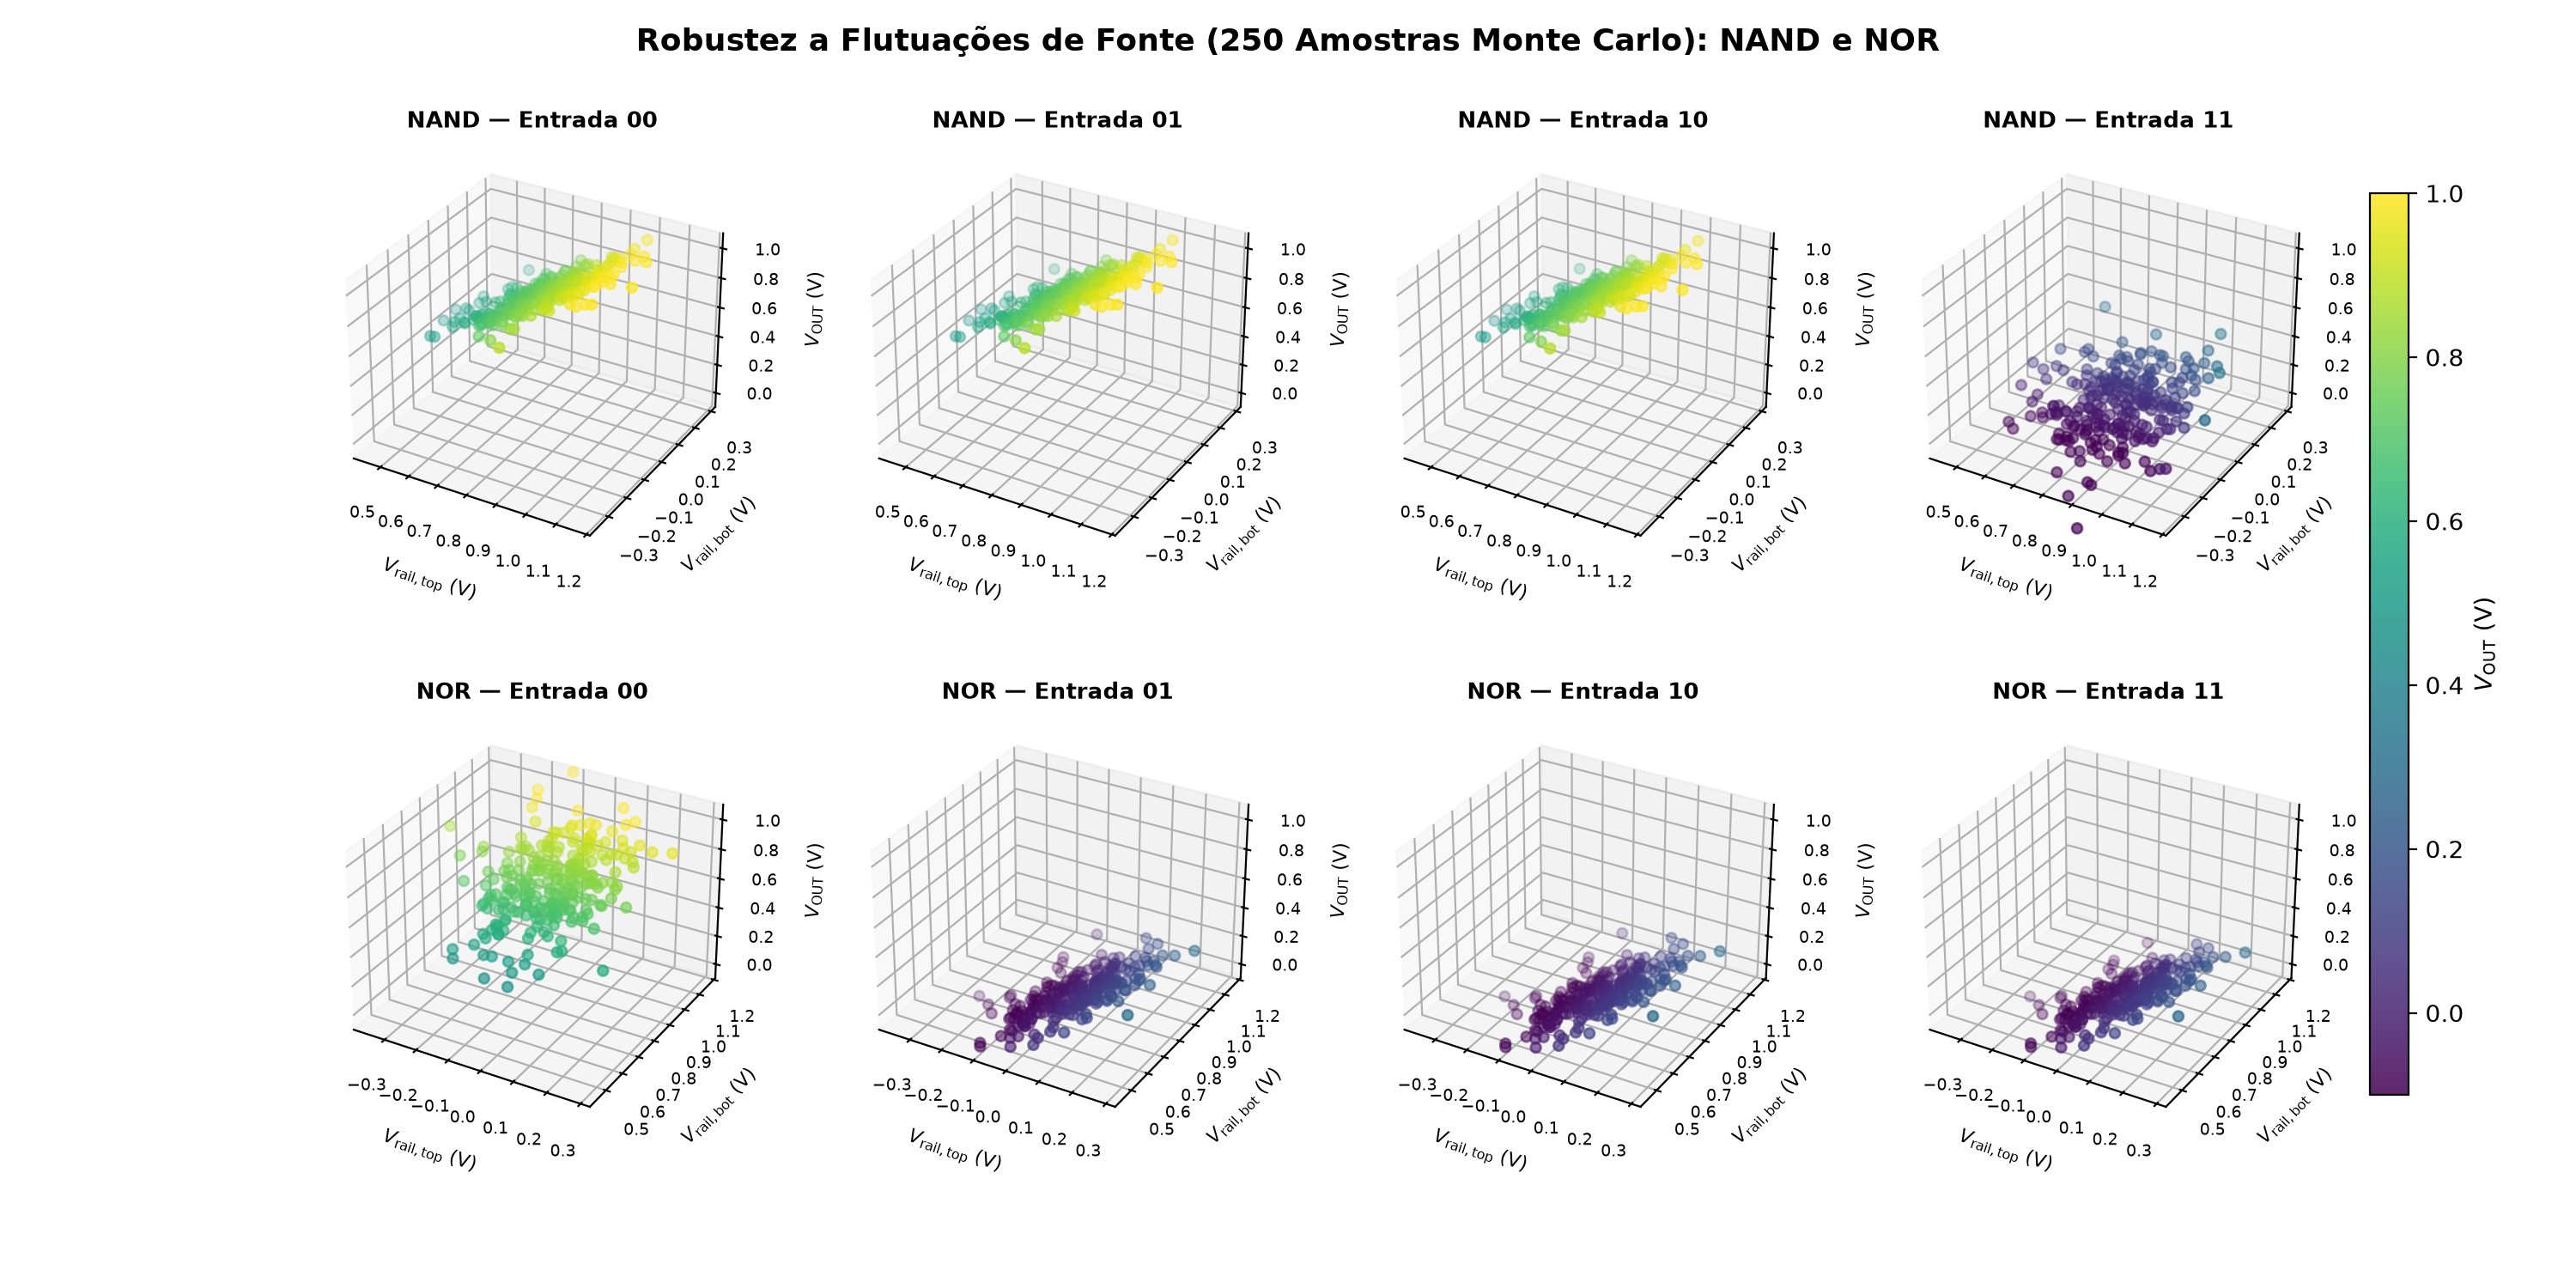
\includegraphics[width=0.95\textwidth]{m03_robustez_3d_nand_nor.png}
  \caption{Portas \texttt{NAND} e \texttt{NOR}.}
  \label{fig:m03_3d_nn}
\end{subfigure}
\par\medskip
\begin{subfigure}{\textwidth}
  \centering
  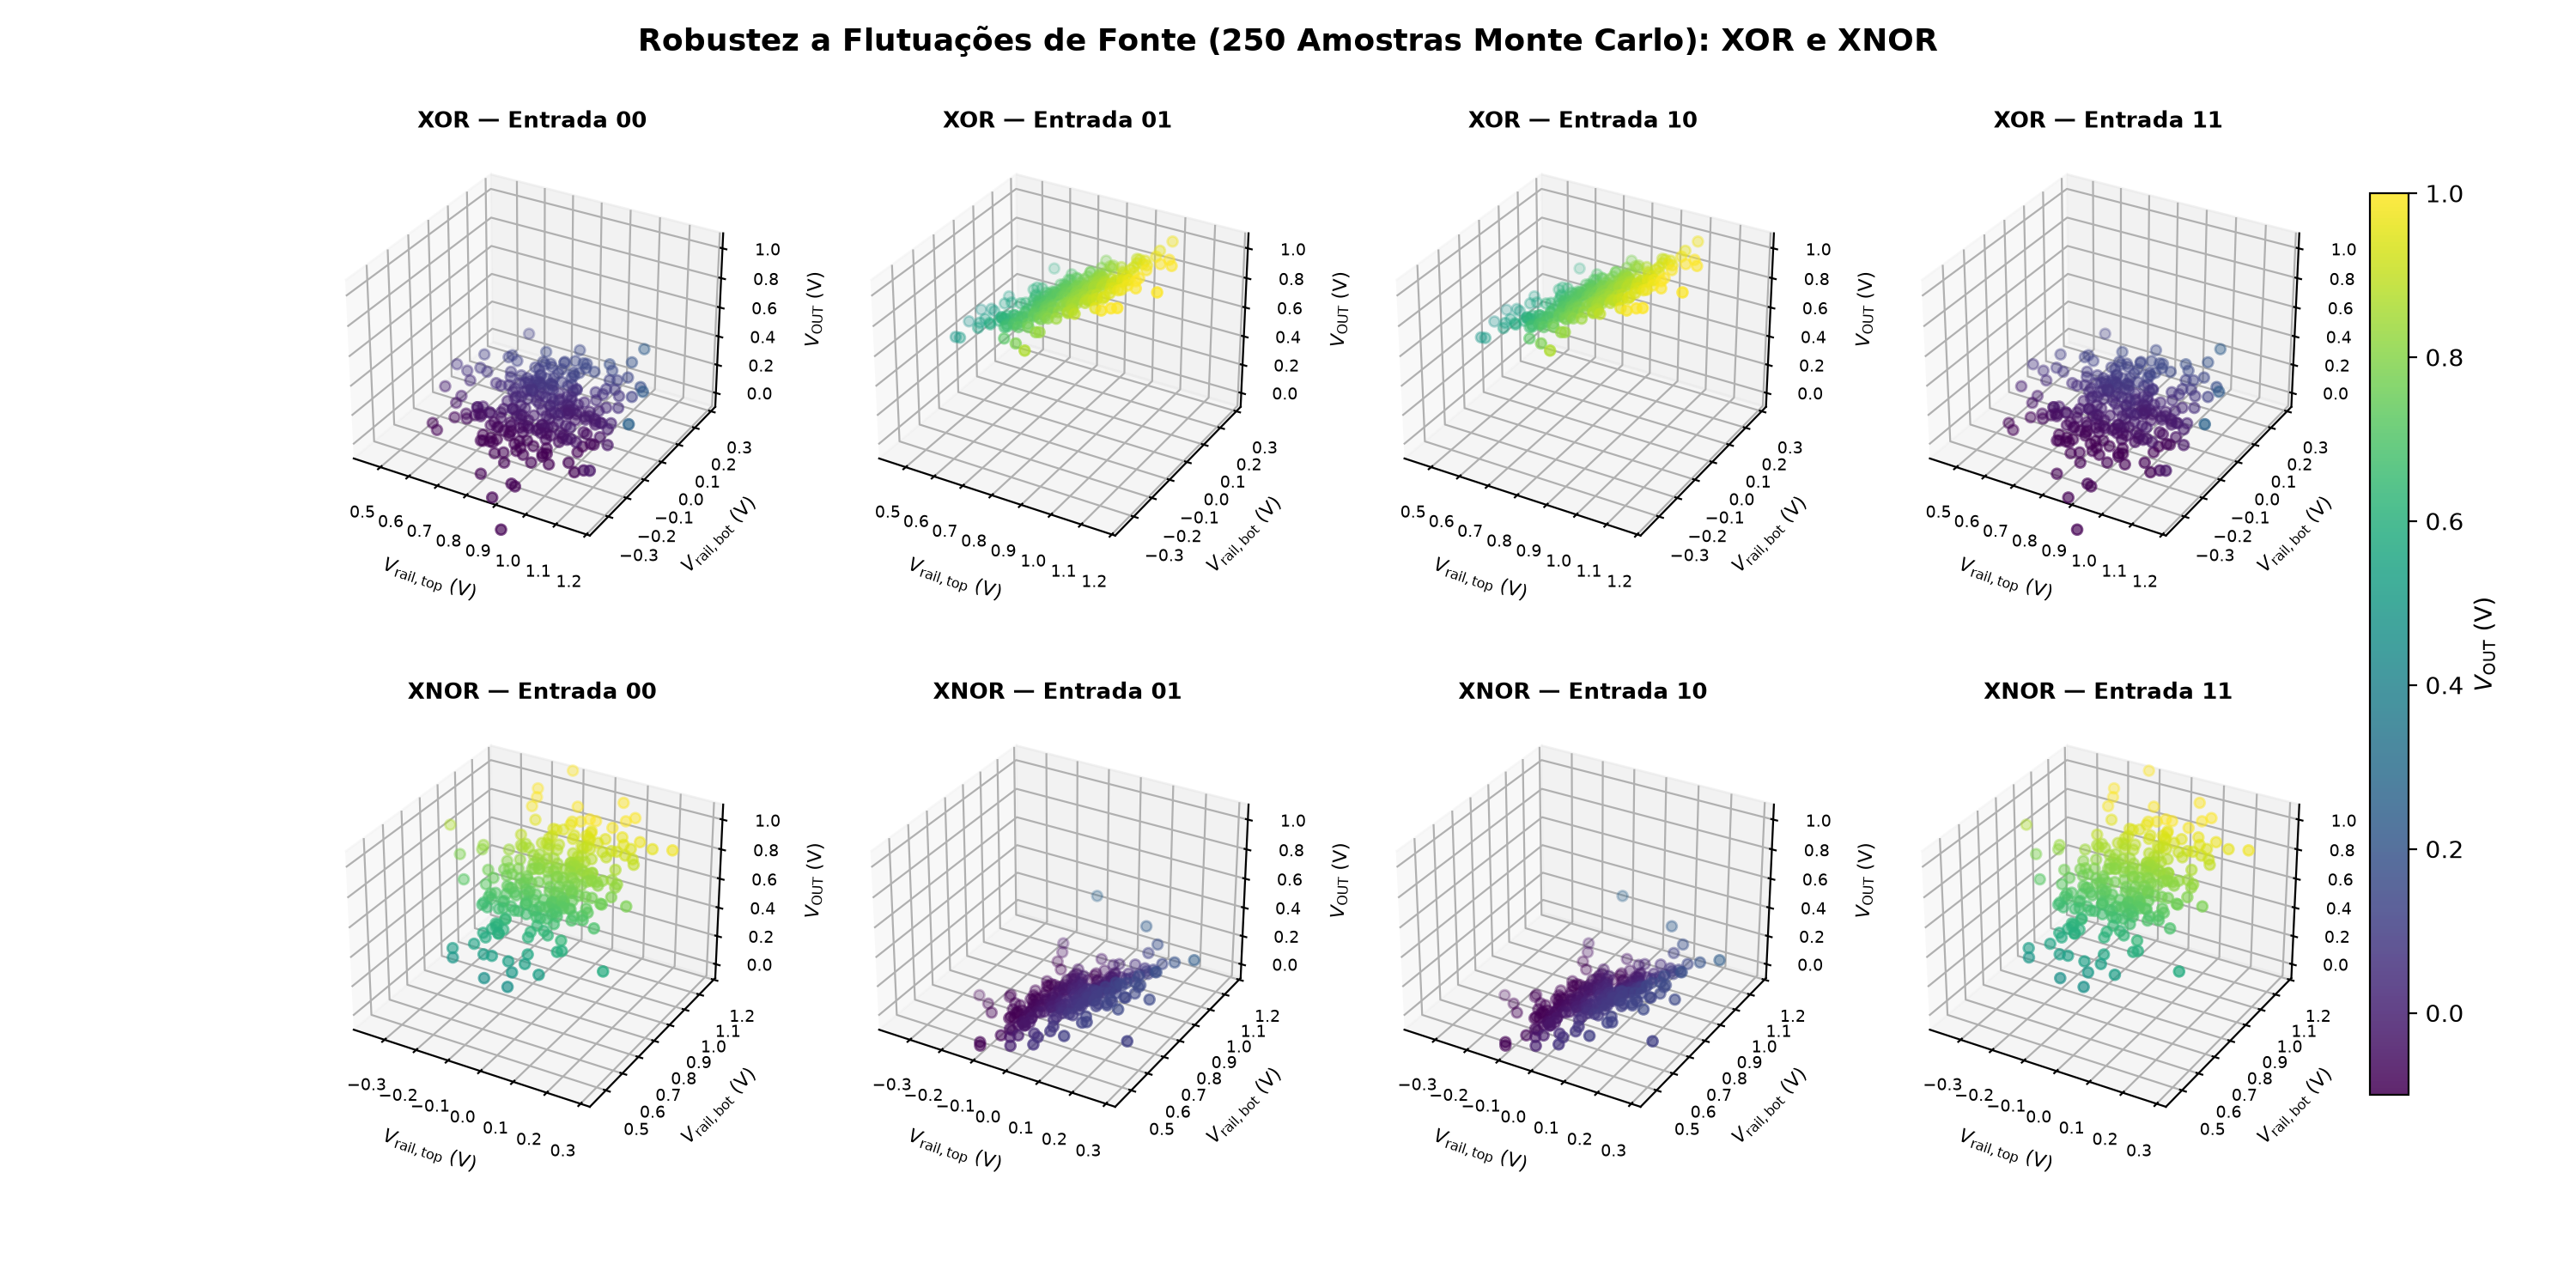
\includegraphics[width=0.95\textwidth]{m03_robustez_3d_xor_xnor.png}
  \caption{Portas \texttt{XOR} e \texttt{XNOR}.}
  \label{fig:m03_3d_xx}
\end{subfigure}
\caption{Superf\'{i}cies 3D de robustez ($V_{\mathrm{rail,top}} \times V_{\mathrm{rail,bot}} \times V_{\mathrm{OUT}}$) em 250 amostras Monte Carlo por vetor de entrada.}
\label{fig:m03_mc3d}
\end{figure}

\begin{figure}[htbp]
\centering
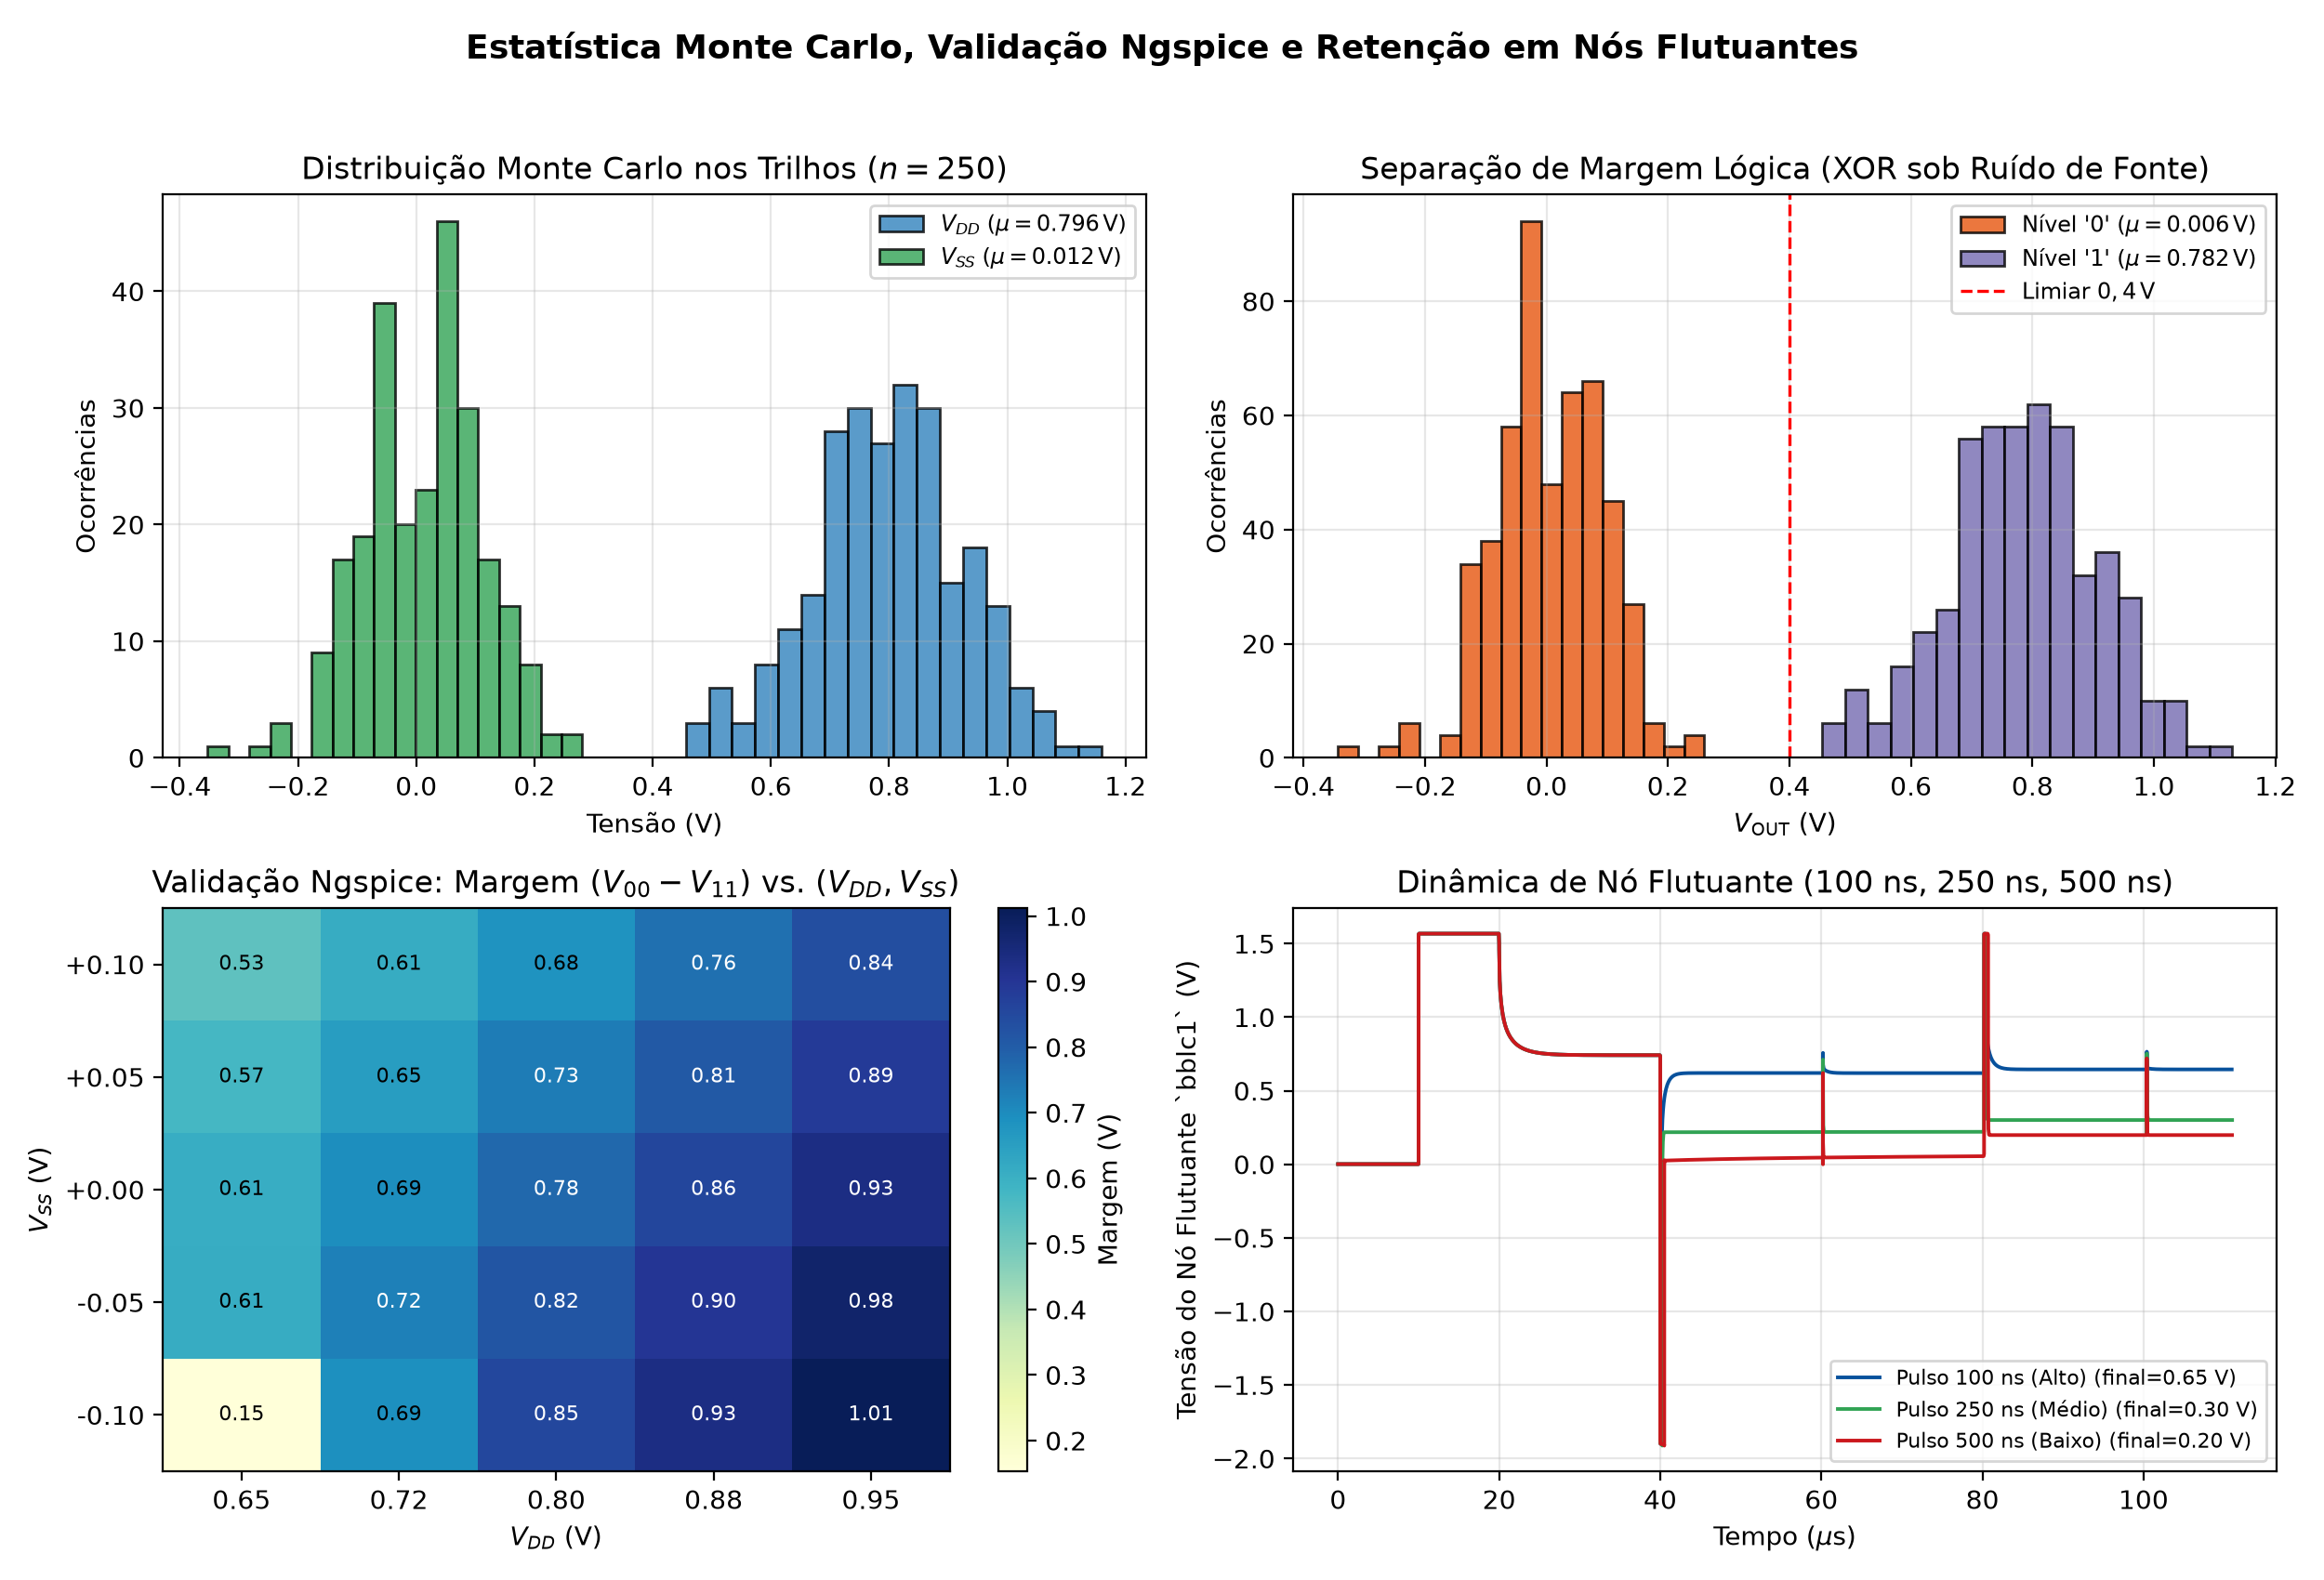
\includegraphics[width=0.92\textwidth]{m03_histogramas_e_retencao.png}
\caption{Distribui\c{c}\~{a}o Monte Carlo nos trilhos (superior esq.), separa\c{c}\~{a}o l\'{o}gica da \texttt{XOR} (superior dir.), mapa de margem $V_{DD}\times V_{SS}$ no \texttt{ngspice-47} (inferior esq.) e reten\c{c}\~{a}o em n\'{o} flutuante \texttt{bblc1} at\'{e} $111\ \mu\text{s}$ (inferior dir.).}
\label{fig:m03_hist_ret}
\end{figure}

\subsection{C\'{e}lula SRAM 6T com Bloqueio de Reten\c{c}\~{a}o (Mecanismo B)}\label{sec:res_sram}

A c\'{e}lula SRAM 6T satisfez todos os onze crit\'{e}rios de valida\c{c}\~{a}o transientes e est\'{a}ticos previstos para o Mecanismo B, conforme apresentado na Tabela~\ref{tab:sram_resultados}. Durante a simula\c{c}\~{a}o transiente de $30\ \text{ns}$ (Figura~\ref{fig:m04_tran}), sob $\text{Key} = 0$, a escrita do bit \texttt{'1'} ($0\text{--}6\ \text{ns}$) \'{e} retida ap\'{o}s o fechamento da \textit{Wordline} com $V(q) = 0{,}9768\ \text{V}$ e $V(qb) = 0{,}0020\ \text{V}$ em $t=12\ \text{ns}$ ($\Delta V_{\mathrm{Key0}} = 0{,}9747\ \text{V} > 0{,}80\ \text{V}$). No instante em que $\text{Key}$ comuta para $1$ ($t = 15\ \text{ns}$), mantendo $V_{DD} = 1{,}0\ \text{V}$ e $V_{SS} = 0{,}0\ \text{V}$ inalterados, a invers\~{a}o simult\^{a}nea das redes \textit{pull-up} (\textit{p-FET} $\to$ \textit{n-FET}) e \textit{pull-down} (\textit{n-FET} $\to$ \textit{p-FET}) provoca o colapso imediato do dado armazenado ($\Delta V_{\mathrm{Collapse1}} = 0{,}0841\ \text{V} < 0{,}15\ \text{V}$ em $18\ \text{ns}$). Na Fase 4 ($20\text{--}30\ \text{ns}$), mesmo for\c{c}ando o bit oposto durante o pulso de $\mathrm{WL}$, a c\'{e}lula volta a colapsar assim que $\mathrm{WL}$ fecha ($\Delta V_{\mathrm{Key1}} = 0{,}0762\ \text{V}$ em $28\ \text{ns}$).

\begin{table}[htbp]
\centering
\caption{M\'{e}tricas transientes ($30\ \text{ns}$) e margens est\'{a}ticas de ru\'{i}do (SNM) da c\'{e}lula SRAM 6T (\texttt{metricas\_sram\_6t.csv}).}
\label{tab:sram_resultados}
\footnotesize
\begin{tabular}{l c c c}
\toprule
\textbf{M\'{e}trica Extra\'{i}da} & \textbf{Valor Simulado} & \textbf{Crit\'{e}rio de Aceita\c{c}\~{a}o} & \textbf{Estado} \\
\midrule
$V(q)_{\mathrm{Hold}}$ ($\text{Key}=0,\ t=12\ \text{ns}$)   & $0{,}9768\ \text{V}$ & $> 0{,}80\ \text{V}$ & Aprovado \\
$V(qb)_{\mathrm{Hold}}$ ($\text{Key}=0,\ t=12\ \text{ns}$)  & $0{,}0020\ \text{V}$ & $< 0{,}20\ \text{V}$ & Aprovado \\
$\Delta V_{\mathrm{Key0}}$ ($t=12\ \text{ns}$)              & $0{,}9747\ \text{V}$ & $> 0{,}80\ \text{V}$ & Aprovado \\
$\Delta V_{\mathrm{Collapse1}}$ ($t=18\ \text{ns}$)         & $0{,}0841\ \text{V}$ & $< 0{,}15\ \text{V}$ & Aprovado \\
$\Delta V_{\mathrm{Key1}}$ ($t=28\ \text{ns}$)              & $0{,}0762\ \text{V}$ & $< 0{,}15\ \text{V}$ & Aprovado \\
$\mathrm{SNM}_{\mathrm{Hold}}$ ($\text{Key}=0,\ \mathrm{WL}=0\ \text{V}$)           & $167{,}12\ \text{mV}$ & $> 150\ \text{mV}$ & Aprovado \\
$\mathrm{SNM}_{\mathrm{Read,Unassisted}}$ ($\text{Key}=0,\ \mathrm{WL}=1{,}0\ \text{V}$) & $0{,}00\ \text{mV}$ & $0\ \text{mV}$ (\textit{Read Disturb}) & Diagnosticado \\
$\mathrm{SNM}_{\mathrm{Read,Assist}}$ ($\text{Key}=0,\ \mathrm{WL}=0{,}30\ \text{V}$) & $66{,}23\ \text{mV}$ & $> 50\ \text{mV}$ & Aprovado \\
$\mathrm{SNM}_{\mathrm{Hold}}$ ($\text{Key}=1,\ \mathrm{WL}=0\ \text{V}$)           & $0{,}00\ \text{mV}$ & $= 0\ \text{mV}$ & Aprovado \\
$\mathrm{SNM}_{\mathrm{Read,Assist}}$ ($\text{Key}=1,\ \mathrm{WL}=0{,}30\ \text{V}$) & $0{,}00\ \text{mV}$ & $= 0\ \text{mV}$ & Aprovado \\
$\mathrm{SNM}_{\mathrm{Read,Unassisted}}$ ($\text{Key}=1,\ \mathrm{WL}=1{,}0\ \text{V}$) & $0{,}00\ \text{mV}$ & $= 0\ \text{mV}$ & Aprovado \\
\bottomrule
\end{tabular}
\end{table}

\begin{figure}[htbp]
\centering
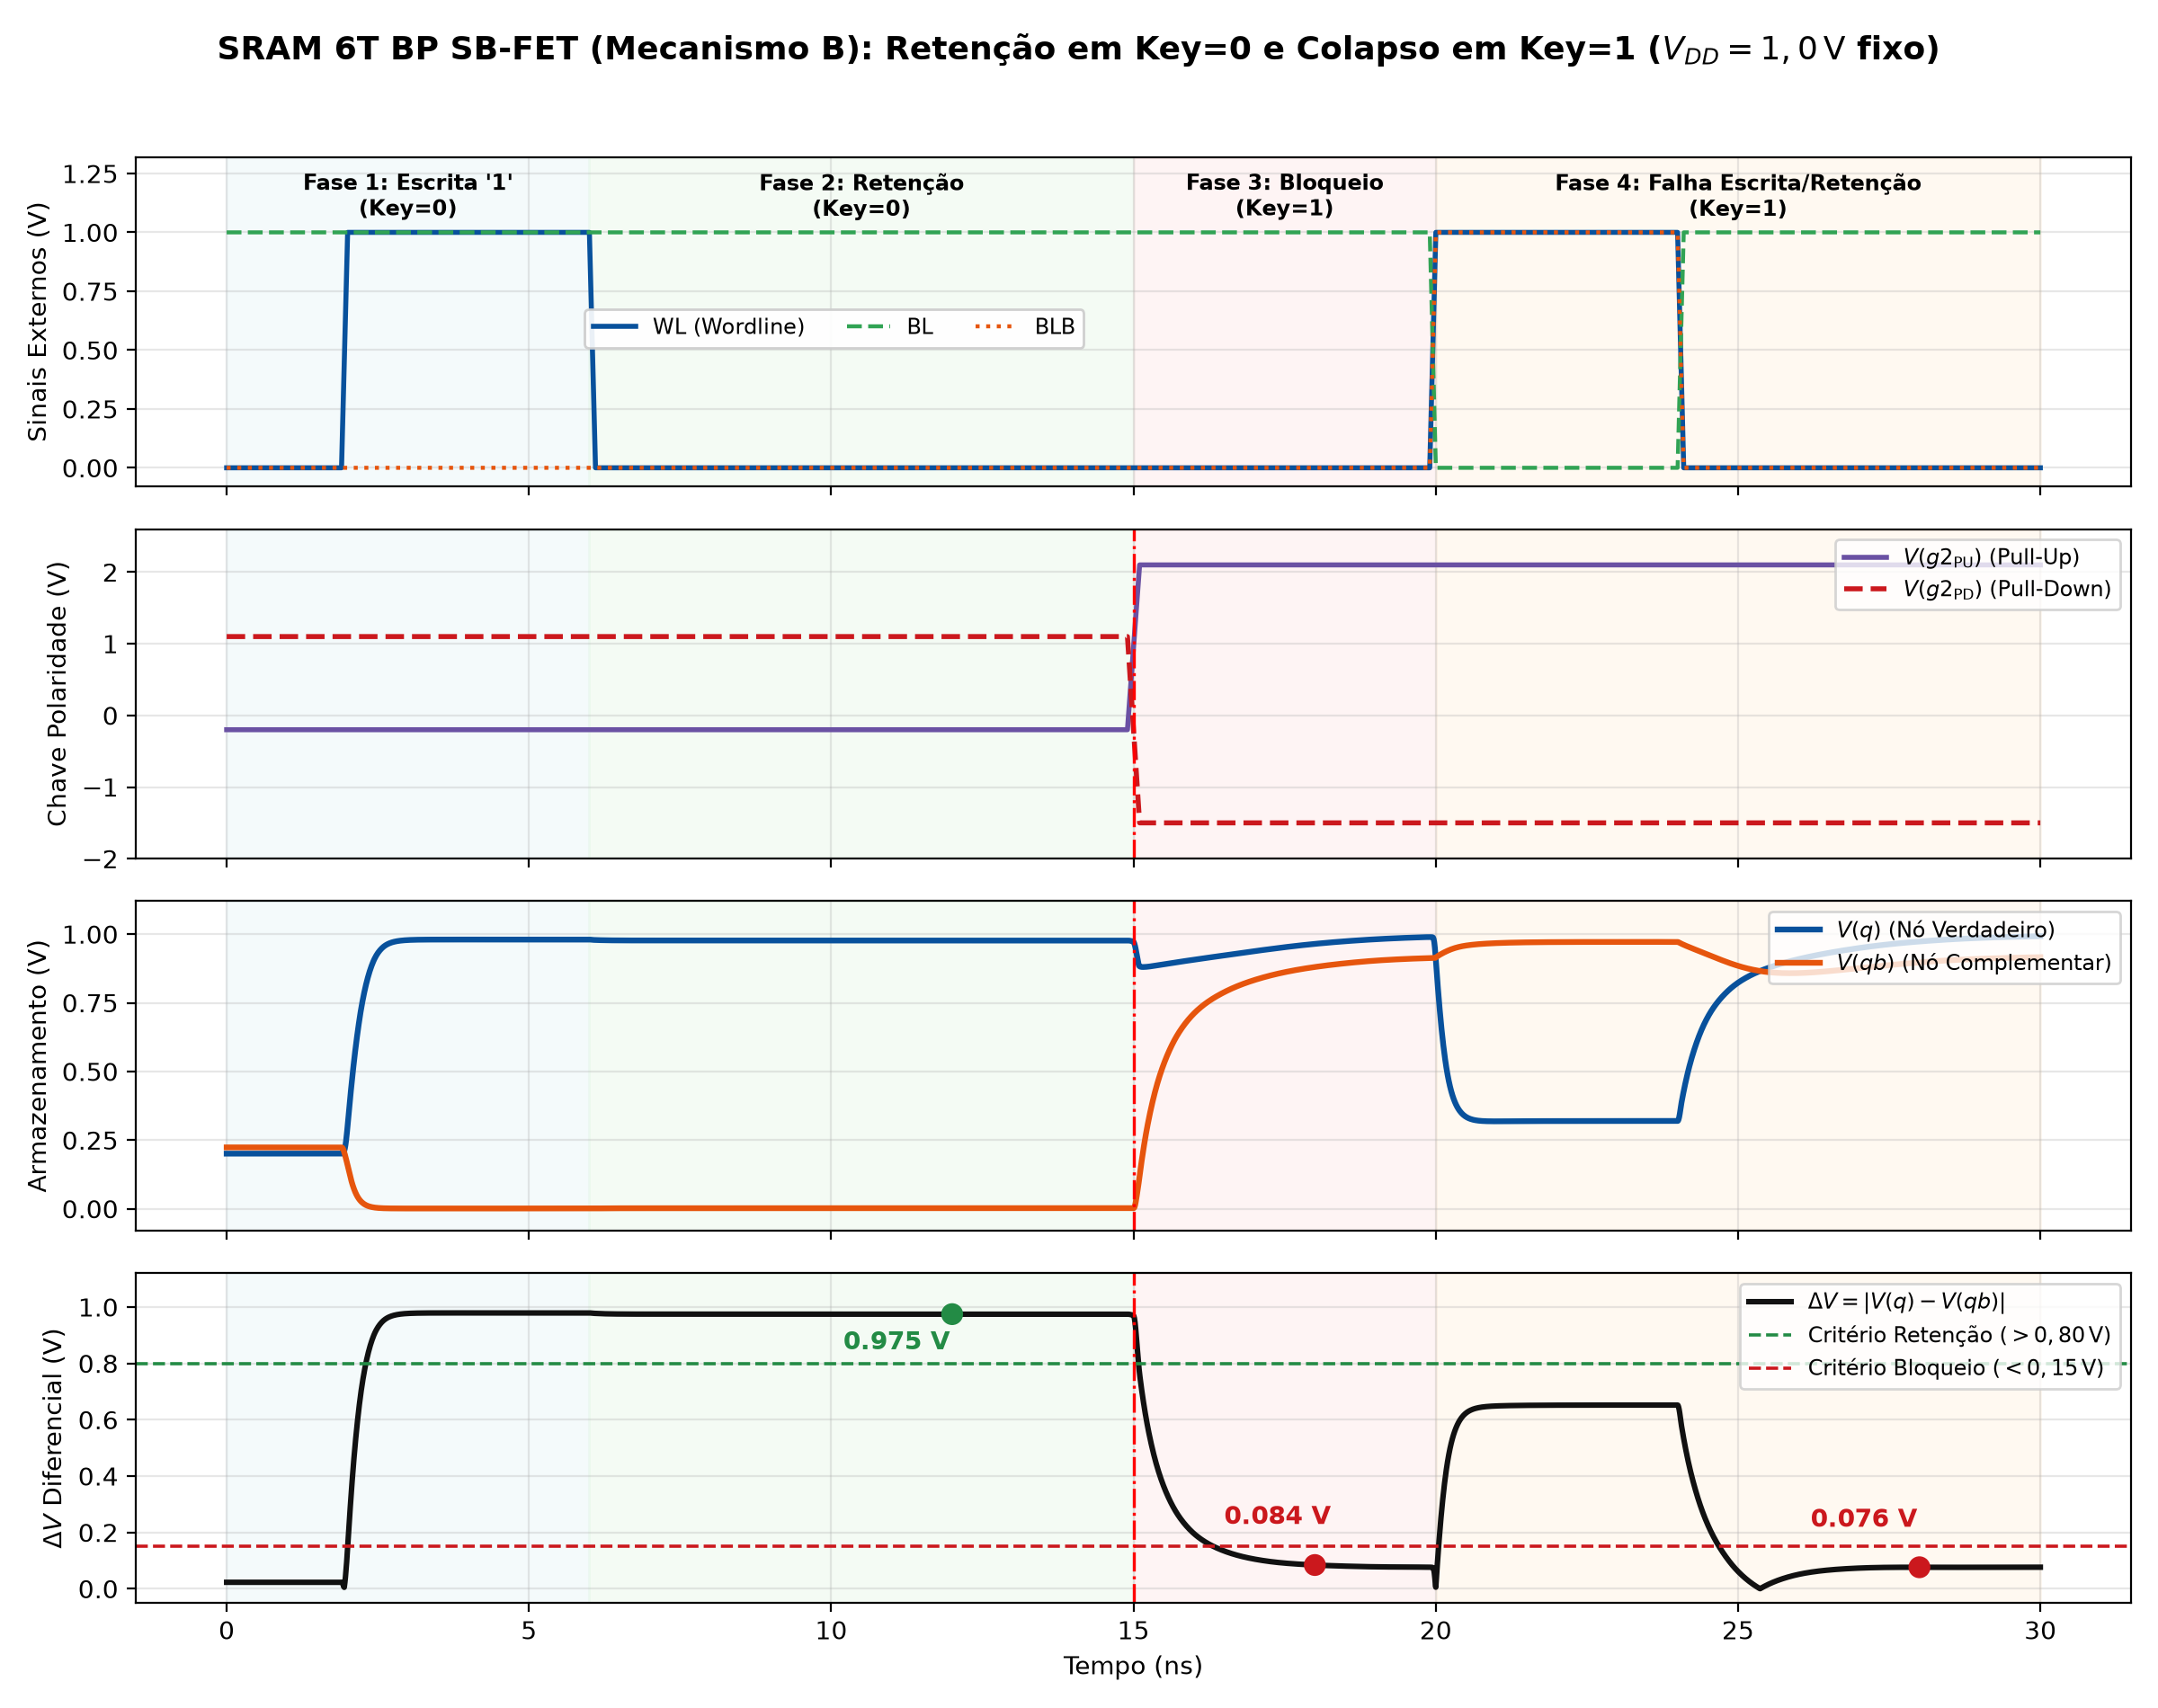
\includegraphics[width=0.92\textwidth]{m04_sram_transiente_30ns.png}
\caption{Simula\c{c}\~{a}o transiente de $30\ \text{ns}$ da SRAM 6T em quatro fases: escrita e reten\c{c}\~{a}o segura sob $\text{Key}=0$ ($0\text{--}15\ \text{ns}$) seguidas de auto-destrui\c{c}\~{a}o do bit e falha de reescrita sob $\text{Key}=1$ ($15\text{--}30\ \text{ns}$).}
\label{fig:m04_tran}
\end{figure}

\begin{figure}[htbp]
\centering
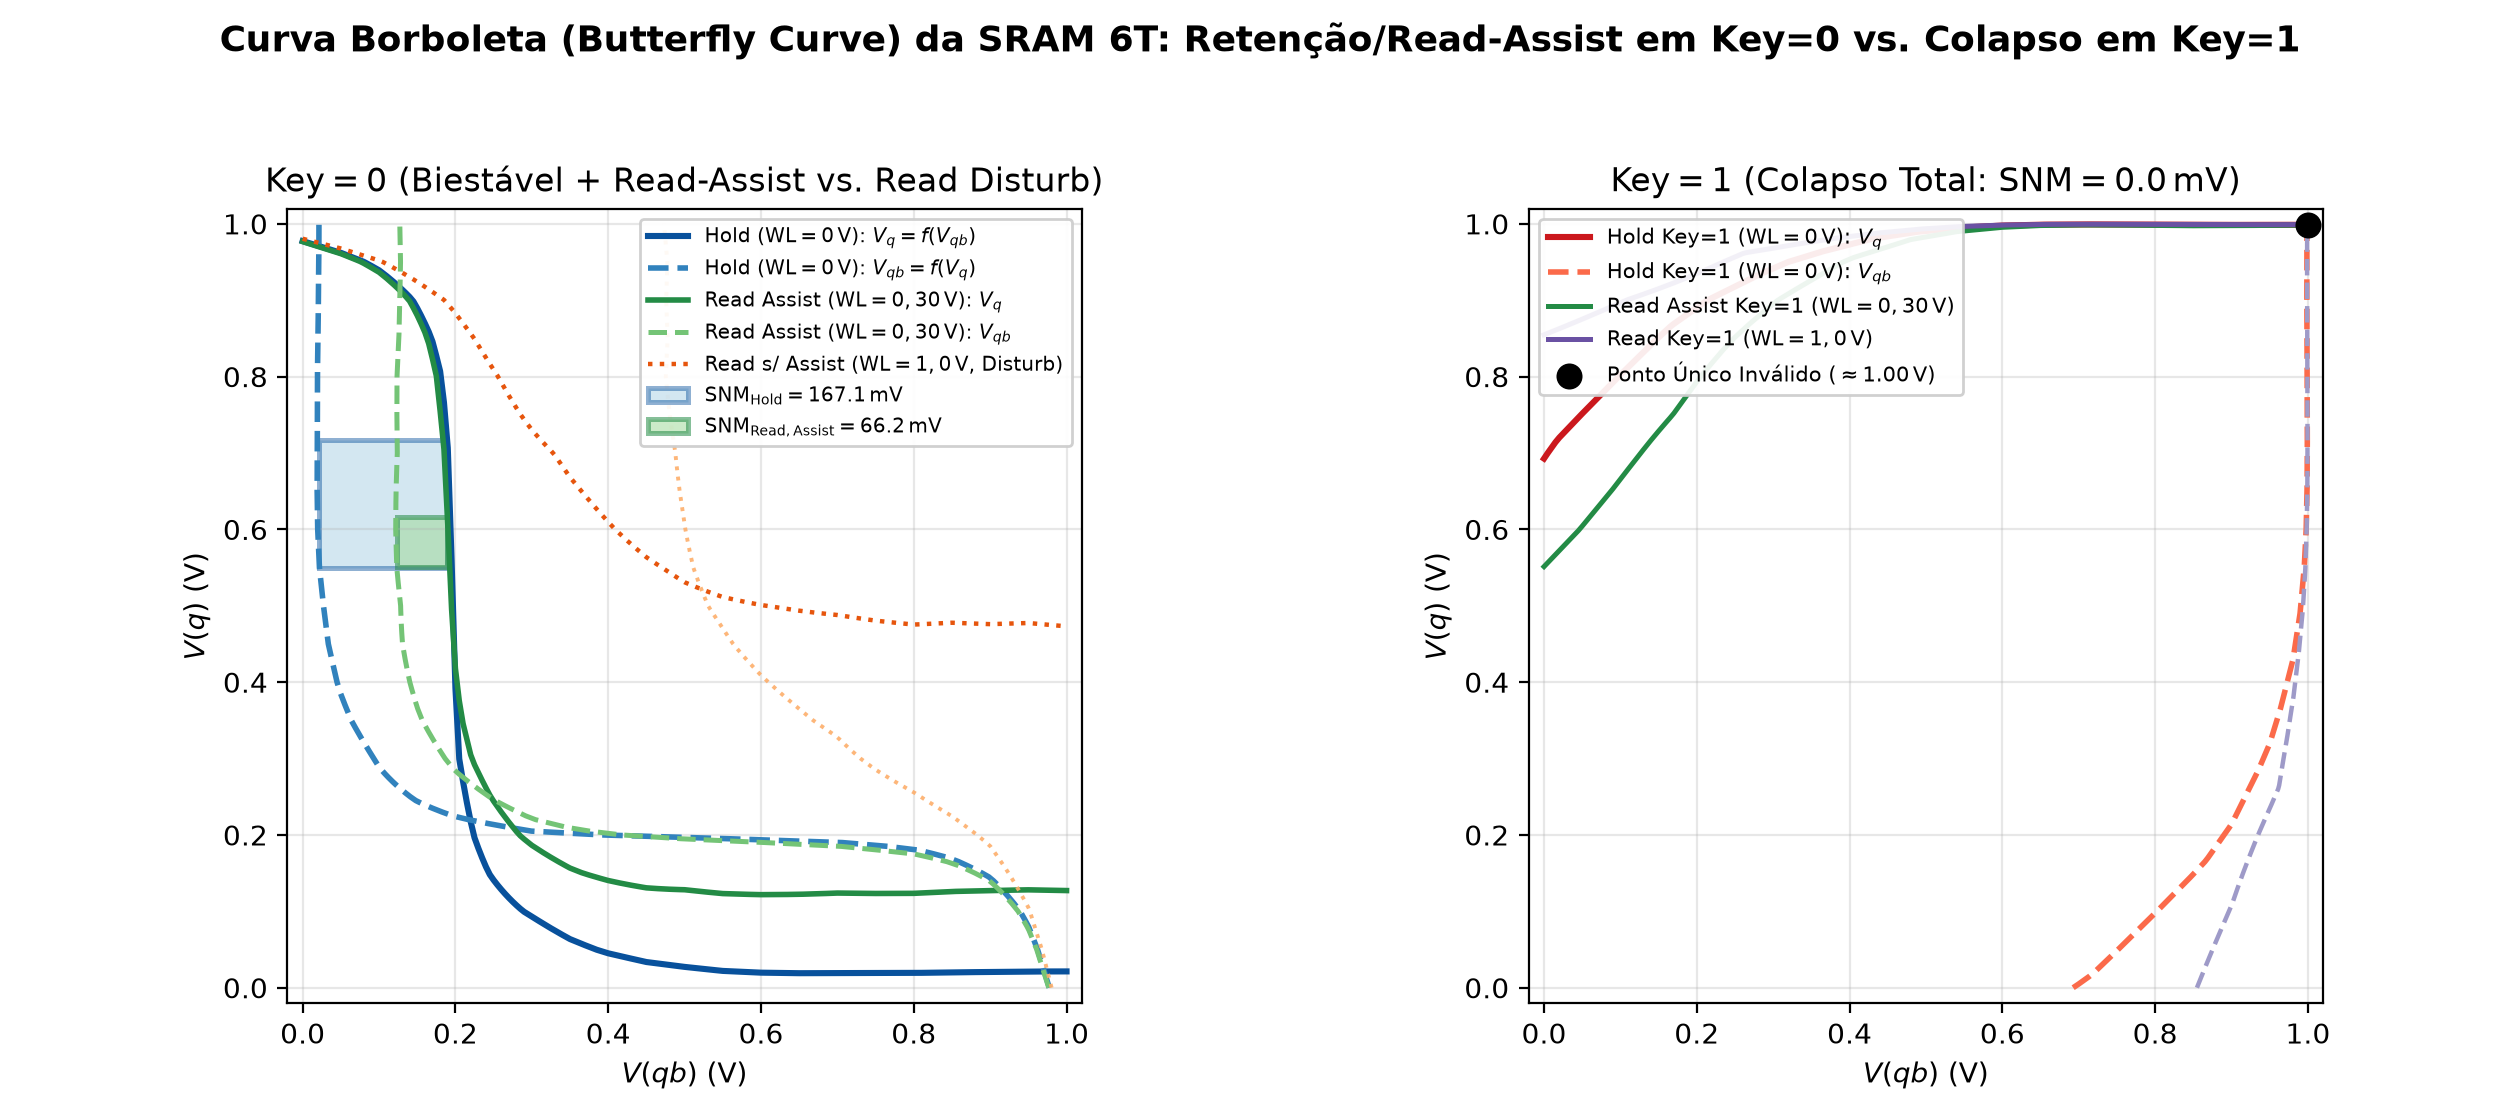
\includegraphics[width=0.92\textwidth]{m04_sram_curva_borboleta_snm.png}
\caption{Curvas borboleta e quadrados m\'{a}ximos inscritos de SNM da SRAM 6T para $\text{Key}=0$ (Hold, Read-Assist e Read sem assist\^{e}ncia com \textit{Read Disturb}) e $\text{Key}=1$ (colapso total para linha monost\'{a}vel).}
\label{fig:m04_snm}
\end{figure}

Dois achados f\'{i}sicos relevantes emergiram da an\'{a}lise das curvas borboleta (Figura~\ref{fig:m04_snm}). Primeiramente, verificou-se com o modelo 4D \texttt{v2} que a polariza\c{c}\~{a}o inicialmente proposta em $V_{g2,\mathrm{PU}} = -0{,}5\ \text{V}$ ($V_{g2,s} = -1{,}5\ \text{V}$) reduz a corrente \textit{p-FET} de $1{,}79$ para $0{,}37\ \mu\text{A}$ (em $V_{gp}=-1{,}0\ \text{V}$) por deslocamento de $V_{fb}$, rebaixando $\mathrm{SNM}_{\mathrm{Hold}}$ para $49{,}4\ \text{mV}$; o ajuste de sintonia para $V_{g2,\mathrm{PU}} = -0{,}2\ \text{V}$ ($V_{g2,s} = -1{,}2\ \text{V}$) restaurou integralmente a simetria sem alterar as larguras $W$, atingindo $\mathrm{SNM}_{\mathrm{Hold}} = 167{,}12\ \text{mV}$. Em segundo lugar, diagnosticou-se o fen\^{o}meno de \textit{Read Disturb} na leitura sem assist\^{e}ncia ($\mathrm{WL}=1{,}0\ \text{V}$, $\mathrm{SNM}=0{,}00\ \text{mV}$), o qual foi mitigado por \textit{Wordline Underdrive Read-Assist} em $\mathrm{WL}=0{,}30\ \text{V}$, recuperando $\mathrm{SNM}_{\mathrm{Read,Assist}} = 66{,}23\ \text{mV}$ enquanto todas as condi\c{c}\~{o}es sob $\text{Key}=1$ mantiveram $\mathrm{SNM}=0{,}00\ \text{mV}$.

\subsection{Somador Completo Polim\'{o}rfico Criptogr\'{a}fico (28 Transistores)}\label{sec:res_fa}

No Somador Completo polim\'{o}rfico de 28 transistores (M\'{o}dulo \texttt{05}), a chave autorizada $K_1 K_0 = 00$ produziu exatid\~{a}o de $100{,}00\%$ nos oito mintermos ($000 \to 111$, Figura~\ref{fig:m05_wave}), sustentando excurs\~{a}o superior a $94\%$ na sa\'{i}da \texttt{Sum} (dom\'{i}nio $1{,}5\ \text{V}$: \texttt{'0'} $\le 0{,}0012\ \text{V}$, \texttt{'1'} $\ge 1{,}4129\ \text{V}$) e superior a $92\%$ na sa\'{i}da \texttt{Cout} (dom\'{i}nio $0{,}8\ \text{V}$: \texttt{'0'} $\le 0{,}0124\ \text{V}$, \texttt{'1'} $\ge 0{,}7526\ \text{V}$) ap\'{o}s tr\^{e}s est\'{a}gios l\'{o}gicos cascateados.

\begin{table}[htbp]
\centering
\caption{Corrup\c{c}\~{a}o funcional e Dist\^{a}ncia de Hamming (HD) por chave criptogr\'{a}fica $(K_1, K_0)$ no Full Adder 28T.}
\label{tab:fa_hamming}
\resizebox{\textwidth}{!}{%
\begin{tabular}{c l c c c c c c}
\toprule
\textbf{Chave} $K_1K_0$ & \textbf{Configura\c{c}\~{a}o} (\texttt{XXOR1} + \texttt{Cout}) & \textbf{Erros} \texttt{Sum} & \textbf{HD} \texttt{Sum} & \textbf{Erros} \texttt{Cout} & \textbf{HD} \texttt{Cout} & \textbf{HD Total} (/16) & \textbf{Acur\'{a}cia} \\
\midrule
\texttt{00} (Correta) & \texttt{XOR} + \texttt{NAND}  & $0/8$ & $0{,}0\%$   & $0/8$ & $0{,}0\%$  & $0\ (0{,}00\%)$   & $100{,}00\%$ \\
\texttt{01} (Errada)  & \texttt{XNOR} + \texttt{NAND} & $8/8$ & $100{,}0\%$ & $3/8$ & $37{,}5\%$ & $11\ (68{,}75\%)$ & $31{,}25\%$  \\
\texttt{10} (Errada)  & \texttt{XOR} + \texttt{NOR}   & $0/8$ & $0{,}0\%$   & $3/8$ & $37{,}5\%$ & $3\ (18{,}75\%)$  & $81{,}25\%$  \\
\texttt{11} (Errada)  & \texttt{XNOR} + \texttt{NOR}  & $8/8$ & $100{,}0\%$ & $0/8$ & $0{,}0\%$  & $8\ (50{,}00\%)$  & $50{,}00\%$  \\
\bottomrule
\end{tabular}}
\end{table}

Conforme a Tabela~\ref{tab:fa_hamming} e a Figura~\ref{fig:m05_hd}, todas as chaves incorretas corrompem a opera\c{c}\~{a}o aritm\'{e}tica sem necessidade de transistores adicionais dedicados a bloqueio. Em $K_1K_0 = 01$, a invers\~{a}o do n\'{o} $P \to \overline{P}$ propaga-se tanto para \texttt{Sum} ($100{,}0\%$) quanto para \texttt{Cout} ($37{,}5\%$), resultando em $\mathrm{HD}_{\mathrm{Total}} = 68{,}75\%$. Em $K_1K_0 = 11$, manifesta-se uma propriedade alg\'{e}brica de dualidade de De Morgan: ao converter simultaneamente \texttt{XXOR1} em \texttt{XNOR} ($\overline{P}$) e \texttt{XG1}--\texttt{XG3} em \texttt{NOR}, obt\'{e}m-se $\overline{\overline{A+B} + \overline{\overline{P}+C_{\mathrm{in}}}} = (A+B)\cdot(\overline{P}+C_{\mathrm{in}}) = A\cdot B + C_{\mathrm{in}}\cdot(A\oplus B)$, restaurando integralmente \texttt{Cout} enquanto \texttt{Sum} permanece $100{,}0\%$ invertida ($\mathrm{HD}_{\mathrm{Total}} = 50{,}00\%$).

\begin{figure}[htbp]
\centering
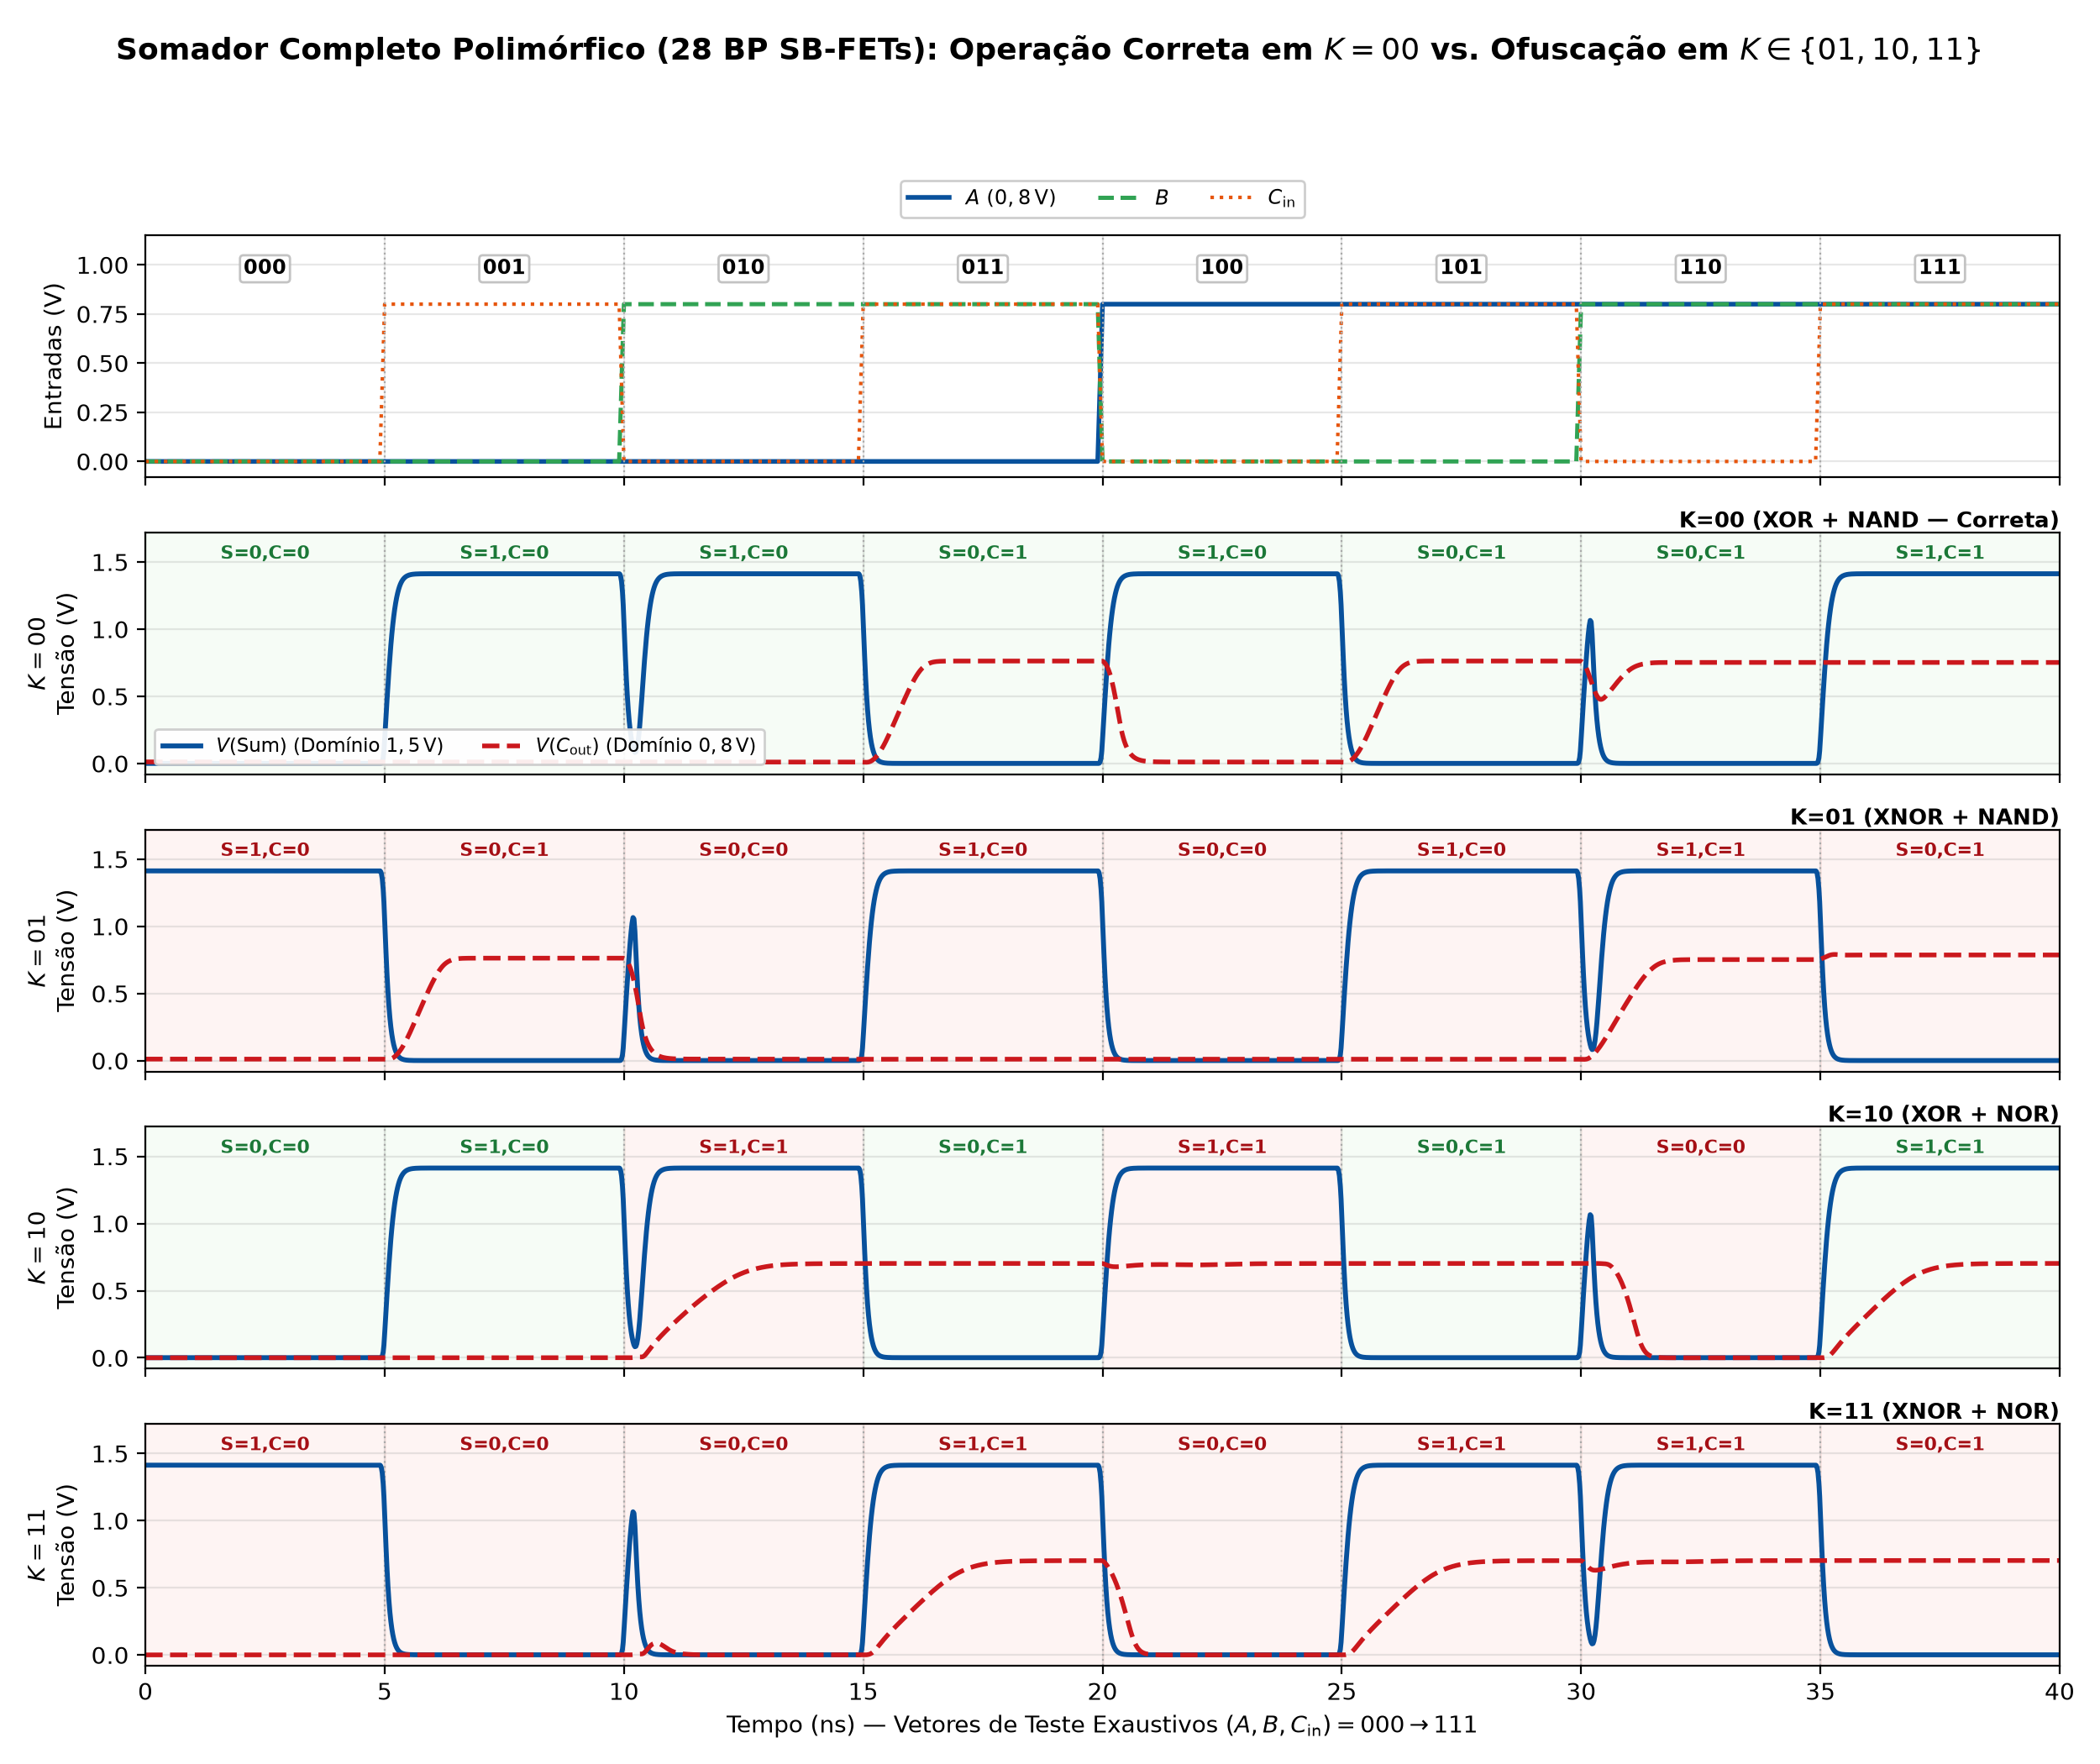
\includegraphics[width=0.92\textwidth]{m05_full_adder_waveforms.png}
\caption{Formas de onda transientes ($40\ \text{ns}$, mintermos \texttt{000} a \texttt{111}) do Somador Completo polim\'{o}rfico de 28 transistores nas quatro chaves $K_1K_0$.}
\label{fig:m05_wave}
\end{figure}

\begin{figure}[htbp]
\centering
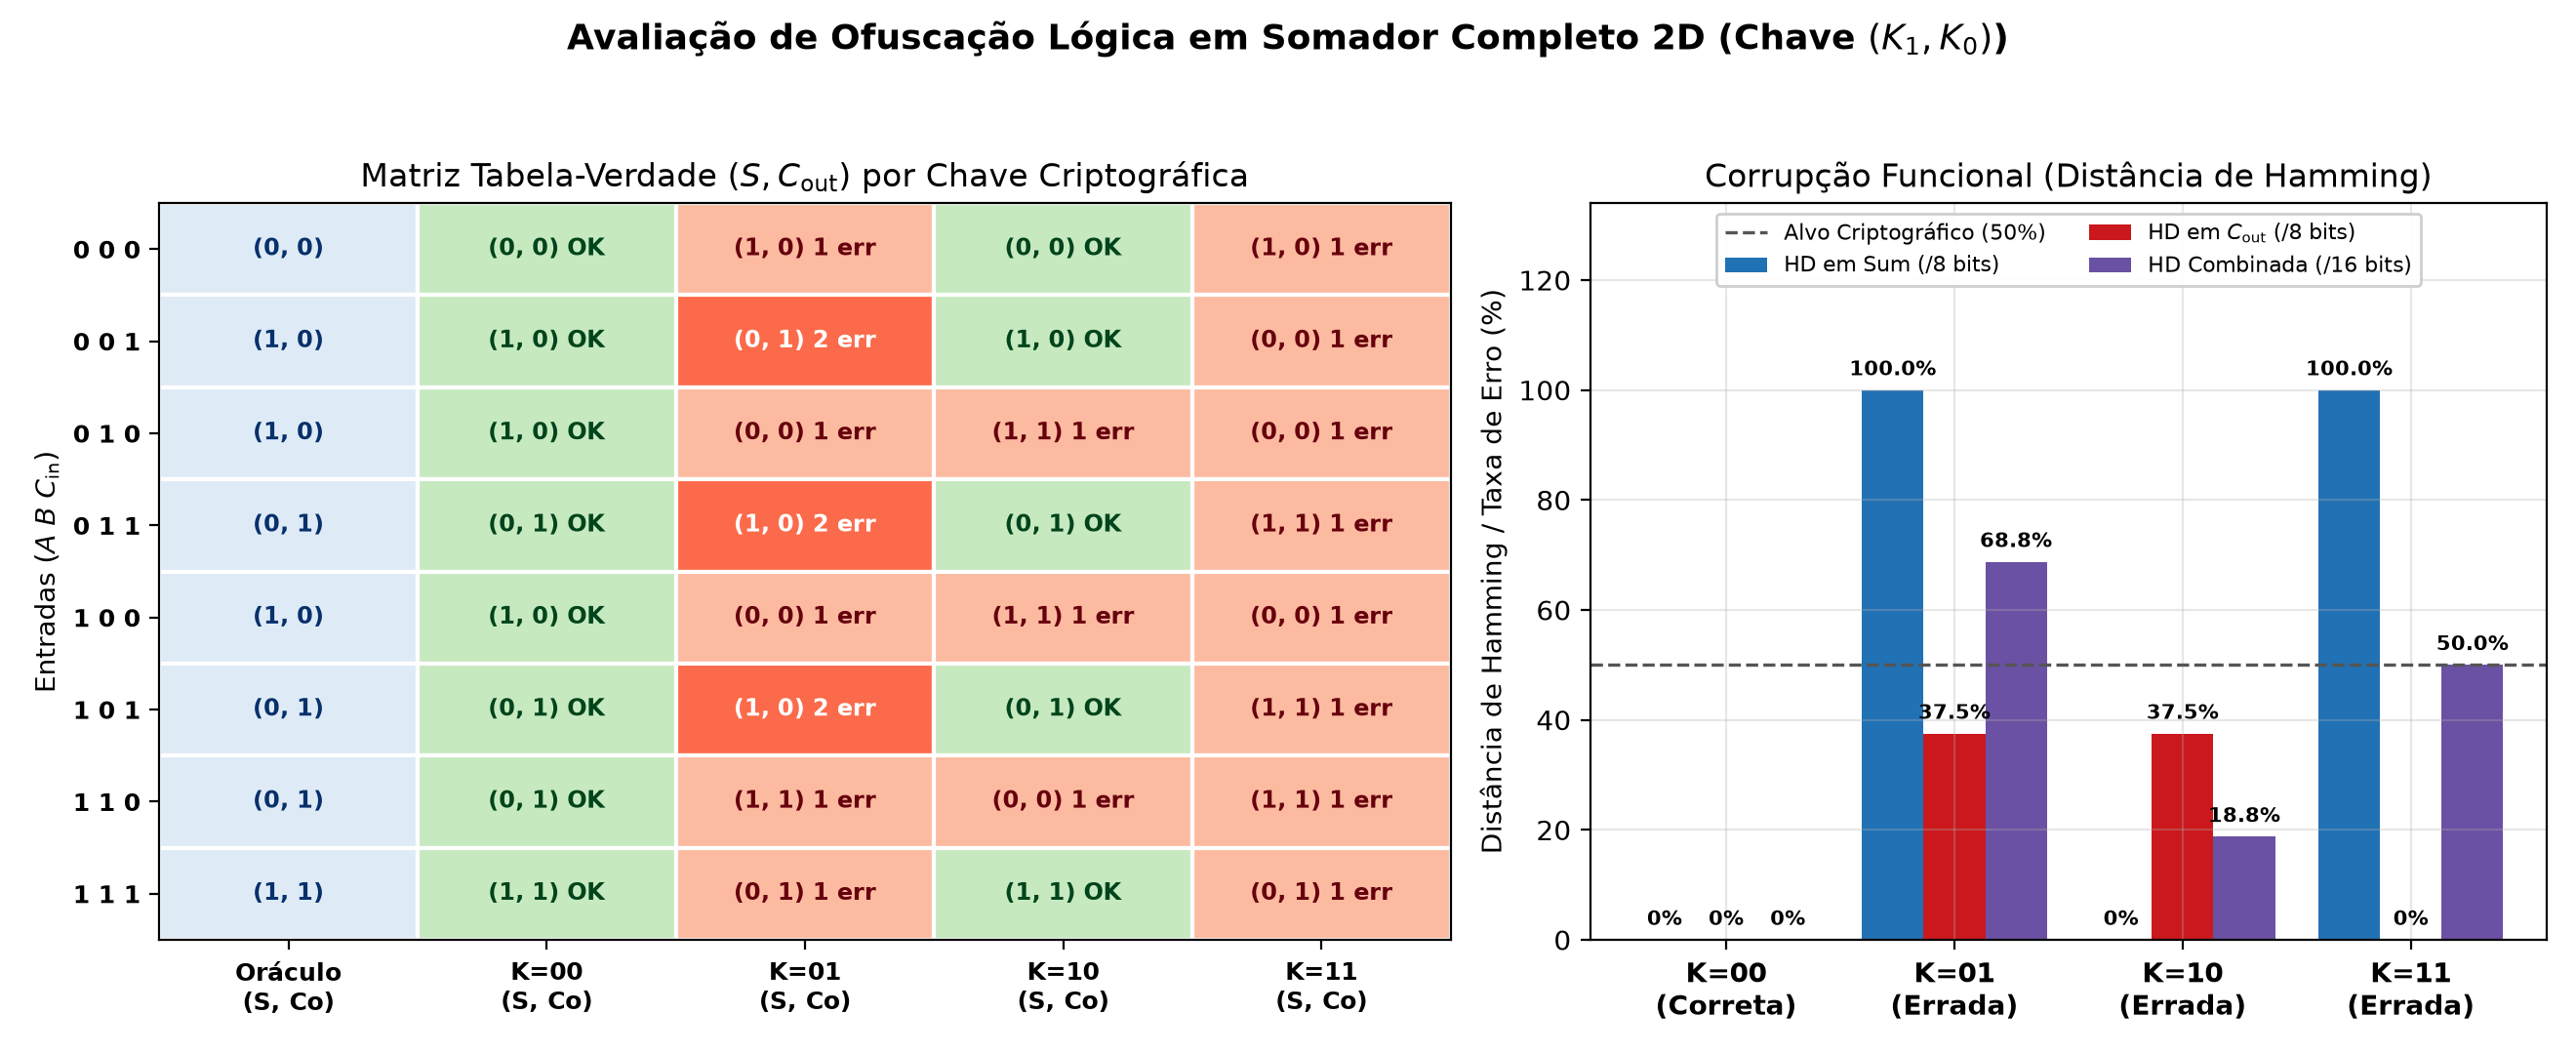
\includegraphics[width=0.92\textwidth]{m05_matriz_tabelas_verdade_hamming.png}
\caption{Matriz de tabelas-verdade e Dist\^{a}ncia de Hamming (HD) do Somador Completo polim\'{o}rfico para as chaves \texttt{00}, \texttt{01}, \texttt{10} e \texttt{11}.}
\label{fig:m05_hd}
\end{figure}

\subsection{Fronteira Operacional sob Tens\~{o}es N\~{a}o Padronizadas}\label{sec:res_fronteira}

A varredura dos 292 pontos dentro do dom\'{i}nio experimentalmente medido das tabelas LUT (M\'{o}dulo \texttt{06}) demonstrou que o deslocamento das tens\~{o}es de alimenta\c{c}\~{a}o, entrada e polaridade pode conduzir aos tr\^{e}s regimes previstos: manuten\c{c}\~{a}o da fun\c{c}\~{a}o nominal (\texttt{CORRETA}), transmuta\c{c}\~{a}o para outra fun\c{c}\~{a}o booleana digital (\texttt{OUTRA\_FUNCAO}) ou colapso em estados anal\'{o}gicos indefinidos (\texttt{INDEFINIDO\_ANALOGICO}), conforme sumarizado na Tabela~\ref{tab:fronteira_resumo}.

\begin{table}[htbp]
\centering
\caption{Distribui\c{c}\~{a}o dos 292 pontos simulados sob tens\~{o}es n\~{a}o padronizadas no dom\'{i}nio das LUTs.}
\label{tab:fronteira_resumo}
\resizebox{\textwidth}{!}{%
\begin{tabular}{l c c c c l}
\toprule
\textbf{Subexperimento} & \textbf{Pontos} & \texttt{CORRETA} & \texttt{OUTRA\_FUNCAO} & \texttt{INDEFINIDO} & \textbf{Fun\c{c}\~{o}es Equivalentes Observadas} \\
\midrule
\texttt{NAND}/\texttt{NOR} ($V_{DD}\times$ Pol.) & $70$  & $29$ & $35$ & $6$  & \texttt{NAND} ($13$), \texttt{NOR} ($17$), \texttt{CONST\_0} ($34$), \texttt{X} ($6$) \\
\texttt{NAND}/\texttt{NOR} ($V_{g2,n}\times V_{g2,p}$) & $72$  & $60$ & $0$  & $12$ & \texttt{NAND} ($27$), \texttt{NOR} ($33$), \texttt{X} ($12$) \\
\texttt{XOR}/\texttt{XNOR} ($V_{DD}\times V_{\mathrm{in}}$) & $100$ & $44$ & $46$ & $10$ & \texttt{XOR} ($22$), \texttt{XNOR} ($22$), \texttt{CONST\_0} ($38$), \texttt{CONST\_1} ($8$), \texttt{X} ($10$) \\
\texttt{XOR}/\texttt{XNOR} ($V_{g,\mathrm{top}}=0\ \text{V}$) & $50$  & $44$ & $6$  & $0$  & \texttt{XOR} ($22$), \texttt{XNOR} ($22$), \texttt{CONST\_1} ($6$) \\
\bottomrule
\end{tabular}}
\end{table}

Na fam\'{i}lia \texttt{NAND}/\texttt{NOR} (Figuras~\ref{fig:m06_nn_vdd} e \ref{fig:m06_nn_asym}), observou-se um evento cr\'{i}tico de \textbf{convers\~{a}o espont\^{a}nea \texttt{NAND} $\to$ \texttt{NOR} sem altera\c{c}\~{a}o da chave}: em $V_{DD} = 0{,}65\ \text{V}$ sob sub-polariza\c{c}\~{a}o moderada ($+0{,}4/-1{,}1\ \text{V}$), a porta configurada como \texttt{NAND} ($\text{Key}=0$) produziu o padr\~{a}o l\'{o}gico \texttt{[1000]} ($V_{00}=0{,}5412\ \text{V}$, $V_{01}=0{,}1073\ \text{V}$, $V_{10}=0{,}1410\ \text{V}$, $V_{11}=0{,}0206\ \text{V}$), id\^{e}ntico \`{a} tabela-verdade da sua fun\c{c}\~{a}o dual \texttt{NOR}. Fisicamente, nos vetores \texttt{01} e \texttt{10}, apenas um \textit{p-FET} enfraquecido tenta elevar a sa\'{i}da enquanto a rede s\'{e}rie \textit{n-FET} em $+0{,}4\ \text{V}$ sustenta fuga suficiente para descarregar o n\'{o}, vencendo o \textit{pull-up} somente quando os dois \textit{p-FETs} conduzem em paralelo (\texttt{00}). Para $V_{DD} \le 0{,}50\ \text{V}$, $34$ dos $70$ pontos degeneraram em \texttt{CONST\_0} (\texttt{0000}). Na grade de assimetria em $V_{DD}=0{,}80\ \text{V}$, $60$ de $72$ pontos operaram corretamente e $12$ entraram em regime anal\'{o}gico indefinido (\texttt{[1X10]}, \texttt{[10X0]}, \texttt{[111X]}, \texttt{[X000]}), com destaque para a faixa n\~{a}o monot\^{o}nica em $V(g2,s)_p = -1{,}50\ \text{V}$ na \texttt{NAND} (em raz\~{a}o do deslocamento $\Delta V_{fb} \approx -0{,}25\ \text{V}$, $V_{01}$ colapsou para $0{,}163\text{--}0{,}496\ \text{V}$ em quatro das seis colunas \textit{n-FET}), ao passo que $V(g2,s)_p \in \{-1{,}35;\ -1{,}20\}\ \text{V}$ obteve $100\%$ de acerto.

Na fam\'{i}lia \texttt{XOR}/\texttt{XNOR} (Figura~\ref{fig:m06_xor_mapa}), avaliaram-se $150$ pontos ($88$ corretos, $52$ classificados como \texttt{OUTRA\_\allowbreak FUNCAO} e $10$ em estado indefinido \texttt{INDEFINIDO\_\allowbreak ANALOGICO}), revelando travamentos sim\'{e}tricos opostos: para $V_{DD} \in [0{,}60;\ 0{,}80]\ \text{V}$, $38$ casos degeneraram para \texttt{CONST\_0} (\texttt{0000}) por \textit{overdrive} insuficiente do ramo \textit{p-FET}; inversamente, com $V_{DD}$ elevado ($1{,}20\text{--}1{,}50\ \text{V}$) e $V_{\mathrm{in}}$ baixo ($0{,}40\text{--}0{,}60\ \text{V}$), $14$ casos travaram em \texttt{CONST\_1} (\texttt{1111}, $V_{\mathrm{out}} \ge 1{,}4154\ \text{V}$ a $1{,}50\ \text{V}$) acompanhados de elevada corrente est\'{a}tica ($0{,}536\text{--}1{,}222\ \mu\text{A}$). Na fronteira intermedi\'{a}ria ($V_{DD} = 1{,}00\ \text{V}$), a polariza\c{c}\~{a}o nominal ($+0{,}8/-1{,}5\ \text{V}$) entrou em regime indefinido para $V_{\mathrm{in}} \ge 0{,}80\ \text{V}$, enquanto a sub-polariza\c{c}\~{a}o ($+0{,}2/-0{,}9\ \text{V}$) restaurou a opera\c{c}\~{a}o correta com margem normalizada entre $86{,}4\%$ e $88{,}4\%$.

\begin{figure}[htbp]
\centering
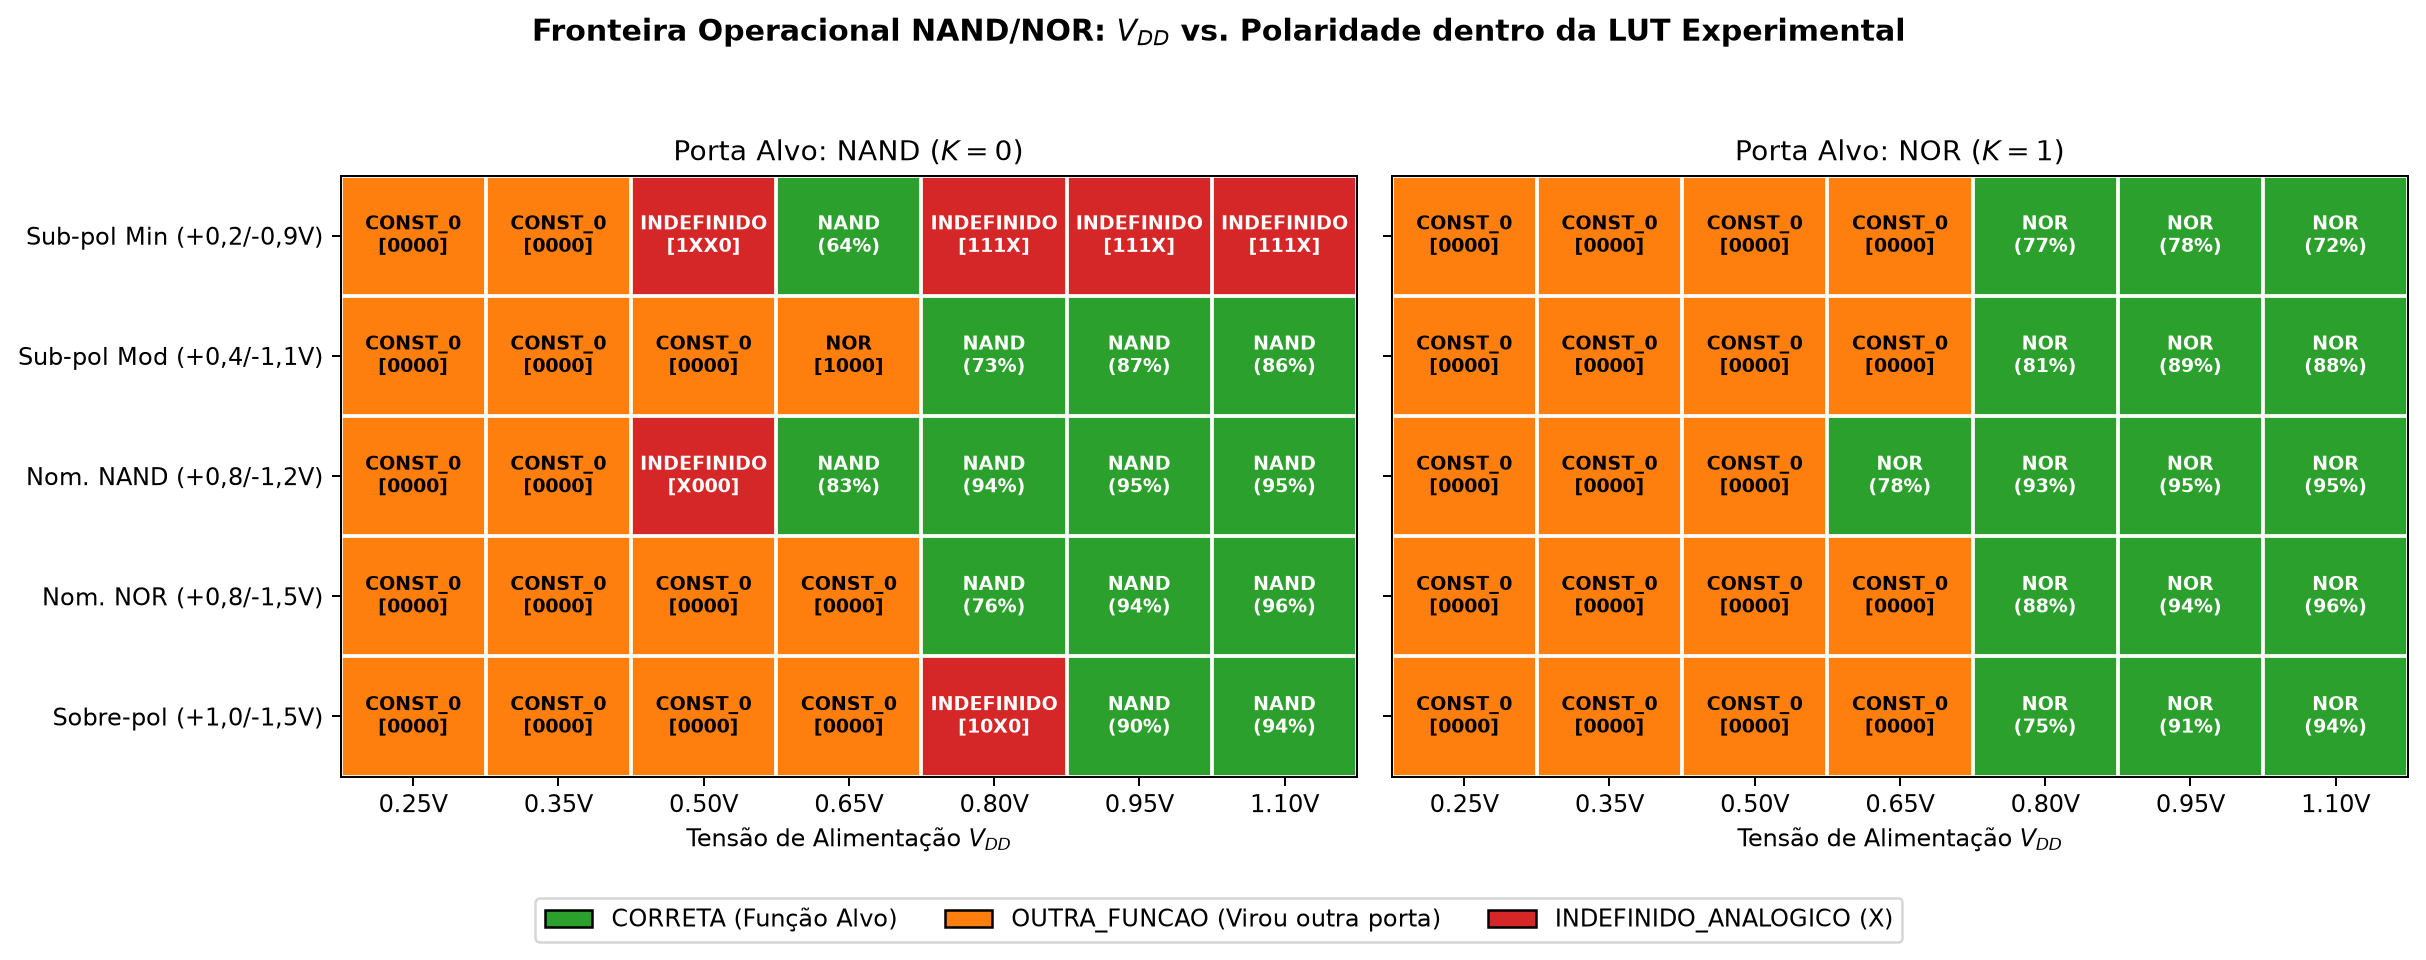
\includegraphics[width=0.92\textwidth]{m06_nand_nor_mapa_vdd_polaridade.png}
\caption{Mapa de fases operacionais ($V_{DD} \times$ polaridade) da porta \texttt{NAND}/\texttt{NOR}, destacando a convers\~{a}o espont\^{a}nea \texttt{NAND} $\to$ \texttt{NOR} em $V_{DD}=0{,}65\ \text{V}$ e o colapso \texttt{CONST\_0} em sub-tens\~{a}o.}
\label{fig:m06_nn_vdd}
\end{figure}

\begin{figure}[htbp]
\centering
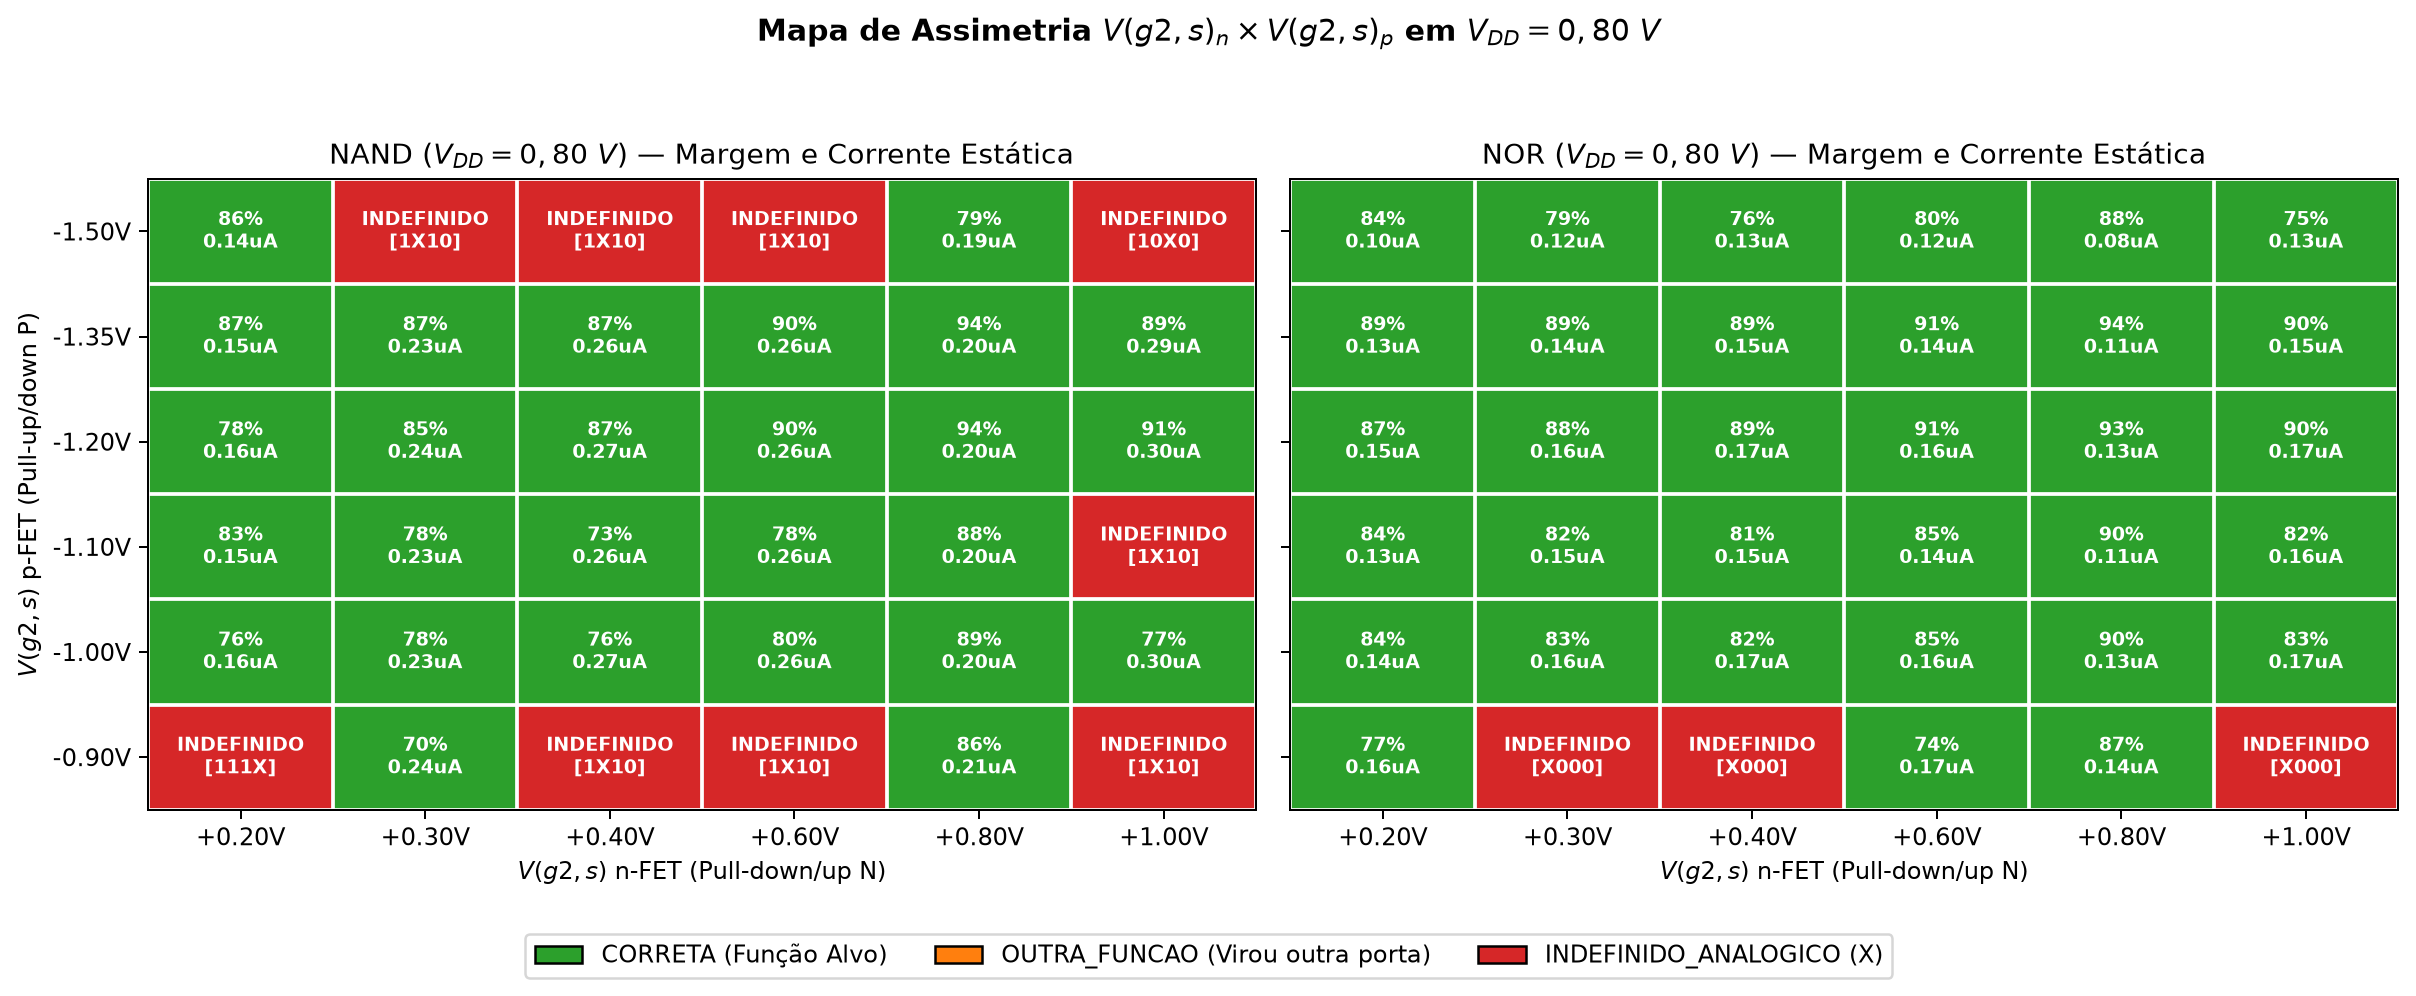
\includegraphics[width=0.92\textwidth]{m06_nand_nor_assimetria_vg2.png}
\caption{Mapa de assimetria $V(g2,s)_n \times V(g2,s)_p$ em $V_{DD}=0{,}80\ \text{V}$ para \texttt{NAND} e \texttt{NOR}, evidenciando a degrada\c{c}\~{a}o n\~{a}o monot\^{o}nica em $V(g2,s)_p = -1{,}50\ \text{V}$.}
\label{fig:m06_nn_asym}
\end{figure}

\begin{figure}[htbp]
\centering
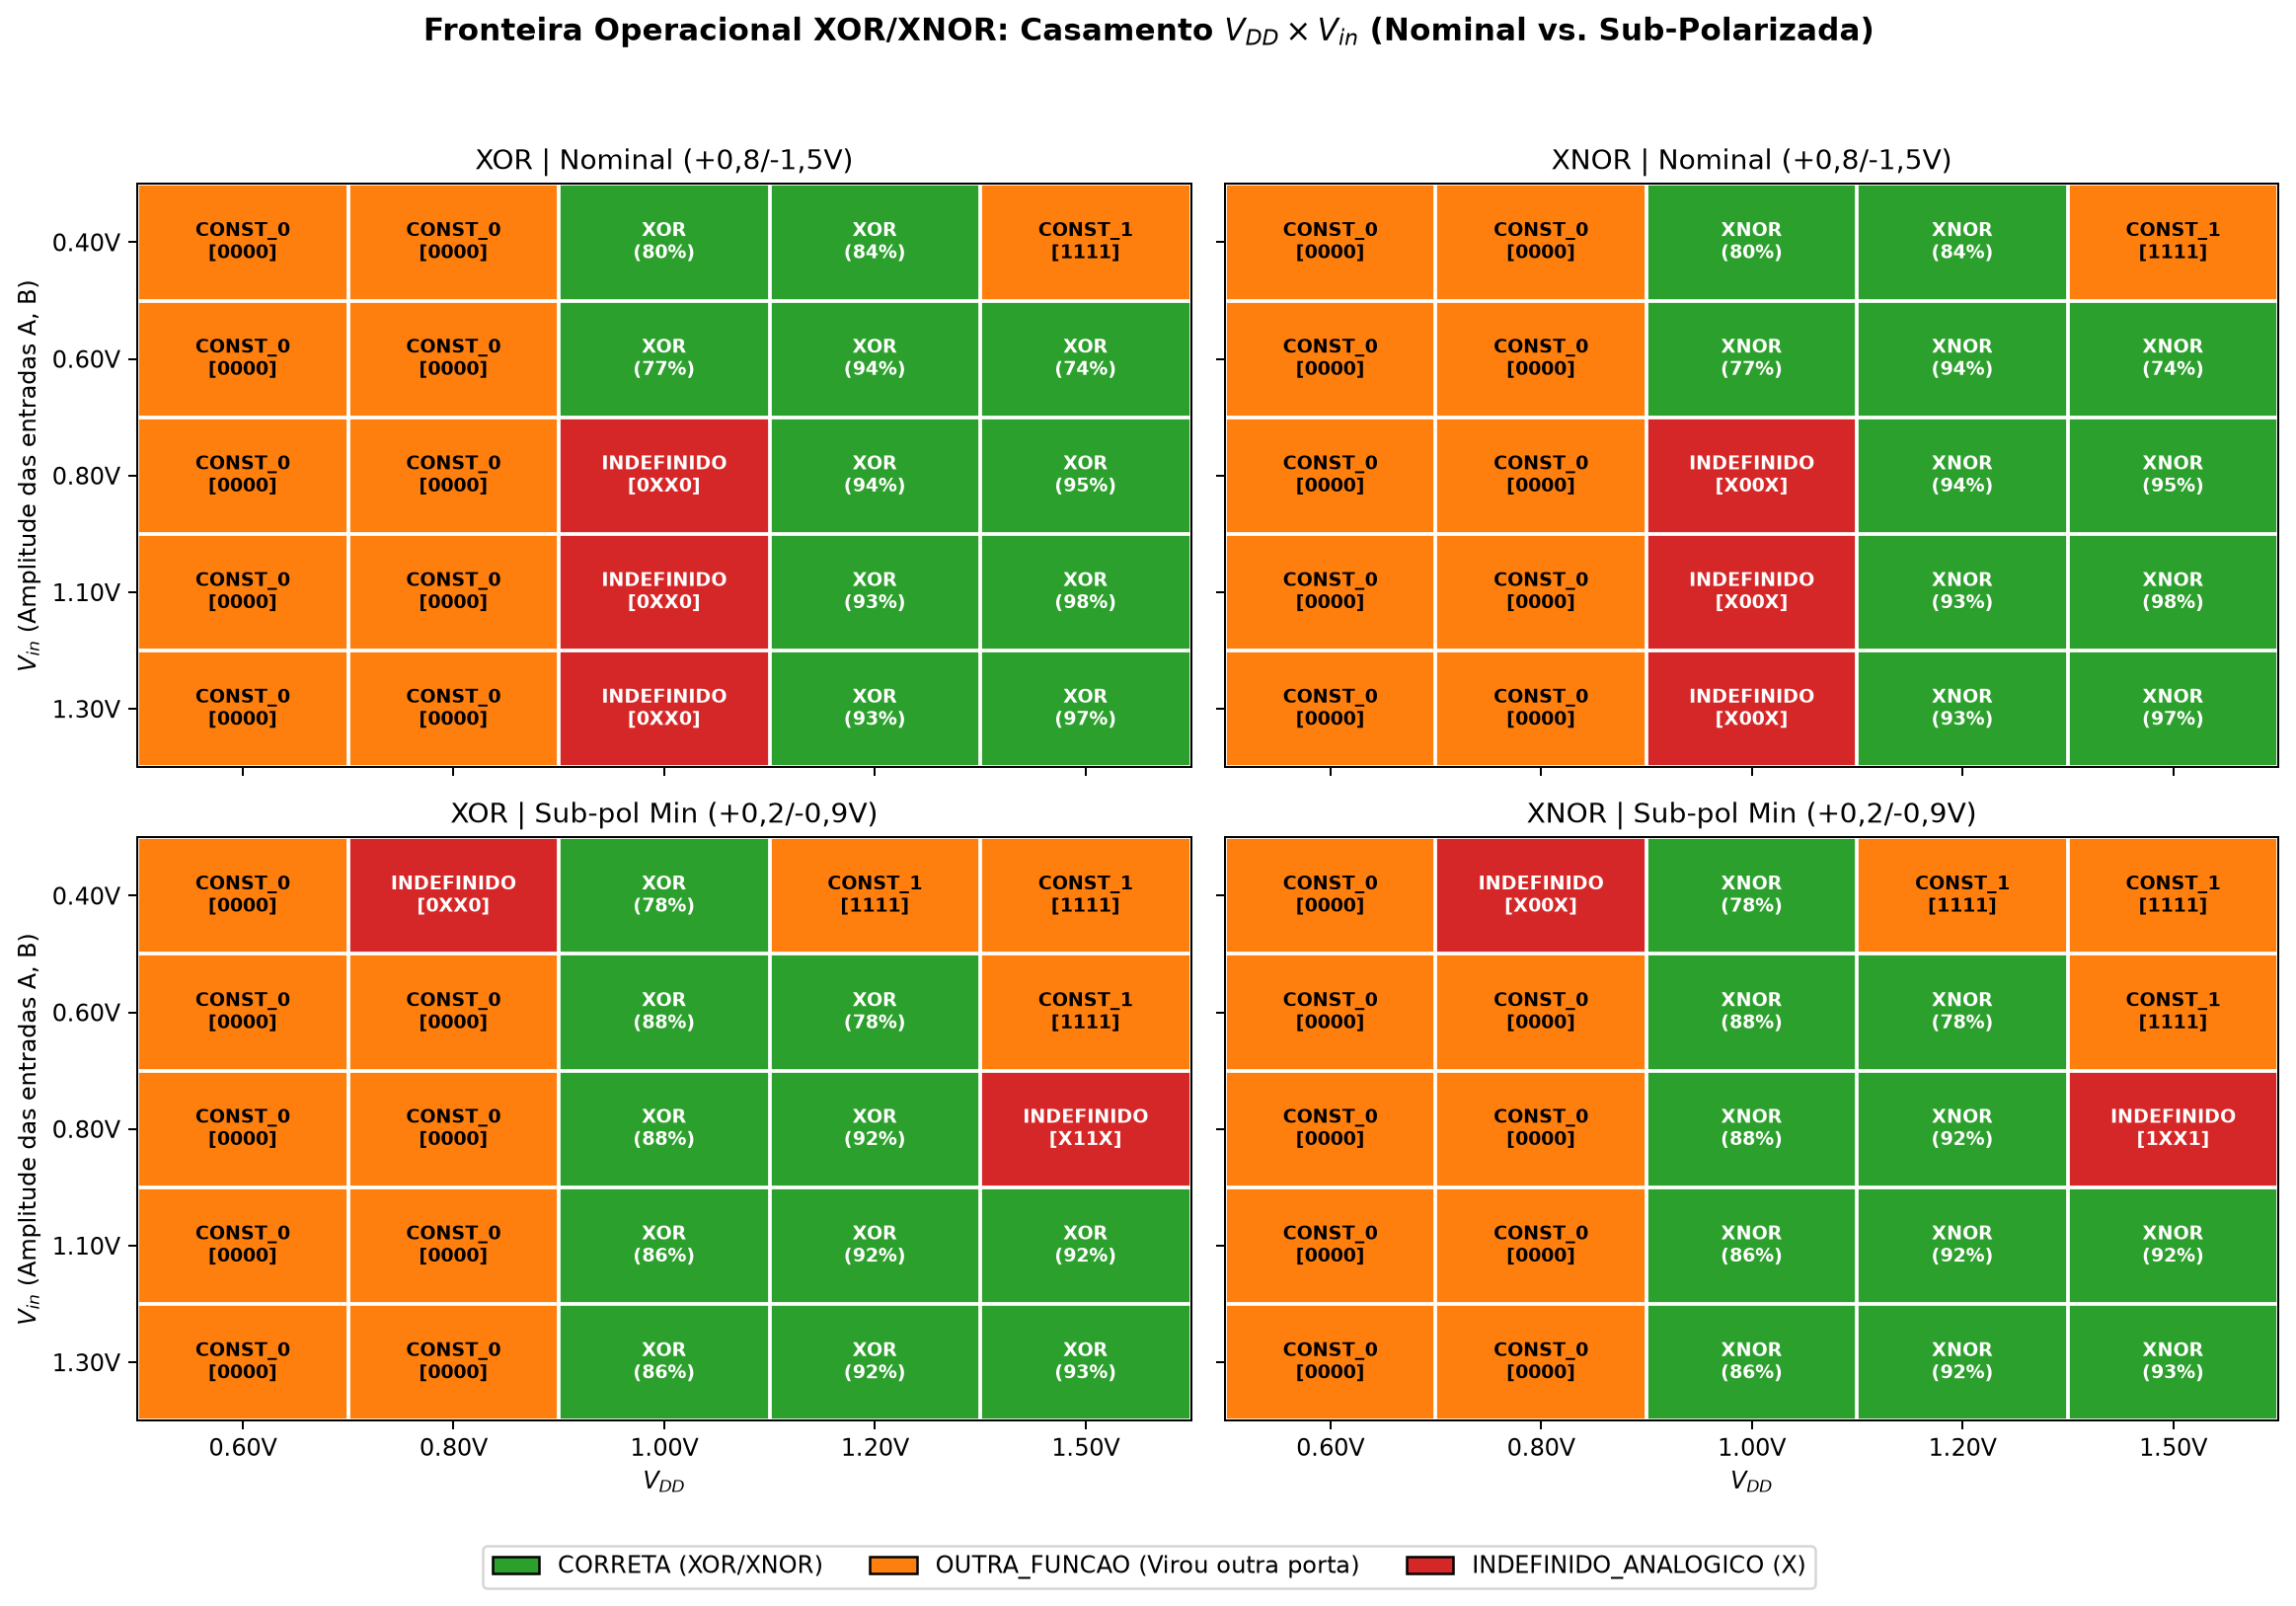
\includegraphics[width=0.92\textwidth]{m06_xor_xnor_mapa_vdd_vin.png}
\caption{Mapa operacional $V_{DD} \times V_{\mathrm{in}}$ da porta \texttt{XOR}/\texttt{XNOR} sob polaridade nominal, sub-polariza\c{c}\~{a}o e porta fixa, expondo as zonas \texttt{CONST\_0}, \texttt{CONST\_1} e indefinida.}
\label{fig:m06_xor_mapa}
\end{figure}

\subsection{Assimetria DPA em Sete Tuplas Polim\'{o}rficas e \textit{Benchmark} do Full Adder}\label{sec:res_tuplas}

No M\'{o}dulo \texttt{07}, todas as $72$ combina\c{c}\~{o}es de entrada e chave avaliadas sobre as sete tuplas atingiram $100{,}0\%$ de corretude l\'{o}gica ($V_{1,\min} \ge 0{,}6792\ \text{V}$ em $0{,}8\ \text{V}$ e $\ge 1{,}3767\ \text{V}$ em $1{,}5\ \text{V}$; $V_{0,\max} \le 0{,}0128\ \text{V}$). A Tabela~\ref{tab:tuplas_dpa} consolida integralmente as m\'{e}tricas de custo, seguran\c{c}a DPA, desempenho din\^{a}mico e robustez Monte Carlo.

\begin{table}[htbp]
\centering
\caption{M\'{e}tricas consolidadas de custo, assimetria DPA, desempenho e robustez Monte Carlo nas sete tuplas polim\'{o}rficas ($C_{\mathrm{load}} = 0{,}3\ \text{fF}$).}
\label{tab:tuplas_dpa}
\resizebox{\textwidth}{!}{%
\begin{tabular}{l c c c c c c c c c c c c}
\toprule
\textbf{Tupla} & \textbf{N\'{u}c./Tot.} & $\sum W$ ($\mu\text{m}$) & $V_{DD}$ (V) & $I_{\mathrm{pico}}$ M0/M1 ($\mu\text{A}$) & \textbf{DPA Pico} & \textbf{DPA M\'{e}d.} & $t_p$ (ps) & $P_{\mathrm{m\acute{e}d}}$ (nW) & $E_{\mathrm{sw}}$ (fJ) & \textbf{PDP} (aJ) & \textbf{MC} ($N=250$) \\
\midrule
\texttt{(NAND, NOR)}   & 4T / 4T   & $6{,}0$  & $0{,}8$ & $0{,}5643$ / $0{,}2138$ & $163{,}91\%$ & $44{,}62\%$ & $554{,}28$ & $40{,}17$  & $0{,}5022$ & $22{,}27$ & $100{,}00\%$ \\
\texttt{(XOR, XNOR)}   & 4T / 8T   & $4{,}0$  & $1{,}5$ & $1{,}6914$ / $1{,}6914$ & $0{,}00\%$   & $30{,}57\%$ & $151{,}84$ & $102{,}47$ & $1{,}2808$ & $15{,}56$ & $100{,}00\%$ \\
\texttt{(AND, OR)}     & 6T / 6T   & $9{,}0$  & $0{,}8$ & $1{,}7345$ / $1{,}8394$ & $6{,}05\%$   & $30{,}87\%$ & $454{,}27$ & $48{,}04$  & $0{,}6005$ & $21{,}82$ & $100{,}00\%$ \\
\texttt{(NAND, XNOR)}  & 6T / 10T  & $8{,}0$  & $1{,}5$ & $1{,}7050$ / $1{,}3387$ & $27{,}36\%$  & $73{,}87\%$ & $163{,}46$ & $94{,}14$  & $1{,}1768$ & $15{,}39$ & $100{,}00\%$ \\
\texttt{(NOR, XOR)}    & 6T / 10T  & $8{,}0$  & $1{,}5$ & $1{,}7129$ / $1{,}6932$ & $1{,}16\%$   & $29{,}60\%$ & $144{,}87$ & $121{,}49$ & $1{,}5186$ & $17{,}60$ & $100{,}00\%$ \\
\texttt{(AOI21, OAI21)}& 6T / 6T   & $12{,}0$ & $0{,}8$ & $0{,}6810$ / $0{,}4299$ & $58{,}44\%$  & $19{,}22\%$ & $555{,}72$ & $59{,}97$  & $0{,}4498$ & $33{,}33$ & $99{,}55\%$  \\
\texttt{(MAJ3, XOR3)}  & 10T / 18T & $18{,}0$ & $1{,}5$ & $1{,}4360$ / $1{,}4355$ & $0{,}04\%$   & $47{,}08\%$ & $180{,}71$ & $212{,}44$ & $1{,}9119$ & $38{,}39$ & $100{,}00\%$ \\
\bottomrule
\end{tabular}}
\end{table}

Sob o testbench padronizado no \texttt{ngspice-47}, as assinaturas de corrente (Figura~\ref{fig:m07_assinaturas}) e a fronteira de Pareto (Figura~\ref{fig:m07_pareto}) revelam compromissos claros de projeto:
\begin{itemize}
    \item \texttt{(NAND, NOR)} apresenta o menor custo f\'{i}sico ($4\text{T}$, $40{,}17\ \text{nW}$), por\'{e}m sofre elevada exposi\c{c}\~{a}o de pico DPA ($163{,}91\%$) e atraso elevado ($554{,}28\ \text{ps}$) devido \`{a} assimetria entre redes paralela ($W=1{,}0$) e s\'{e}rie ($W=2{,}0$).
    \item \texttt{(XOR, XNOR)} elimina integralmente a assimetria de pico ($0{,}00\%$, $1{,}6914\ \mu\text{A}$ em ambos os modos) mantendo $\mathrm{PDP} = 15{,}56\ \text{aJ}$.
    \item Em \texttt{(AND, OR)}, a adi\c{c}\~{a}o do inversor \texttt{BP\_INV08} ($+2\text{T}$) desacopla a carga da rede polim\'{o}rfica e reduz a assimetria global de pico na alimenta\c{c}\~{a}o para $6{,}05\%$, embora a assimetria espec\'{i}fica das transi\c{c}\~{o}es $1 \to 0$ permane\c{c}a alta ($116{,}90\%$).
    \item Entre as c\'{e}lulas mistas, \texttt{(NOR, XOR)} destaca-se como excelente compromisso para \textit{logic locking} heterog\^{e}neo ($1{,}16\%$ de assimetria de pico e menor atraso m\'{e}dio da su\'{i}te: $144{,}87\ \text{ps}$), enquanto \texttt{(NAND, XNOR)} exibe alta assimetria m\'{e}dia ($73{,}87\%$) pelo desbalanceamento de ocorr\^{e}ncia de \texttt{'1'} na tabela da \texttt{NAND} ($75\%$) frente \`{a} \texttt{XNOR} ($50\%$).
    \item Nas portas de tr\^{e}s entradas, \texttt{(AOI21, OAI21)} alcan\c{c}a a menor assimetria m\'{e}dia ($19{,}22\%$) e menor energia de chaveamento ($0{,}4498\ \text{fJ}$) em $6\text{T}$, com pequena redu\c{c}\~{a}o de taxa de acerto Monte Carlo ($99{,}55\%$, Figura~\ref{fig:m07_mc}) por empilhamento em \texttt{OAI21}; j\'{a} \texttt{(MAJ3, XOR3)} estende o equil\'{i}brio quad-sim\'{e}trico a tr\^{e}s entradas com $0{,}04\%$ de DPA de pico e $100{,}0\%$ de acerto estat\'{i}stico.
\end{itemize}

\begin{figure}[htbp]
\centering
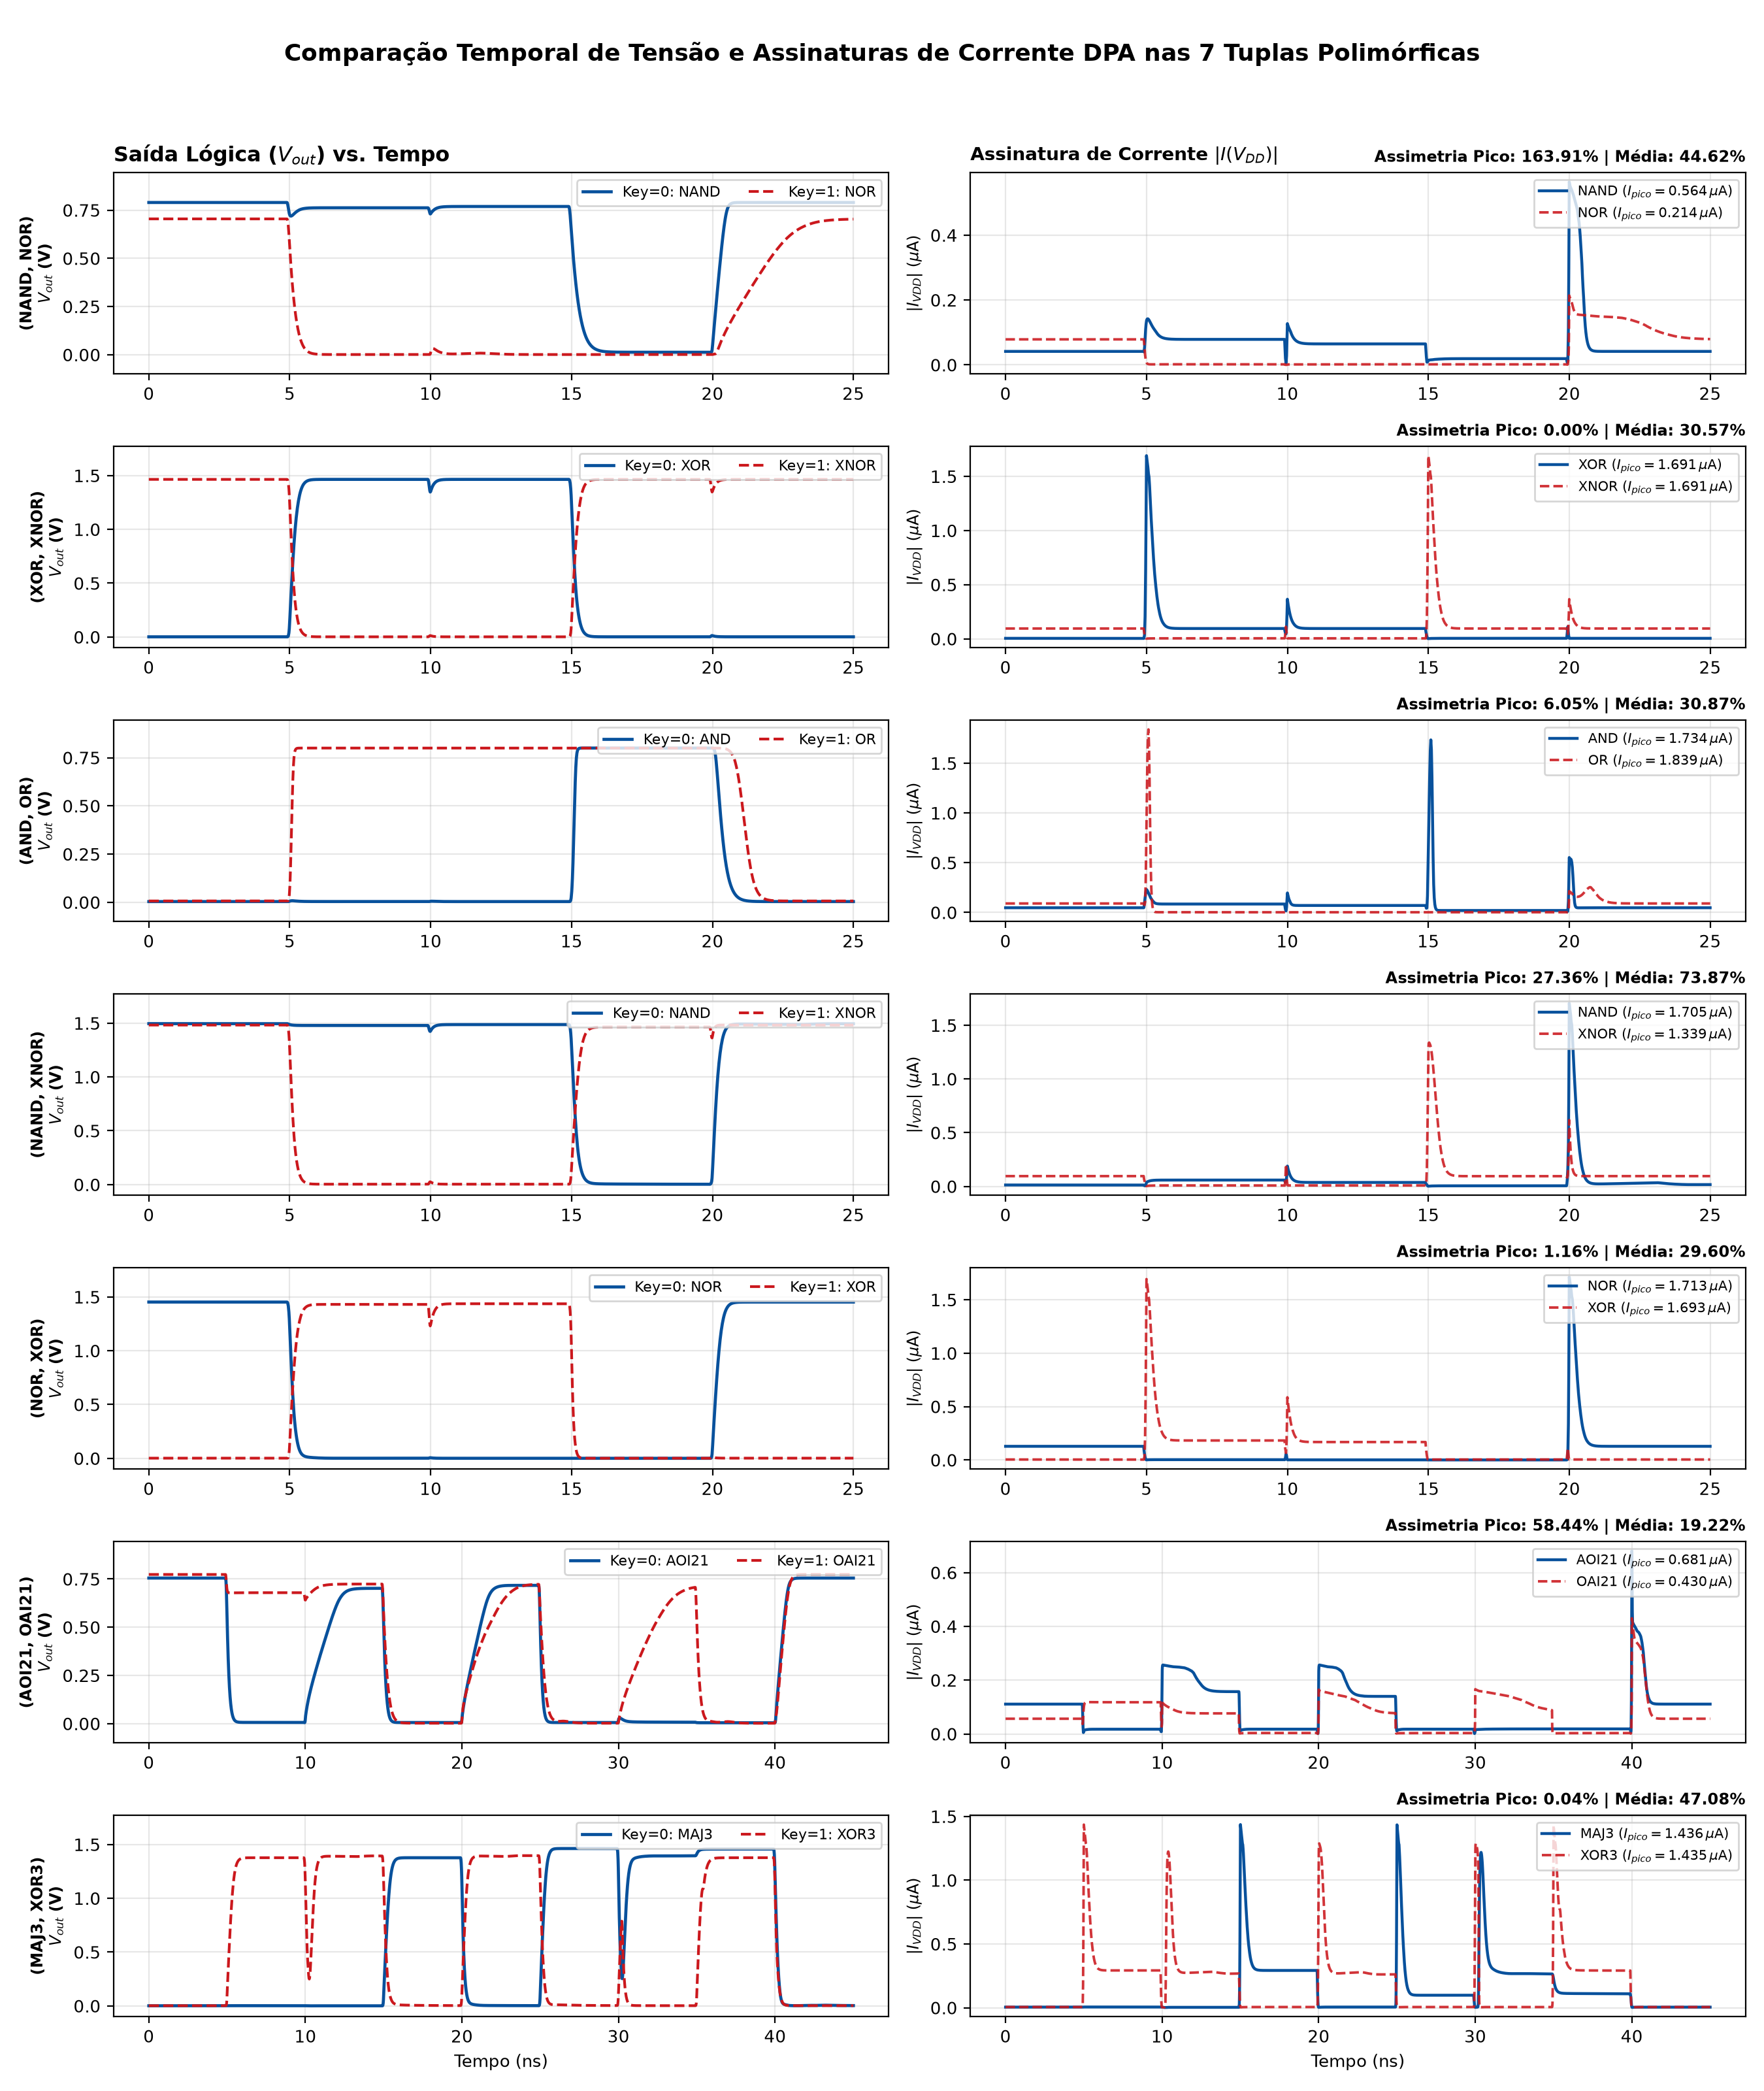
\includegraphics[width=0.90\textwidth,height=0.76\textheight,keepaspectratio]{m07_assinaturas_corrente_tuplas.png}
\caption{Assinaturas temporais de corrente $|I(V_{DD})|$ comparando $\text{Key}=0$ e $\text{Key}=1$ nas sete tuplas polim\'{o}rficas sob carga padronizada ($C_{\mathrm{load}} = 0{,}3\ \text{fF}$).}
\label{fig:m07_assinaturas}
\end{figure}

\begin{figure}[htbp]
\centering
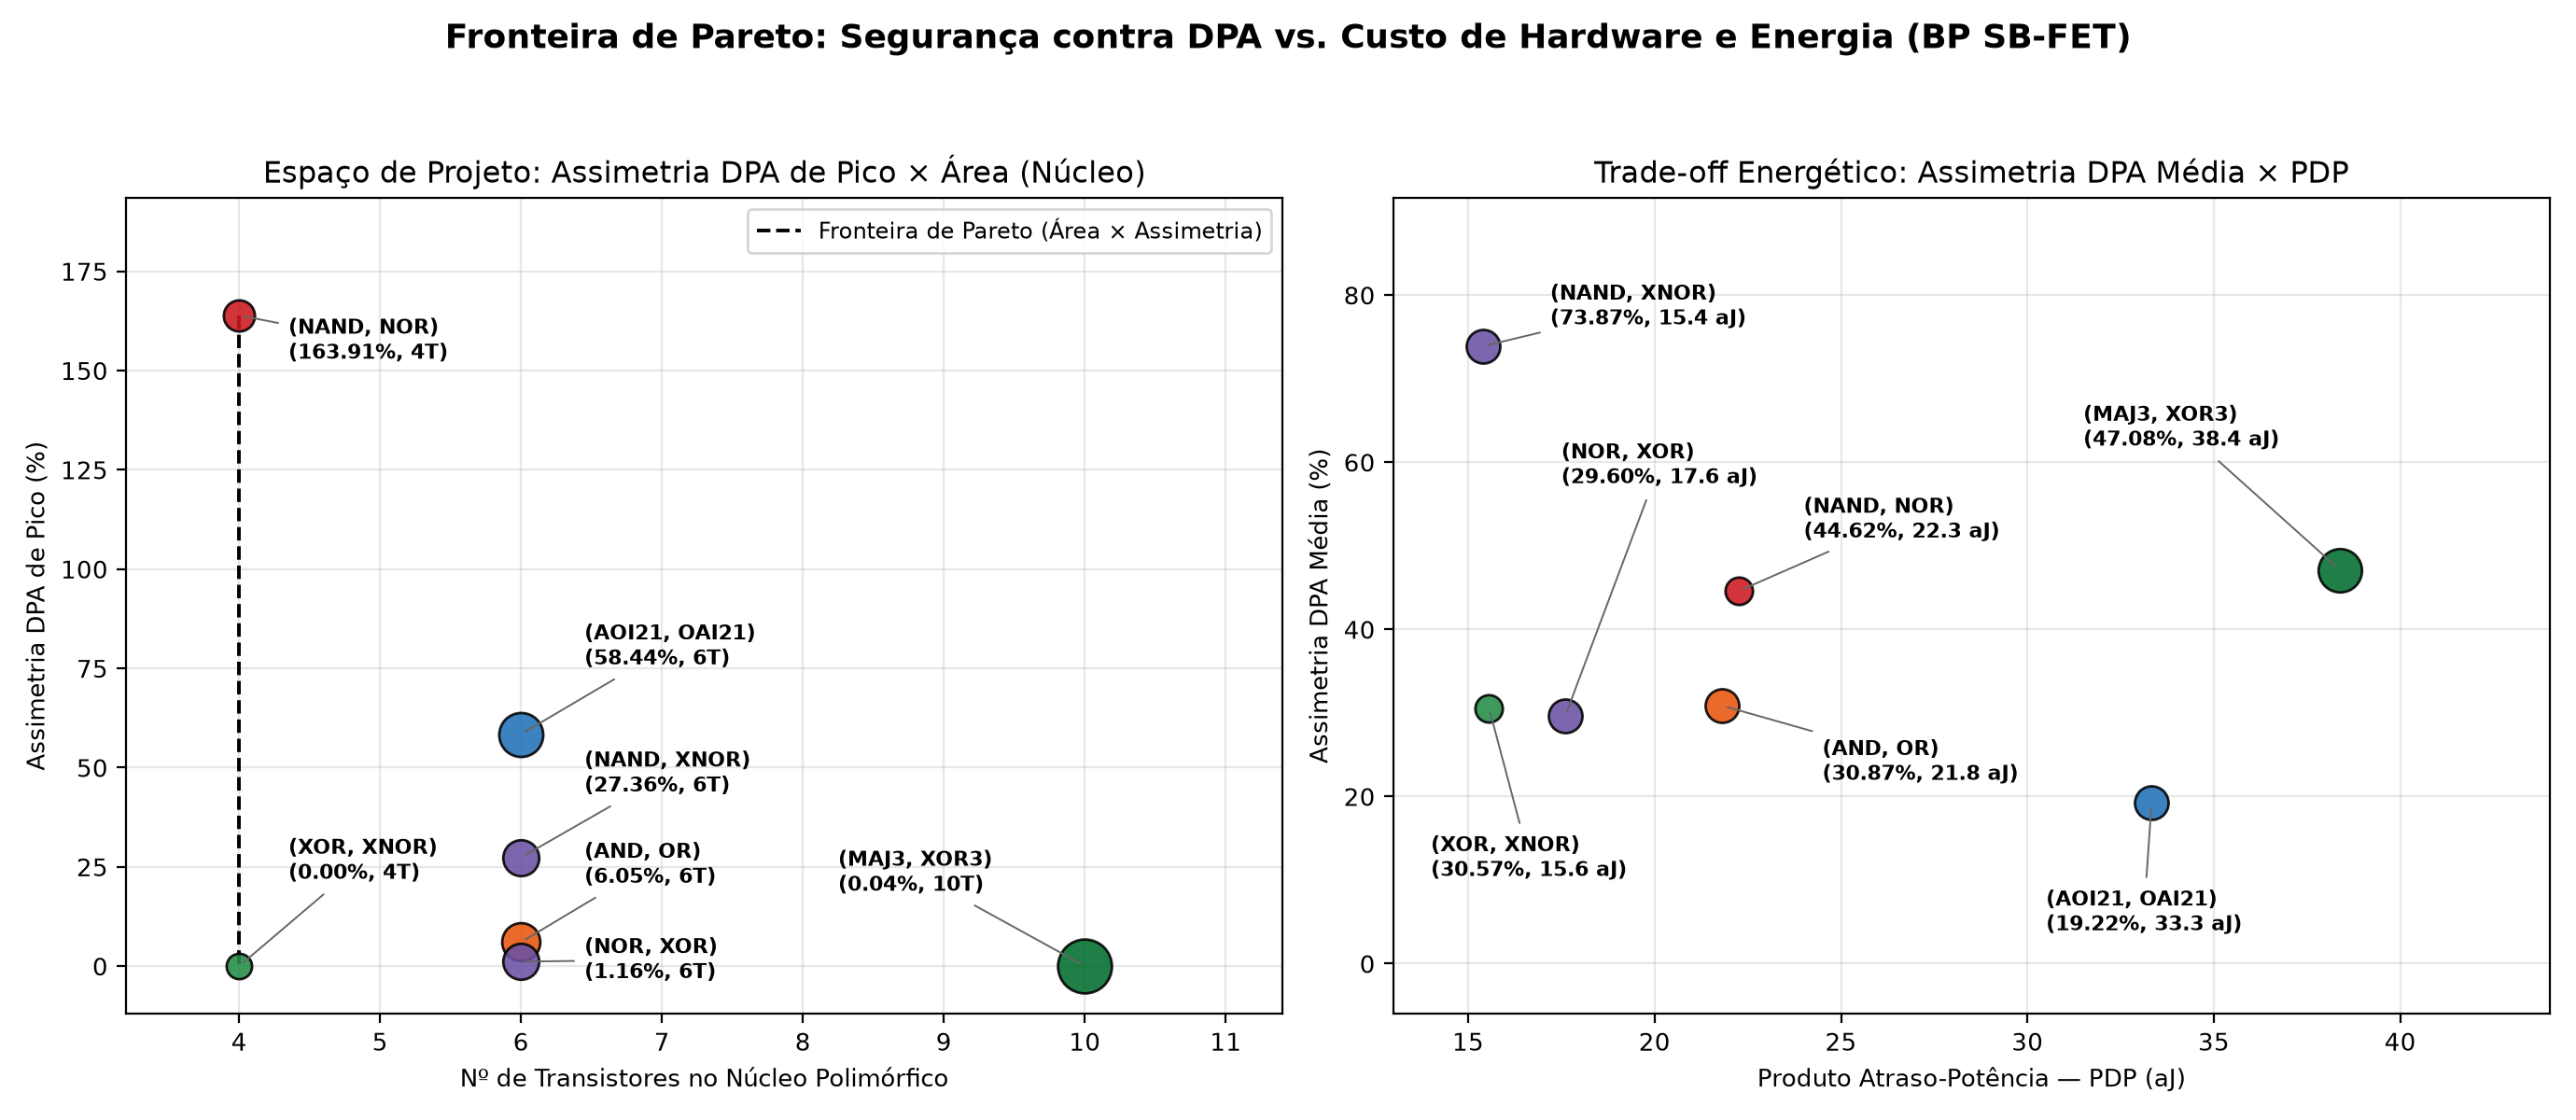
\includegraphics[width=0.92\textwidth]{m07_pareto_assimetria_vs_custo.png}
\caption{Fronteira de Pareto relacionando assimetria DPA de pico, n\'{u}mero de transistores e produto pot\^{e}ncia-atraso ($\mathrm{PDP}$) nas sete tuplas avaliadas.}
\label{fig:m07_pareto}
\end{figure}

\begin{figure}[htbp]
\centering
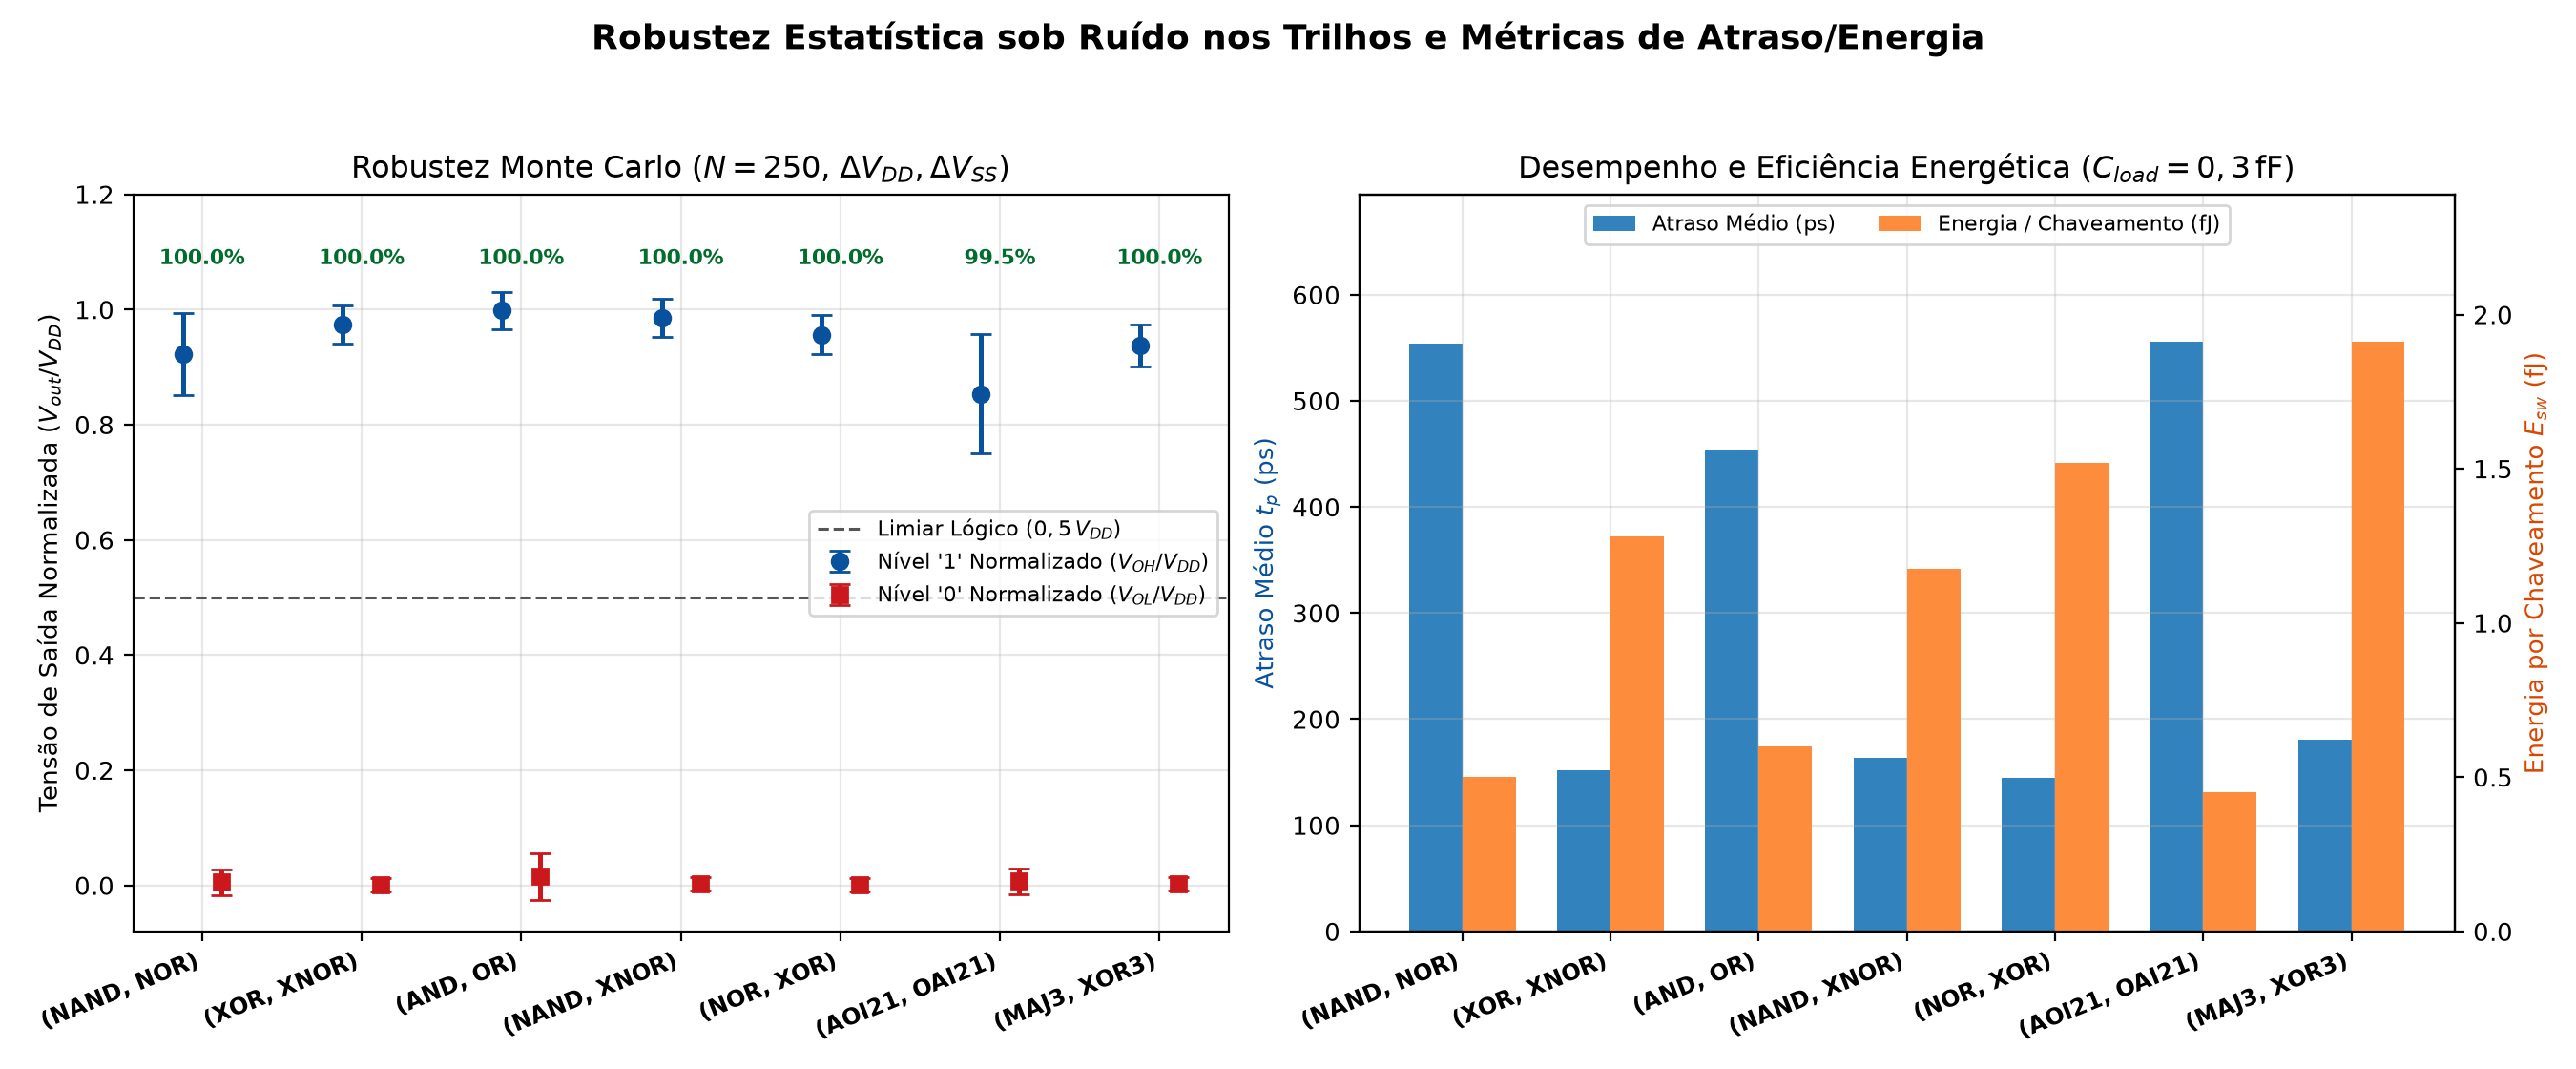
\includegraphics[width=0.92\textwidth]{m07_robustez_montecarlo_tuplas.png}
\caption{Taxa de acerto em Monte Carlo ($N=250$) sobre grade real de ru\'{i}do nos trilhos e distribui\c{c}\~{a}o de atraso e energia entre as sete tuplas.}
\label{fig:m07_mc}
\end{figure}

No \textit{benchmark} de sistema com tr\^{e}s arquiteturas de Somador Completo 1-bit (Tabela~\ref{tab:fa_perfis} e Figura~\ref{fig:m07_fa}), todos os perfis obtiveram $100{,}0\%$ de corretude funcional em $K=00$. O \textbf{Perfil 2} (baseado em tr\^{e}s portas \texttt{NAND}/\texttt{NOR} no \textit{carry}) eleva a contagem para 28T, multiplica o atraso cr\'{i}tico em $3{,}58\times$ frente ao Baseline ($177{,}72 \to 636{,}68\ \text{ps}$), aumenta o PDP cr\'{i}tico em $3{,}54\times$ ($131{,}86 \to 466{,}44\ \text{aJ}$) e exp\~{o}e uma assinatura DPA de $113{,}83\%$ no caminho de \textit{carry}. Em contrapartida, o \textbf{Perfil 3} substitui a \'{a}rvore \texttt{NAND}/\texttt{NOR} por uma \'{u}nica c\'{e}lula \texttt{(MAJ3, XOR3)} de 10T, reduzindo a contagem de n\'{u}cleo para 26T, elevando a Dist\^{a}ncia de Hamming em chave errada ($K=11$) de $68{,}75\%$ para $87{,}50\%$ e derrubando a assimetria DPA de pico no est\'{a}gio polim\'{o}rfico de $113{,}83\%$ para apenas \textbf{$0{,}04\%$}. Com atraso cr\'{i}tico de $196{,}98\ \text{ps}$ ($+10{,}8\%$ sobre o Baseline) e PDP de $155{,}19\ \text{aJ}$ ($+17{,}7\%$ sobre o Baseline e \textbf{$3{,}01\times$ inferior ao Perfil 2}), o Perfil 3 demonstra superioridade simult\^{a}nea em seguran\c{c}a, \'{a}rea e efici\^{e}ncia energ\'{e}tica.

\begin{table}[htbp]
\centering
\caption{\textit{Benchmark} arquitetural do Somador Completo 1-bit em tr\^{e}s perfis no \texttt{ngspice-47} ($C_{\mathrm{load}} = 0{,}3\ \text{fF}$).}
\label{tab:fa_perfis}
\resizebox{\textwidth}{!}{%
\begin{tabular}{l c c c c c c c c c}
\toprule
\textbf{Perfil Arquitetural} & \textbf{N\'{u}cleo} & $\sum W$ & \textbf{Corret.\ K00} & \textbf{HD (K11)} & $t_{\mathrm{cr\acute{i}t}}$ (ps) & $P_{\mathrm{m\acute{e}d}}$ (nW) & \textbf{PDP} (aJ) & \textbf{DPA Pico Carry} & \textbf{DPA M\'{e}d.\ Carry} \\
\midrule
1. Baseline (Comum, sem \textit{lock}) & 20T & $24{,}0$ & $100{,}0\%$ & $0{,}0\%$   & $177{,}72$ & $741{,}97$ & $131{,}86$ & N/A & N/A \\
2. Custo/Desempenho (\texttt{NAND}/\texttt{NOR}) & 28T & $38{,}0$ & $100{,}0\%$ & $68{,}75\%$ & $636{,}68$ & $732{,}60$ & $466{,}44$ & $113{,}83\%$ & $62{,}44\%$ \\
3. Baixa Assimetria (\texttt{MAJ3}/\texttt{XOR3}) & 26T & $38{,}0$ & $100{,}0\%$ & $87{,}50\%$ & $196{,}98$ & $787{,}87$ & $155{,}19$ & $0{,}04\%$   & $47{,}47\%$ \\
\bottomrule
\end{tabular}}
\end{table}

\begin{figure}[htbp]
\centering
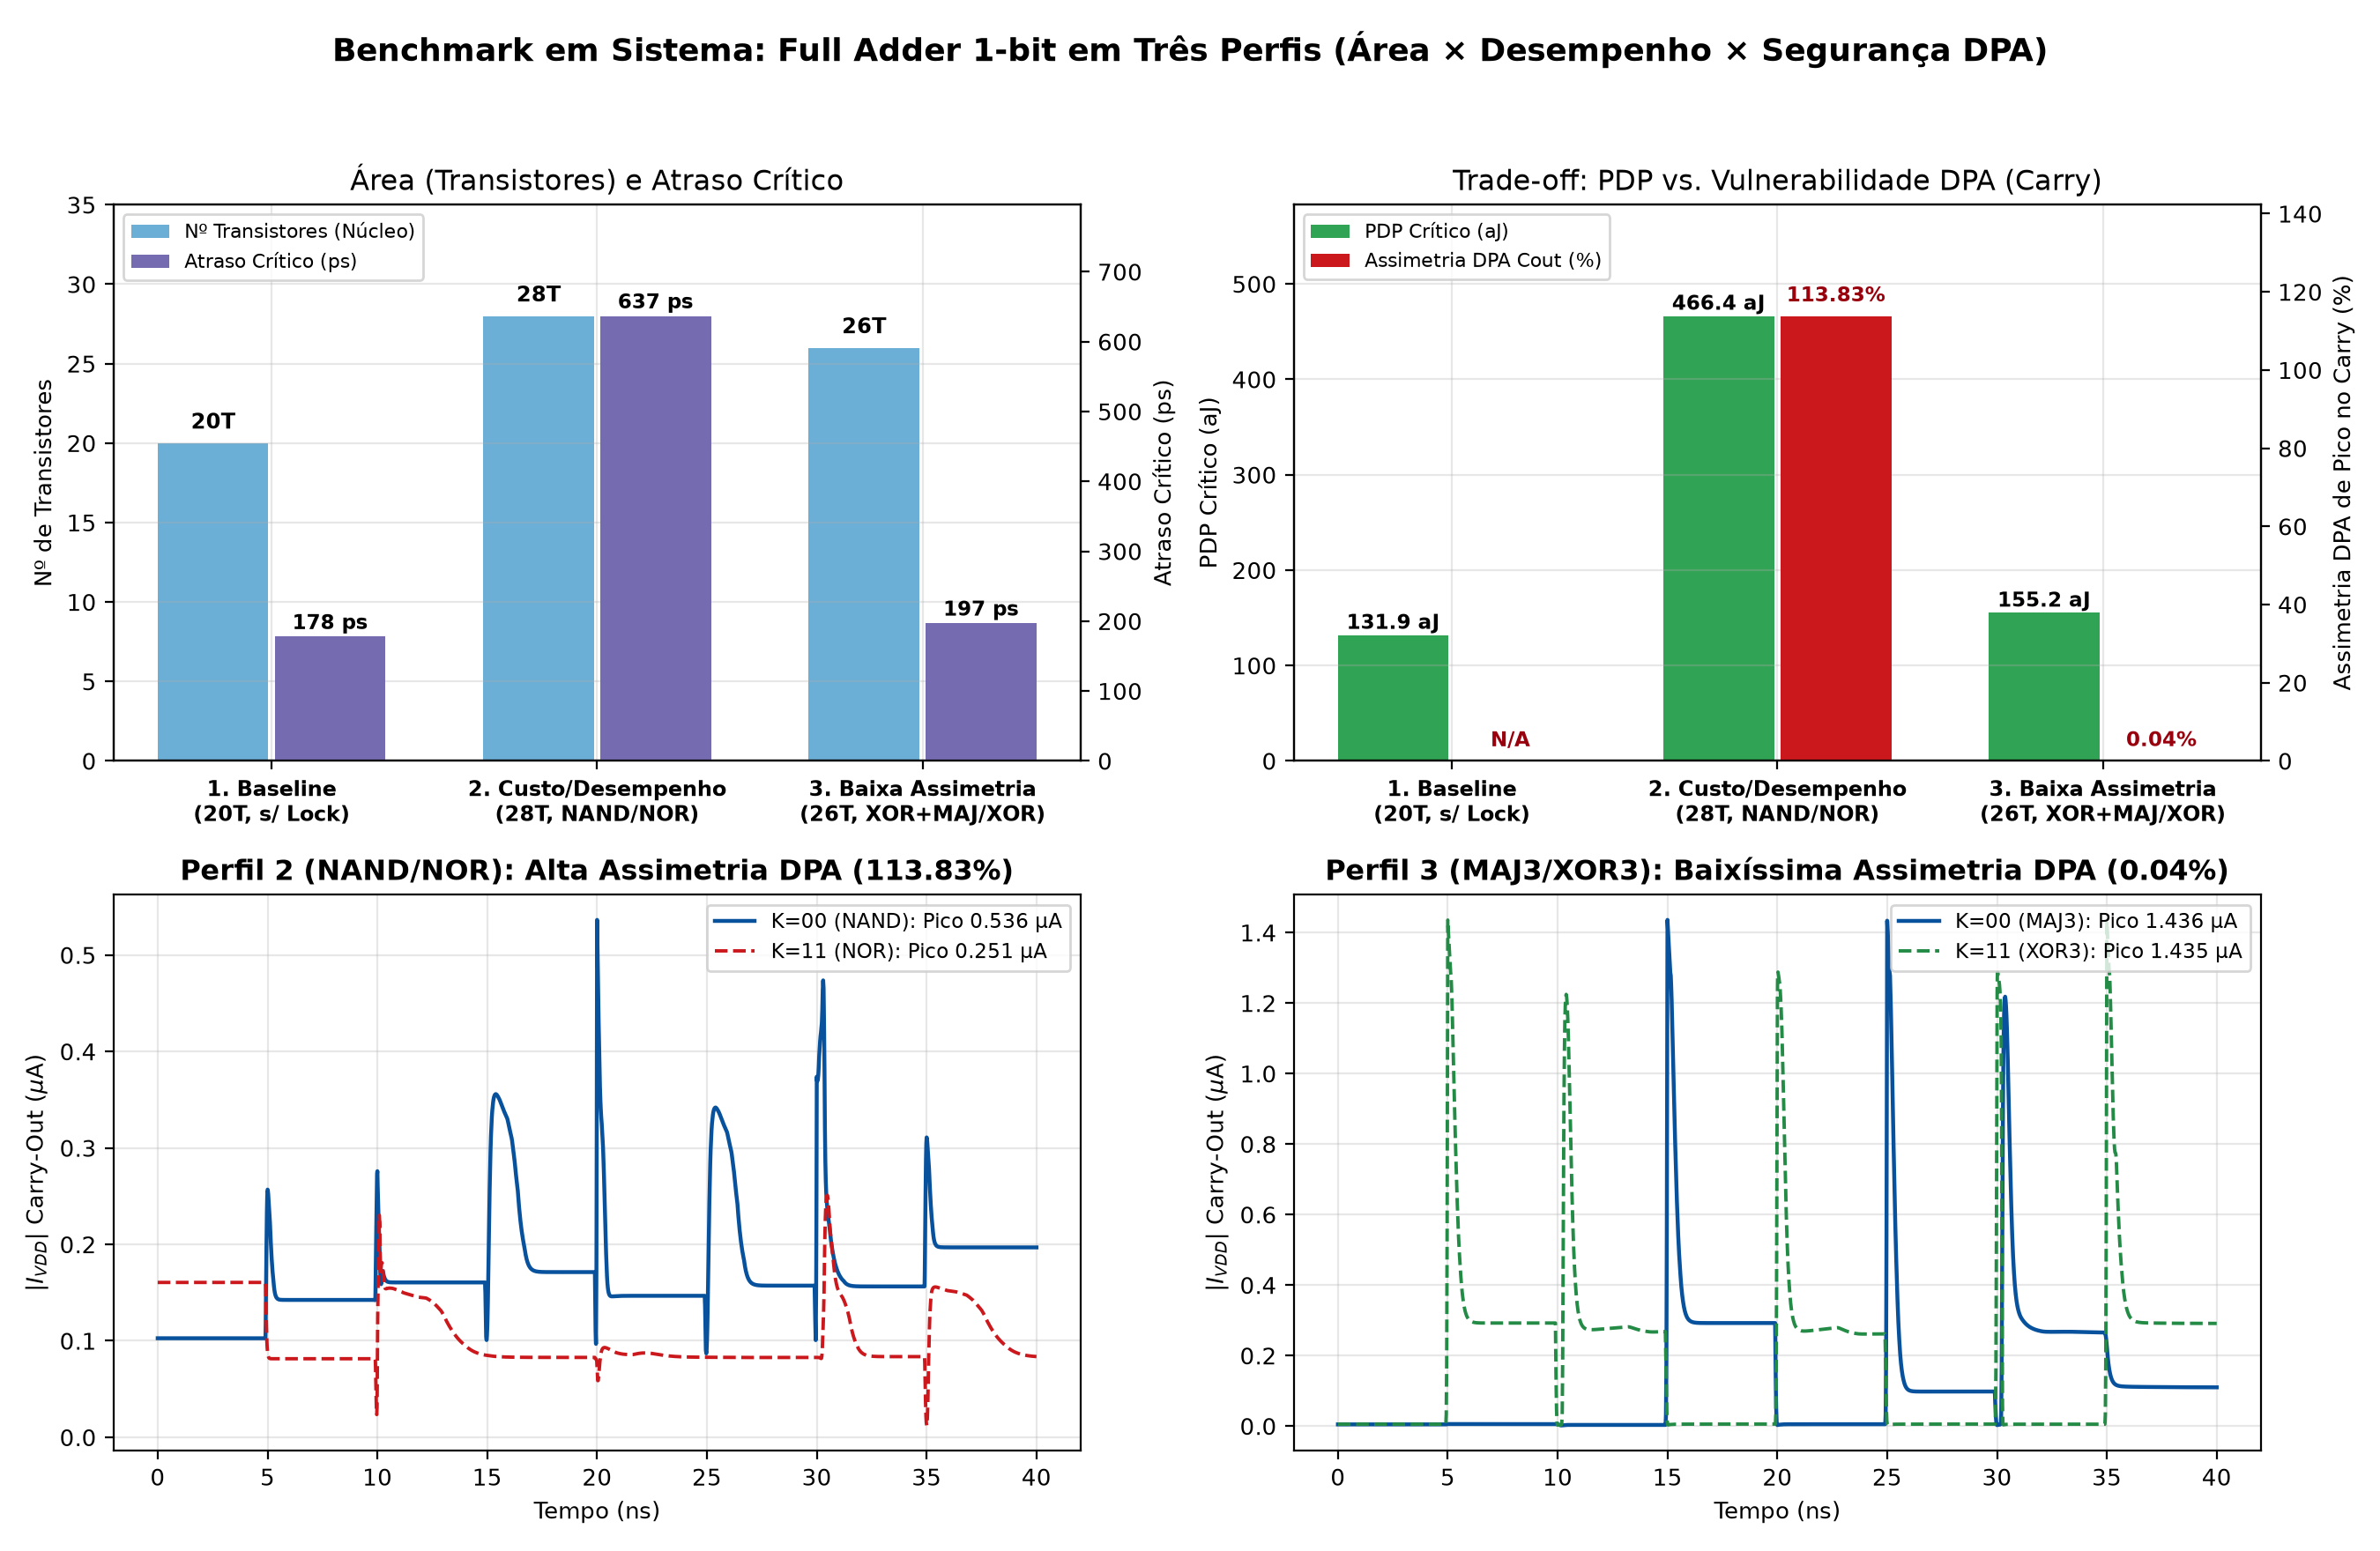
\includegraphics[width=0.92\textwidth]{m07_benchmark_full_adder_perfis.png}
\caption{Comparativo do Somador Completo 1-bit nos tr\^{e}s perfis arquiteturais quanto a contagem de transistores, atraso cr\'{i}tico, PDP, ofusca\c{c}\~{a}o (HD) e assimetria DPA no \textit{carry}.}
\label{fig:m07_fa}
\end{figure}

\subsection{Valida\c{c}\~{a}o Ponta a Ponta do Simulador Visual Interativo (\textit{BP-FET Studio})}\label{sec:res_web}

A su\'{i}te automatizada \texttt{simulador\_web/test\_simulator.py} validou integralmente a compila\c{c}\~{a}o de grafos, a simula\c{c}\~{a}o em lote no \texttt{ngspice-47} e o servidor REST da plataforma \textit{BP-FET Studio}:
\begin{enumerate}
    \item \textbf{Sete tuplas polim\'{o}rficas e inversor \texttt{INV} em alto n\'{i}vel:} todas as combina\c{c}\~{o}es de tabela-verdade e o mapeamento interno de transistores do modo \textit{Raio-X} passaram com $100\%$ de exatid\~{a}o, reproduzindo os valores de assimetria DPA de pico do M\'{o}dulo \texttt{07} (\texttt{NAND\_NOR}: $163{,}91\%$; \texttt{XOR\_XNOR}: $0{,}00\%$; \texttt{AND\_OR}: $6{,}05\%$; \texttt{NAND\_XNOR}: $27{,}36\%$; \texttt{NOR\_XOR}: $1{,}16\%$; \texttt{AOI21\_OAI21}: $58{,}44\%$; \texttt{MAJ3\_XOR3}: $0{,}04\%$; \texttt{INV}: $0{,}00\%$) em tempos de execu\c{c}\~{a}o entre $234\ \text{ms}$ (\texttt{INV}) e $7{,}04\ \text{s}$ (\texttt{MAJ3\_XOR3}).
    \item \textbf{Oito templates do cat\'{a}logo:} todos os modelos em alto e baixo n\'{i}vel foram simulados com sucesso ($0{,}65\ \text{s}$ a $14{,}31\ \text{s}$), verificando tanto os Somadores Completos dos Perfis 2 e 3 em $K=0$, quanto a invers\~{a}o f\'{i}sica de polaridade (\textit{p-FET} $\leftrightarrow$ \textit{n-FET}) na c\'{e}lula \texttt{NAND}/\texttt{NOR} 4T e a reten\c{c}\~{a}o ($\Delta V > 0{,}7\ \text{V}$ em $12\ \text{ns}$, \texttt{XPU1} como \textit{p-FET}) seguida de colapso ($\Delta V < 0{,}25\ \text{V}$ em $28\ \text{ns}$, \texttt{XPU1} como \textit{n-FET}) na SRAM 6T.
    \item \textbf{Cascata mista multidom\'{i}nio e API HTTP:} um circuito arbitr\'{a}rio encadeando $0{,}8\ \text{V} \to 1{,}5\ \text{V} \to 0{,}8\ \text{V}$ (\texttt{NAND\_\allowbreak NOR} $\to$ \texttt{XOR\_\allowbreak XNOR} $\to$ \texttt{AND\_\allowbreak OR}) com condicionamento autom\'{a}tico de n\'{i}vel foi compilado e validado em $5{,}87\ \text{s}$ ($100\%$ exato em $\text{Key}=0$ e $\text{Key}=1$), e todas as rotas HTTP/JSON (\texttt{/}, \texttt{/api/\allowbreak tuples}, \texttt{/api/\allowbreak templates}, \texttt{/api/\allowbreak simulate}) responderam com c\'{o}digo $200$.
\end{enumerate}
